% -*- Mode:TeX -*-

%% The documentstyle options along with the pagestyle can be used to generate
%% a technical report, a draft copy, or a regular thesis.  You may need to
%% re-specify the pagestyle after you \include  cover.tex.  For more
%% information, see the first few lines of mitthesis.sty. 


\documentclass[12pt]{report}

\usepackage{fullpage}
\usepackage{epsfig}
%\usepackage{fancyhdr}
% \usepackage{changebar}

\setcounter{tocdepth}{1}  % Display contents down to section
\pagestyle{plain}

%% This bit allows you to either specify only the files which you wish to
%% process, or `all' to process all files which you \include.
%% Krishna Sethuraman (1990).

\typein [\files]{Enter file names to process, (chap1,chap2 ...), or `all' to
process all files:}
\def\all{all}
\ifx\files\all \typeout{Including all files.} \else \typeout{Including only \files.} \includeonly{\files} \fi


% Change ``Bibliography'' to ``References''
\makeatletter
\def\thebibliography#1{\chapter*{References\@mkboth
 {REFERENCES}{REFERENCES}}\list
 {[\arabic{enumi}]}{\settowidth\labelwidth{[#1]}\leftmargin\labelwidth
   \advance\leftmargin\labelsep
   \usecounter{enumi}}
   \def\newblock{\hskip .11em plus .33em minus .07em}
   \sloppy\clubpenalty4000\widowpenalty4000
   \sfcode`\.=1000\relax}
\makeatother

\begin{document}

\newcommand{\kod}[0]{{\tt kod }}
\newcommand{\bof}[0]{{\tt bof }}
\newcommand{\rsc}[0]{{\tt rsc }}
\newcommand{\makebgf}[0]{{\tt makebgf }}
\newcommand{\bgf}[0]{{\tt .bgf }}

% Commands for formatting file-format grammar
\newenvironment{protocol}
	{\begin{tabbing}
	 100 \= bytes Bytes in field \= \kill}
	{\end{tabbing}}

\newcommand{\nonterminal}[1]{{\it $<${\bf #1}$>$}}
\newcommand{\newnonterminal}[1]{\nonterminal{#1} = \\}
\newcommand{\pline}[2]{#1 \> \> #2 \\}   % ``Protocol line''
\newcommand{\plineindent}[2]{\> #1 \> #2 \\}

% -*-latex-*-

\title{Meridian 59 Documentation}
\author{Andrew Kirmse \and Christopher Kirmse}
\date{September 30, 1997}

\begin{titlepage}
\maketitle
\end{titlepage}

\pagestyle{plain}
%\pagestyle{fancy}

%\fancyhead[C]{Meridian 59 Documentation by Andrew and Christopher Kirmse}
%\setlength{\headrulewidth}{0in}
%\tableofcontents
\include{contents}
% Chapter 1--Introduction
\chapter{System overview and philosophy}

The BlakSton game system is a set of programs used to develop and run
a large-scale persistent world.  The system consists of a server, a
client, and a group of tools.  All of the programs run under Win32.
At present, the only instance of the system is the roleplaying game
Meridian 59.

The server runs at a central location and accepts TCP/IP connections
from remote clients.  It also runs an interpreter for an embedded
language called Blakod, which has been specifically designed for
implementing persistent world games.  A built-in administration mode
allows the server to be remotely configured while it is running.

Players run the client on their local machines and use their username
and password to access the server.  The client displays a graphical
view of the player's vicinity, and allows the player to move, speak,
and interact with other objects in the world.  The client/server
protocol has been designed so that it will use less than 9600 bits per
second, a reasonable lower limit for modem users.

The tools consist of a Blakod byte compiler, a room editor, a bitmap
compiler, a hotspot editor, and third-party libraries for performing
compression and encryption, ftp file transfer, and sound mixing.

The system was designed to support many different games using the same
client and server.  On the server side, all of the game play resides
in Blakod, so that the server itself is independent of the details of
any one particular game.  On the client side, most of the
game-specific interface and data components reside in DLLs outside the
main client executable.  The client/server protocol is also fairly
general, and it can be easily extended.

BlakSton is also meant to be a completely dynamic system.  The server
can reload Blakod at any time, so that game play can be modified
without shutting down the server.  In addition, many of the server's
configuration options can be changed while the server is running.  The
server's protocol tables reside in a separate module that can be
reloaded at any time.  Any piece of the client can be modified by
requiring users to download changes.  Additional downloadable files
can be added while users are still connected.

Security is a serious problem in an online environment.  Through a
combination of encryption and careful protocol design, the system can
prevent the most obvious attacks, and can detect most others.  Almost
all data from the client is verified, so that a malicious entity
should not be able to obtain an advantage in game play, or deny
service to others.

Another design goal was reliability, even at the expense of some
performance.  The server has not experienced a software fault in over
25,000 hours of commercial operation, and there are no known ways to
crash the client.  Although the Blakod for Meridian 59 contains
numerous errors, the server simply reports the errors and continues
normal operation.  It was the overriding design goal of reliability
that allowed the system to become a commercial success.

Meridian 59 is a medieval roleplaying game that uses the BlakSton
system.  Players try to improve their characters through a combination
of combat, magic spells, and teamwork with other players.  An alpha
version of the game appeared on December 15, 1995, and a commercial
version launched on September 27, 1996.


% Chapter 1--Introduction

\chapter{Architecture}
%%%%%%%%%%%%%%%%%%%%%%%%%%%%%%%%%%%%%%%%%%%%%%%%%%%%%%%%%%%%%%%%%%%%%%%%%
\section{The server}

The BlakSton server is designed to be a generic large-n world game
server which could potentially be used for several different online
games.  Keeping most game-specific code out of the server has made it
possible to make a robust server which has not crashed since the
system has been commercially available (as of this writing).

In order to make the server incredibly safe, I would estimate that
over half of the code is for error checking.  For example, even though
all Blakod objects' references to other objects are always valid, the
return value of \texttt{GetObjectByID} is checked against NULL.
Instead of using the now-common practice of using assertions to abort
a program when unforeseen circumstances arise, the server treats these
as possible error conditions and logs the problem, instead of
aborting.  Since even a single crash could cost hundreds or thousands
of dollars of customer service time, this was deemed crucial to the
game's success.

Since there is only a minimal amount of game-specific code in the
server, the overall design of the server is quite clean (and fairly
obvious).  The heart of the server is the Blakod interpreter, which
runs the actual game code.  Blakod calls are made when messages are
received from clients or timers expire.  Since the Blakod interpreter
is single threaded, only one call into Blakod exists at any time.
This puts several demands upon the interpreter.  First, it must be
rather fast, so that the server does not become backed up by client
requests.  Second, it must endeavor to prevent infinite loops or
infinite recursion in Blakod so that one poorly written Blakod
function does not hang the entire system.

To support the Blakod interpreter, the server has modules that handle
the storage of Blakod objects, Blakod list nodes, Blakod strings,
Blakod resources, Blakod strings, Blakod timers, and callback
functions.  These callback functions, called C code functions, exist
so that Blakod may interact with the server, since Blakod has no
inherent input or output.

The server's primary task outside of Blakod interpreting is keeping
track of network connections made by clients.  It needs to verify user
logins, allow administration of the game, and parse client messages
from the network to send the necessary messages to Blakod.

Client logins are mapped to accounts stored on the server.  Each different
physical person has his/her own account on the server, which they access
by logging in with their own account name and password.  Internally, the
server stores a unique account number for each account.  Each time an account
is created, it is given a new account number one greater than the previous
largest account number.  When an account is deleted, the account number
is no longer in use, and unless it was previously the largest account number,
is not reused.  Since account numbers are 32 bit integers, there is little
chance of them ever rolling over.

The server also keeps a map between account numbers and user objects in
the game.  Each account may have more than one user object mapped to it.
When a client requests that it would like to enter the game, the server
sends it a list of user objects which it may choose from.  This gives
the user the option of using any of their available characters in the game
each time he/she logs in.

The server maintains and controls all of the state associated with
avatar objects.  This information is all stored in the Blakod
properties of the object.  The client knows the avatar's position,
associated bitmap files, and a set of properties called ``object
flags''.  These flags are used to indicate that the client should
display the avatar with special effects, such as invisibility, color
translations, or shadowform.  The client also knows if the player is
paralyzed or resting, so that it can prevent user motion and running,
respectively, without a network round trip to the server.  The client
updates the server's knowledge of a player's position at most once a
second, to reduce server CPU usage.

\subsection{Network interface and threads}

The BlakSton Server communicates with other computers using TCP/IP
through the WinSock 1.1 interface.  WinSock 2 implementations are only
now available, and it is not known what benefits the server could
derive from using the new WinSock standard.

The server has two threads of execution.  The primary thread performs
nearly all tasks, including interpreting blakod and parsing messages
from clients.  The second thread is the interface thread.  It runs the
window interface and also performs asynchronous input/output on the
sockets that the server uses to communicate to clients.  The
programming overhead of using semaphores to lock access to the
server's buffers for client communication is onerous and difficult to
maintain.  However, it has proven successful.  Each time that any
thread needs to access either the input or output thread for a socket,
it first gets access to the buffer's semaphore, waiting for it
to be available if the other thread holds it.  The code then
reads or writes data from or to the buffer, and then releases the semaphore.
This is a standard way for multiple threads in a process to share
memory.

The interface thread is quite simple.  There is a main loop that
dispatches all Window events to the appropriate handler functions.
There are several GUI events that are used to provide simple ways to
save the game, terminate the server, and bring up an outdated help
system.  Also, the administrator commands sent by the GUI are passed
to the main thread to be handled there.

The only other events that the interface thread receives are events
pertaining to sockets.  The three different messages are sent when
bytes are received, the internal WinSock outgoing buffer changes from
a full to a non-full state, or the socket is closed.

When the interface thread receives bytes on a socket, it reads those
bytes and adds them to a queue for the appropriate session.  A session
is a data structure maintained by the server for each connected
client.  It includes input and output data queues, the session state
(whether the client is just logging in, is at the main menu, or in the
game), as well as the client's IP address, CPU type, and screen size.

After the bytes are added to the appropriate session's queue, the main
thread is signalled.  The main thread, when it receives a time
quantum, examines each session's queue and proceeds to parse new bytes
in each queue.

When the interface thread is notified that a socket's WinSock outgoing
queue is no longer full, it looks in the server's outgoing queue for
that session.  If there are bytes waiting to be sent, then the
interface thread immediately sends the queued bytes over the socket
and resets the queue.

When the interface thread is notified that a socket has been closed,
then the main thread is sent a message to close the appropriate
session and free any memory allocated for the session.

\subsection{Event handling}

The previous section describes the window events handled by the interface
thread.  Here is a description of the events sent to the main thread:

\begin{description}
\item[WM\_BLAK\_MAIN\_READ] The interface thread sends this when it reads
bytes from a client; the main thread responds to this message by parsing
the message if it is complete and sending the data to Blakod if necessary.

\item[WM\_BLAK\_MAIN\_RECALIBRATE] Sent by the main thread when the timer
node in the front of the timer node list changes, so we can reset the
time we'll wait for an event.  This is only an issue if a new timer is 
created that is set to go off before any other timer in the system.

\item[WM\_BLAK\_MAIN\_DELETE\_ACCOUNT] Sent by the main thread when an
administrator deletes an account.  We handle this by deleting the account.

\item[WM\_BLAK\_MAIN\_VERIFIED\_LOGIN] Sent by the main thread when
the billing system signals a valid login.  The appropriate session is then logged in.

\item[WM\_BLAK\_MAIN\_ALLOW\_LOGINS] Send by the main thread when
the billing system is enabled and has finished its initialization.  We respond
by calling \texttt{accept} on a socket to begin to allow client logins.

\end{description}

\subsection{Communication buffers}

Although WinSock has internal input and output buffers for each socket, I
chose to implement an additional level of buffering in BlakServ itself.  This allows
the server to theoretically read and write any length messages, no matter their
length, because the server buffers are implemented as a list of buffers.  This
has not been exploited, but is available.

The buffering system in the server is quite simple.  A session buffer list is
a singly linked list of \texttt{buffer\_node} structures, which contains a pointer
to a block to send (up to 5000 bytes in length), the actual length of the block,
and a pointer to the next node in the list.

To send bytes to a client session, the server calls a function called
\texttt{SendBytes} with the session structure, buffer, and buffer size to
send to the session.  \texttt{SendBytes} checks to see if the session already has
a send buffer list.  If the session is backed up, then the new block of bytes is
added to the end of the buffer list, and if necessary allocating new buffers on 
the end of the list.  If the session is not backed up, then the bytes are sent
straight to WinSock to send to the client.  If this call fails, then the bytes
are put in a buffer list and stored in the session structure.

Unlike transmitted data, all received data is always placed in a buffer list when
it is received by the interface thread.  The interface thread then sends a message
to the main thread that tells it to process the bytes in the appropriate session.


\subsection{Blakod interpreter}

When a complete message arrives from a client or a timer goes off, the
server sends a message to a Blakod object.  Client messages are always
sent to the Blakod object associated with the client's account, which
is always of the class \texttt{user} or descends from this class.  
Client messages can have up to 15
parameters.  Timer messages can be sent from the server to any object,
and have no parameters.

Parameters are actually referenced as local variables by the compiled
Blakod (called \emph{bkod}).  If a message gets passed $n$ parameters
and uses $m$ local variables, then then local variables $0..n-1$ are
actually parameters, and local variables $n..n+m$ are used as local
variables.

The core of the Blakod interpreter iterates through the bkod
instructions of one message handler.  Instructions can only modify
local variables for the message handler or properties of the object.
The only instructions that can communicate outside of the current
objects are CALL instructions, which invoke C code in the server.  A
complete list of the C functions is in the next section.

Some of the C code functions are quite simple, such as \texttt{Bound}
which is a combined min and max function.  However, most of the C code
functions are rather complex and do things that could not otherwise be
done in Blakod.  The most important may be \texttt{Send}.  This
function takes an object, a message name, and a set of parameter names
and values and invokes the Blakod interpreter on the destination
object with the given message and parameter values.  Since this is
implemented as a simple recursive call in the server, the original
call is suspended while the sub-call takes place.  Also, since the
server stack is used for this recursion, there is a check to make sure
that the recursion does not go on forever (such as in a Blakod
function that was infinitely recursive).  If the call stack gets too
deep, it is aborted and an error is printed in the error log.  If this
check did not exist, the server would crash.

The other two critical C code functions are \texttt{AddPacket} and
\texttt{SendPacket}.  These functions allow Blakod to build up a
packet of data and then send it over the network to a client.
\texttt{AddPacket} takes an even number of parameters; the odd number
parameters must be integers which specify the number of bytes of the
following parameter.  For example, since many player statistics are
known to be small, the protocol only allocates one byte for each
statistic.  So although object properties and local variables are
always four bytes, only the low one or two bytes are sometimes sent,
when the protocol calls for it.  \texttt{AddPacket} takes the values
and adds them to a global output buffer.  Once a full packet is built
up (from one or more \texttt{AddPacket} calls), the Blakod then calls
\texttt{SendPacket} along with a session number so the server knows
which client to send the packet to.  The user object is sent this
session number each time a client logs in, and stores it for use in
calls to \texttt{SendPacket}.

\texttt{SendPacket} adds a header to the data packet, and checks the
output queue for the destination session.  If it is empty, the server
calls the WinSock send function to instantly send the data to the
client.  If this fails, it adds the packet to the server's output
queue for the session which the interface thread will send later, when
it gets a message from WinSock that the send buffer is no longer
empty.  If the server's output queue is already non-empty, the packet
is just added to the queue.

\subsubsection{Built in functions}

\begin{description}

\item[create] Takes a class.  Creates a new object of the specified class, and sends it 
the \texttt{Constructor} message.
\item[isclass] Takes two parameters, an object and a class.  Returns the 
integer 1 if the object is of the specified class or any of the class' descendants.

\item[getclass] Takes an object.  Returns the class of the specified object.

\item[send] Takes an object, a message, and any number of parameters.  
Immediately sends the given message to the given object, with all of the specified parameters.
\item[post] Takes an object, a message, and any number of parameters.
Queues up the message in the Blakod message queue.  See the next section.

\item[debug] Takes any number of parameters.
Prints all parameters to the debug log, which is on the BlakServ
interface and \texttt{debug.txt}.

\item[addpacket] Takes any number of pairs of parameters.  The odd numbered
parameters are the lengths to send of the even numbered parameters.  Adds
the specified data to a send buffer, which can be sent to a particular client
with \texttt{SendPacket}.

\item[sendpacket] Sends any buffered up bytes (added by \texttt{addpacket}) to
the given session.  The buffer is then cleared.

\item[sendcopypacket] Sends any buffered bytes to the given session, while leaving
the buffered up bytes in place to be sent again.
 
\item[clearpacket] Clears the buffer of bytes to send to a session (in essense,
it cancels any \texttt{addpacket} calls since the last \texttt{sendpacket}).

\item[getinactivetime] Takes a session id.  Returns an integer of the number
of seconds since the server has received bytes from the session's client.
   
\item[stringequal] Takes two parameters, both of which can be either strings
or resources.  Returns the integer 1 if the two parameters are different only
in capitalization and spacing; otherwise returns the integer 0.

\item[stringcontain] Takes two parameters, both of which can be either
strings or resources.  Returns the integer 1 if any substring of the first parameter 
differs only in capitalization and spacing from the second parameter; otherwise
returns the integer 0.

\item[setresource] Takes a dynamic resource (a player's name) and a resource.  Sets
the dynamic resource to the string value of the resource.

\item[parsestring] Takes a string, a debug string (string contained in quotes
in Blakod source code), and a message.  Calls the C runtime function \texttt{strtok}
on the string using the debug string as separators, and calls back the calling
object with the specified message for each parsed string.  Only used for parsing
the destination field of mail messages.

\item[setstring] Takes a string and a resource.  Sets the string to the string
value of the resource.

\item[createstring] Returns a new, zero length string.

\item[createtimer] Takes an object, a message, and an integer number of milliseconds.
Adds a node to the timer queue to call the specified message on the specified object
in the specified amount of time.  Returns the timer id, which can be used in calls
to \texttt{deletetimer} and \texttt{gettimeremaining}.

\item[deletetimer] Takes a timer id.  Removes the timer from the timer queue.

\item[gettimeremaining] Takes a timer id.  Returns the integer number of milliseconds
before the specified timer is set to go off.

\item[createroomdata] Takes a resource, which must specify the filename of a room
file.  Loads the server movement grid in the specified room file and returns a
room id, which as an integer that is different from the room id of any other loaded room.

\item[roomdata] Takes a room id.  Returns a list of length 3 containing the 
grid row size of the room, the grid column size of the room, and the security
number of the room.

\item[canmoveinroom] Takes a room id, a source row and column, and a destination
row and column.  The destination row and column must specify a square that directly
neighbors the source square.  Using the server movement grid of the specified room,
returns 1 if an object is able to move from the source row and column to the destination
row and column; otherwise returns 0.

\item[cons] Takes two parameters; the first can be any value, the second must be a 
list.  Adds the first element to the beginning of the list, by creating a new list
node.

\item[first] Takes a list.  Returns the first element of the list.

\item[rest] Takes a list.  Returns the list without its first element.

\item[length] Takes a list.  Returns the length of the list.  A nil list has
length zero.

\item[nth] Takes a list and an integer (call it $n$).  Returns the $n$th element
of the list.

\item[list] Takes two parameters.  Returns a two element list, whose first element
is the first parameter and second element is the second parameter.

\item[islist] Takes one parameter.  Returns 1 if the parameter is a list; otherwise
returns 0.

\item[setfirst] Takes a list and any value.  Sets the first element of the list
to be the specified value.

\item[setnth] Takes a list, an integer (call it $n$), and any value.  Sets the
$n$th element of the list to be the specified value.

\item[dellistelem] Takes a list and any value.  Returns the list with the first
occurrence of the specified value removed from the list.

\item[gettime] Returns the number of seconds since January 1st, 1996.

\item[abs] Takes one integer.  Returns the absolute value of the integer.

\item[bound] Takes an integer (call it $n$) and two values which can be integers or nil.  
Call the first of these $a$ and the second $b$.  If $a$ and $b$ are both nil, then this
function returns $n$.  If $a$ is nil and $b$ is an integer, then it returns min($n$,$b$).
If $a$ is an integer and $b$ is nil, then it returns max($n$,$a$).  If both $a$ and $b$
are integers, returns min(max($n$,$a$),$b$).

\item[createtable] Creates a new hash table with 2999 available entries.  Returns a table
id which uniquely identifies the newly created hash table.

\item[addtableentry] Takes a table id, a key value, and a data value.  Using the
hash function from the ELF file format, calculates the hash value of the key and
inserts the key value and data value into the table using open hashing.

\item[gettableentry] Takes a table id and a key value.  Returns the data value
associated with the key value from the specified table.

\item[deletetableentry] Takes a table id and a key value.  Deletes the data value
associated with the key value from the specified table.

\item[deletetable] Takes a table id.  Deletes the entire table.
   
\item[random] Takes two integers.  Returns an integer randomly chosen from the closed
interval defined by the two integers.

\end{description}

\subsubsection{Objects}

The most important data in BlakServ are Blakod objects.  They are stored in one large,
dynamically sized array of the following structure:
\begin{verbatim}
typedef struct
{
   int object_id;
   int class_id;
   Bool deleted;
   int garbage_ref;
   int num_props;
   prop_type *p;
} object_node;
\end{verbatim}

Here is what each element of the object node structure means:

\begin{description}
\item[object\_id] This value is the same as the object's index in the object array.
\item[class\_id] This specifies the class of the object.
\item[deleted] This is used by the garbage collector to keep track of which
objects are not referenced and need to be deleted.
\item[garbage\_ref] This is used by the garbage collector to store what this object's
new object id will be after the garbage collection is done.
\item[num\_props] This is the number of properties used by this object.
\item[p] This is the actual array of property values for this object.
\end{description}

Initially the array is allocated to store ten thousand objects.  However, as the game
runs, objects are created, using up this space.  Over time, ten thousand objects
may not be able to hold every object.  In this case, the array is reallocated
at twice its previous size.  This means that the array is never ``full'', because
even if there are no open entries, it will automatically be resized to store more
objects.

\subsubsection{List nodes}

Another key part of Blakod is list nodes.  Although they act much like
LISP lists, all operations are destructive--the server itself never
makes a copy of changed list.  This reduces memory usage considerably,
but requires more care on the Blakod programmer's part.  They are stored
in one large, dynamically sized array of the following structure:
\begin{verbatim}
typedef struct
{
   val_type first;
   val_type rest;
   int garbage_ref;
} list_node;
\end{verbatim}

Here is what each element of the list node structure means:

\begin{description}
\item[first] This is a Blakod value (4 bits tag, 28 bits data) of the
current node in the list.
\item[rest] This is a Blakod value of the next node in the list (or nil
if it is the end of list).  If this is not nil or a list node, then
it works exactly like dotted pairs in LISP.
\item[garbage\_ref] This is used by the garbage collector to store what this
list node's new list node id will be after the garbage collection is done.
\end{description}

\subsubsection{Resources}

Resources are a simple construct used to prevent the server from having to
send the actual text of preprogrammed strings over the network every time
they are used.  They are defined in the resource section of a Blakod source
file, and stored in the server in a linked list of the following structure:
\begin{verbatim}
typedef struct resource_struct
{
   int resource_id;
   char *resource_val;
   char *resource_name;
   struct resource_struct *next;
} resource_node;
\end{verbatim}

Here is what each element of the resource node structure means:

\begin{description}
\item[resource\_id] The number assigned to this resource string by the
Blakod compiler.
\item[resource\_val] The string which defines this resource.
\item[resource\_name] The name of the string, which is used in Blakod
to reference the resource.
\item[next] A pointer to the next resource node in the linked list.
\end{description}

\subsubsection{Strings}

Blakod uses strings to represent text data that can change--anything not
written by the development team.  For example, player descriptions are
stored as strings.  All player speech is stored as strings, although
they use one special string (called the \textit{temp string}) to reduce
memory allocations.  No strings are created by the Blakod (except by the
chess game to store its state).  They are parsed from client messages and
passed into the Blakod.  They are stored in the server as a dynamically sized
array of the following structure:
\begin{verbatim}
typedef struct
{
   char *data;
   int len_data;
   int garbage_ref;
} string_node;
\end{verbatim}

Here is what each element of the string node structure means:

\begin{description}
\item[data] The actual bytes of the string (in ASCII).
\item[len\_data] The length of the string.
\item[garbage\_ref] This is used by the garbage collector to store what
this string node's string id will be after the garbage collection is done.
\end{description}

\subsubsection{Blakod timers}

Blakod timers play a large part in programming any game based on the BlakSton system.
They are stored in a linked list, sorted by the time they are set to go off (the next
timer to go off is first in the list).  The linked list is composed of the following
structure:
\begin{verbatim}
typedef struct timer_struct
{
   int timer_id;
   int object_id;
   int message_id;
   unsigned int time;
   int garbage_ref;
   struct timer_struct *next;
} timer_node;
\end{verbatim}

Here is what each element of the timer structure means:

\begin{description}
\item[timer\_id] This is a number which is unique among all the timers and can be 
referenced from Blakod to get the remaining time on this timer or to delete it.

\item[object\_id] This is the object that will be sent a message when the timer goes off.

\item[message\_id] This is the message that will be sent to the object when the timer
goes off.

\item[time] This is the time the timer will go off, measured in milliseconds since
Windows started, and hence can be compared to the result of the Windows call
\texttt{timeGetTime()}.

\item[garbage\_ref] This is used by the garbage collector to store what this timer's
new timer id will be after the garbage collection is done.

\item[next] This is a pointer to the next timer node in the linked list of Blakod timers.
\end{description}

Blakod can control timers with the \texttt{CreateTimer()}, \texttt{GetTimeRemaining()},
and \texttt{DeleteTimer()} calls, as described in the previous section.

The main loop of the server operates in the obvious way with Blakod timers.  At the
beginning of the loop, it checks the timer list to determine the amount of time until
the next timer is set to go off.  It then waits for events (network events sent 
by the interface thread) for up to that period of time.  If it receives no events,
it removes the timer from the timer list, and calls the specified Blakod object with
the specified message, which handles the timer.  After the Blakod call is returned,
the main loop starts again, calculating the next timer and waiting for an event.

\subsubsection{System timers}

BlakServ has a number of system timers, which are activated on a periodic basis.
Every time the main thread gets a network related message from the interface thread,
it checks to see if any system timers are ready to go off, and if so, performs 
the appropriate action.  Unlike Blakod timers, system timers are not created and
deleted.  They are created once when BlakServ starts, and are never deleted.  The
following list describes the various system timers (by their symbolic names used in
the server).

\begin{description}
\item[SYST\_GARBAGE] Performs garbage collection.
\item[SYST\_SAVE] Saves the state of the game to disk.
\item[SYST\_BLAKOD\_HOUR] Sends the system object a message saying that
a game hour has elapsed.
\item[SYST\_INTERFACE\_UPDATE] Sends a message to the interface thread to
update the statistics on the user interface.
\item[SYST\_RESET\_TRANSMITTED] Resets an internal count of the number of
bytes written to the network since the last time the count was reset.
\item[SYST\_RESET\_POOL] Frees buffers used by the network buffering system.
\item[SYST\_CHECK\_PORTAL] If the billing system to communicate billing information
to an outside program is enabled, this checks to make sure the TCP/IP socket
used for communication is still active.  If it is not, it attempts to
reconnect to the outside program.
\end{description}

\subsubsection{Blakod message queue}

The Blakod message queue is implemented by a small bit of code I wrote one afternoon
in March 1996.  The problem that we faced was quite disturbing--NPC characters
were responding to player speech before the speech was sent to everyone in the room!
What happened was that when a player sent a \texttt{BP\_SAY} message, the room object
send a \texttt{SomeoneSaid} message to every active object in the room.  If an NPC
was before a player in the room list, then it would see the speech and respond to it
to every active object in the room.  After this, the original text would then be sent
to the rest of the active objects in the room.

At that point, there was only one top-level message being interpreted at any time.  The
top-level message (called directly by the server) may send other messages, but when the
original top-level message returned, control returned to the server which returned
to the main loop.

To solve the speech problem, I created the Blakod message queue.  When the original
top-level message is sent, the queue is empty.  While the server is interpreting
Blakod, it can call \texttt{Post()} which adds an element to the Blakod message
queue.  When the top level message returns, the server enters a loop that
dequeues an element from the Blakod message queue and sends the indicated object
the appropriate message.  This is done until the queue is empty.

This solved the NPC speech problem nicely.  When an NPC gets a message from
a player that it wants to respond to, it posts itself a message, which gets
dealt with after all the players in the room hear the initial player speech.

The Blakod message queue is a queue of the following structure:
\begin{verbatim}
typedef struct
{
   int object_id;
   int message_id;
   int num_parms;
   parm_node parms[MAX_NAME_PARMS];
} post_node;
\end{verbatim}

\begin{description}
\item[object\_id] The object to send a message.
\item[message\_id] The message to send to the object.
\item[num\_parms] The number of parameters being sent.
\item[parms] The actual values of the parameters being sent.
\end{description}

\subsubsection{Garbage collection}

The garbage collection system exists in BlakServ to reclaim memory wasted by
objects, list nodes, and strings that are no longer needed in the game.  Without
garbage collection, any machine running BlakServ would run out of memory in
a matter of days.  With garbage collection, BlakServ is able to run for weeks at a
time without needing to be stopped and restarted.  

BlakServ uses the ``stop and sweep'' 
garbage collection strategy, which means
that for a fraction of a second the server stops all processing, performs
garbage collection, and then resumes normal operation.
Garbage collection is performed in several stages.  The first stage reclaims
list nodes, the second stage reclaims objects, and the final stage reclaims
strings.

The garbage collection system uses the \texttt{garbage\_ref} field of the various
structures as temporary storage to keep track of which structures are referenced
and what their new id will be after the garbage collection is done.  The list node
garbage collection starts by traversing every property of every object and marking
every list node referenced by a property.  Each list node that is referenced is
then given a new list node id in its \texttt{garbage\_ref} field.  All objects
are again traversed, and any references to list nodes are changed to refer to the
new list node's new id.  Then, the list node array itself is compacted, so that
unreferenced list nodes are deleted and all list nodes have their new list node
id.  One important thing to note about list node garbage collection is that there
is a flaw--objects that are later cleared in object node garbage collection may
reference list nodes and these list nodes will be saved, even though they could
be erased.

The garbage collection of objects works in a similar fashion.  It is slightly
complicated by the fact that objects are referenced by more places in the server
than list nodes.  Object node garbage collection begins by traversing the objects
associated with every user account in the system.  Every object referred to by a property
of a user object is marked as referenced and then recursively checked itself--any object
referred to by their properties is marked, etc.  If a property is a list node,
then the list is traversed and any objects referred to by the list are marked and
then checked themselves.  The system object is also automatically marked and traversed.
In this way, every object that is still used by the game is marked as needed, and all
unreferenced objects can be prepared to be deleted.  No Blakod messages are sent
during garbage collection to garbage collected objects.

The garbage collector next goes through every object and gives all marked objects
a new object id in the object's \texttt{garbage\_ref} field.  It then proceeds to
traverse every property of every object, every list node, user account, session,
and timer and replaces any object id with the new post-garbage collection object id.
Then, the object node array itself is compacted, so that unreferenced objects
are deleted and all object nodes have their new object node id.

String garbage collection works much the same way.  First, every property of every object
is traversed, and all strings that are referenced are marked.  All list nodes and
other objects referenced by each traversed property are recursively traversed,
thereby marking all strings referenced by any object or list node in the system.
Each marked string is then given a new string id which is temporarily stored in
each string node's \texttt{garbage\_ref} field.  Each object and list node is traversed
and all references to strings are changed to refer to the string's new post-garbage
collection id.  The string nodes are then traversed and non-referenced string nodes
are deleted.

Timer garbage collection works much the same way, although it is a bit simpler.  Timers
aren't garbage collected, because they are automatically deleted when they go off.  At
garbage collection time, each timer is given a new timer id.  The lowest id timer becomes
timer id 0, and each timer is given a new id one larger than the previous timer's id.  Then,
each object and list node is traversed and timer id's are changed to the new id.  This
allows timers to be freely used in Blakod without the fear that timer id's could rollover
28 bits and cause problems.

As described earlier, BlakServ was designed to be a very stable server.  In order
to prevent crashes, many checks are performed on function return values which
should be guaranteed.  For example, in the garbage collector, for every list
node that is attempted to be traversed, the list node id is checked to be valid.  
If a list node that is referenced does not exist, a ``death by garbage collection''
error is printed, and the server does not crash.  However, with a serious error
such as this, objects will be left with invalid references, which may cause
the game not to function, depending on the specific Blakod.  Checks are performed
on objects, list nodes, strings, and timers, and all could report an error.  Invalid
references can only exist if there is a serious bug in either Blakod or BlakServ.
Correct code will not generate these types of errors.



\subsubsection{Optimizations and bottlenecks}

Blakserv was designed to be limited in performance only by the CPU power of the
machine it runs on.  In other words, given any reasonable network connection
and any type of connections to client machines, the number of clients that
the server can handle at one time is limited only by the speed of the server CPU.
We believe that the server spends most of its time interpreting Blakod.  Therefore,
the obvious place to try to improve the server would be the Blakod interpreter.
This would give the best cost/benefit ratio of any work done to optimize the server.

I performed some profiling tests on the server in the summer of 1995 which allowed
me to increase the server performance by about 50\% on a Pentium class machine.
I achieved these gains by inlining the \texttt{RetrieveValue} function, changing
a linked list of all loaded Blakod classes into a hash table, and giving the class
structure a pointer to its parent class, rather than just the parent class id.

At this point in the evolution of Meridian 59, the Blakod interpreter is quite
efficient; I do not believe that much performance could be gained by changing
the server algorithms.  Rewriting the main interpreting loop in assembly might
give a reasonable boost in performance.  However, there is a large amount of Blakod
that has been written with little regard to performance.  Several performance
critical messages (those dealing with player motion) could most likely be analyzed 
and simplified to make the server able to handle more users. 

\subsubsection{State diagram}
The following diagram shows the possible states and state transitions for
each connected client.  The second diagram shows the substates and substate
transitions while in STATE\_GAME.  Note that STATE\_RESYNC, STATE\_TRYSYNC,
GAME\_BEACON, and GAME\_FINAL\_SYNC are not necessary since we communicate
with clients using TCP, a reliable protocol.  They exist because communication
over serial ports was supported for the first year the system existed, but
has since been removed.

\begin{picture}(300,500)(0,100)

\put(140,450){\framebox(120,40){STATE\_SYNCHED}}
\put(0,400){\framebox(120,40){STATE\_RESYNC}}
\put(0,330){\framebox(120,40){STATE\_TRYSYNC}}

\put(280,400){\framebox(120,40){STATE\_ADMIN}}

\put(140,270){\framebox(120,40){STATE\_GAME}}

\put(200,540){\vector(0,-1){50}}
\put(210,515){\makebox(0,0)[l]{New client connection}}

\put(140,470){\vector(-3,-1){88}}
\put(81,461){\makebox(0,0)[r]{Error parsing message}}

\put(60,400){\vector(0,-1){30}}
\put(50,390){\makebox(0,0)[r]{Beacon string}}
\put(50,380){\makebox(0,0)[r]{received from client}}

\put(120,370){\vector(1,4){20}}
\put(134,415){\makebox(0,0)[l]{Detect string}}
\put(131,405){\makebox(0,0)[l]{received}}
\put(128,393){\makebox(0,0)[l]{from client}}

\put(260,470){\vector(3,-1){88}}
\put(301,466){\makebox(0,0)[l]{BP\_REQ\_ADMIN received}}
\put(326,456){\makebox(0,0)[l]{from admin session}}

\put(280,440){\vector(-2,1){20}}
\put(270,445){\makebox(0,0)[tr]{\texttt{quit}}}	
\put(270,435){\makebox(0,0)[tr]{typed}}	

\put(207,450){\vector(0,-1){140}}
\put(210,330){\makebox(0,0)[l]{BP\_REQ\_GAME received from client}}

\put(125,120){\framebox(150,40){STATE\_MAINTENANCE}}
\put(210,210){\vector(0,-1){50}}
\put(220,190){\makebox(0,0)[l]{New connection on}}
\put(220,178){\makebox(0,0)[l]{maintenance port}}

\end{picture}

\subsubsection{STATE\_GAME Substates}
\begin{picture}(300,230)(0,70)

\put(190,200){\framebox(120,40){GAME\_NORMAL}}
\put(50,150){\framebox(120,40){GAME\_BEACON}}
\put(50,80){\framebox(120,40){GAME\_FINAL\_SYNC}}

\put(250,290){\vector(0,-1){50}}
\put(260,265){\makebox(0,0)[l]{Entering STATE\_GAME}}

\put(190,220){\vector(-3,-1){88}}
\put(131,211){\makebox(0,0)[r]{Error parsing message}}

\put(110,150){\vector(0,-1){30}}
\put(100,140){\makebox(0,0)[r]{Beacon string}}
\put(100,130){\makebox(0,0)[r]{received from client}}

\put(170,120){\vector(1,4){20}}
\put(184,165){\makebox(0,0)[l]{Detect string}}
\put(181,155){\makebox(0,0)[l]{received}}
\put(178,143){\makebox(0,0)[l]{from client}}


\end{picture}
\subsubsection{Memory usage}

The server allocates and frees a good deal of memory over the course of time.  These
allocations are tracked by a number of categories in order to track down memory 
leaks without too much effort.  Any administrator can see the current totals
with the admin command \texttt{show memory}.  Much more memory is used to store
the game objects and list nodes than anything else.

Here are the memory categories:

\begin{description}
\item[Timer] Blakod timer nodes.
\item[String] Blakod strings.
\item[Kodbase] The symbolic names of resources (read from kodbase.txt).
\item[Resource] The resource nodes themselves.
\item[Session] Session nodes.
\item[Account] User account information.
\item[User] User to game object mapping information.
\item[Motd] Message of the day.
\item[Dllist] DLlist nodes which store filenames to send to clients for updates.
\item[LoadBof] Nodes which point to loaded compiled Blakod.
\item[Systimer] System timer nodes.
\item[Nameid] Mappings of class ids and message ids to their Blakod names.
\item[Class] Class nodes for each Blakod class.
\item[Message] Message nodes for each message in each Blakod class.
\item[Object] Blakod object nodes.
\item[List] List nodes.
\item[Object properties] The properties of each Blakod object.
\item[Configuration] The hardcoded configuration options.
\item[SMTP] Memory used by current email account creation/deletion connections.
\item[Rooms] The movement grids of loaded room files.
\item[Admin constants] Name constants usable in admin mode.
\item[Buffers] Communication buffers.
\item[Game loading] Used while loading a saved game.
\item[Tables] Blakod hash tables.
\end{description}

%%%%%%%%%%%%%%%%%%%%%%%%%%%%%%%%%%%%%%%%%%%%%%%%%%%%%%%%%%%%%%%%%%%%%%%%%
\section{The client}

\subsection{Control flow and event handling}

As described in section~\ref{sec:modules}, the client has its own
internal message system that it uses to pass events to a set of {\em
modules}, or Windows DLLs.  In fact, when the client starts up, one of
the first things it does is load a module called {\tt intro.dll}.  In
the case of Meridian 59, this module displays a corporate logo and
then a splash screen for the game.  When the player clicks on a button
on the main window, the module unloads itself.

The client has a structured system for handling Windows messages.
Each incoming message is sent to a handler function, which then
dispatches the message according to the state the client is in.  The
state is a single variable that can assume one of several values (see
section~\ref{sec:clistate}).  Each state has an initialization
function that the client calls when it enters the state, and an exit
function that it calls when leaving the state.

Modules may call any of over 100 functions that the client exports to
them.  Thus, in many cases, control passes from Windows, to the
client, to a module, and then back to the client.  It is also possible
for modules to communicate with each other directly, although this
feature is not currently used.

The client can tell which objects are players via the object flags
that are associated with each object in protocol messages from the
server.  There is a bit reserved in the object flags bit vector that
indicates that an object is a player.  The client cannot tell which
objects are ``NPCs'' (a term without meaning in Blakod).  However,
object flags indicate which objects are attackable, and which are
legal targets of offer and buy commands; this usually distinguishes
animate objects from inanimate ones.

\subsubsection{Windows sockets}

When data is ready to be read from the socket connection to the
server, the client receives a Windows message.  The client then
retrieves all the available data and places it in a buffer.  Because
BlakSton uses TCP, boundaries between client/server messages may not
match boundaries between TCP segments.  Thus, the client checks to see
whether it has a complete protocol message each time it receives data
over the socket.  If so, the message is parsed and sent to an
appropriate handler function.  The client also handles cases where a
single TCP segment contains multiple protocol messages.

The call to open a socket connection to the server is done
asynchronously, so that the user can abort it if it takes too long.
However, the DNS lookup of the server's IP address is still done
synchronously.

\subsubsection{Keyboard handling}

The standard Windows keyboard messages are not really sufficient for
use in a serious game.  For one thing, key down messages aren't always
matched with a key up message because of dialog boxes appearing and
disappearing, and there is also a flaw in the reporting of key states
with the Num Lock key.  Therefore, when the client receives a key down
message, it begins polling the keyboard once per frame.  The state of
the entire keyboard is read, and special code gets around the Num Lock
problem.

The number pad keys generate different key code values depending on
whether the num lock toggle is on.  Due to an apparent bug in Windows,
when a key is pressed, num lock is toggled, and then the key is
released, the key up code is not always the same as the key down code.
The special num lock handling code synthesizes an up message for all
of the number pad keys whenever any key is released.  Without this,
the original number pad key would remain down, which causing the
player to spin out of control, since these keys are used for movement
and turning.

Each key, along with the state of each of the modifier keys (Shift,
Ctrl, Alt) may map to a user action.  The mapping of key states to
action is stored in key tables.  Each client game state has a list of key
tables associated with it, and calls exist for modules to add and
remove their own key tables.  Thus, the client itself doesn't contain
any information about the actions bound to keys.  The one exception is
the F1 key, which is bound to running the Web browser on the Meridian
help files.  This key is handled as a special case so that the F1 key
provides help anytime the client is running (not just when the client
is in the game state).

Some user actions, like moving and turning, can occur once per frame,
while most others should only repeat at a certain maximum rate.
Further, only one motion and one turning action should be allowed per
frame, so that players can't move faster by just holding down more
keys.  The keyboard handler handles move and turn actions differently
from other actions to account for these game play considerations.


\subsubsection{Animation}

When the client is the foreground application, it renders a frame each
time Windows notifies it that its event queue is empty.  This ensures
that rendering occurs at the fastest possible rate.  However, when the
user moves the client to the background, it makes sense to free some
CPU time for the new foreground task.  Windows also stops delivering
idle notification messages to the client when it moves to the
background, or (inconveniently) when a menu or dialog pops up.

To get around these problems, the client starts a timer when Windows
informs it that idle messages would no longer be delivered.  This
timer goes off ten times a second; when the client receives a timer
message, it renders a frame.  Thus, the game animates its 3D view at a
reasonable rate while allowing external programs to run with
reasonable performance on most machines.

The client builds up an avatar graphic image from a base bitmap and a
set of overlay bitmaps.  The base bitmap is the torso for players; all
other bitmaps are placed relative to the torso.  As described later,
each bitmap has a set of associated hotspots, where overlay bitmaps
are placed.  Overlays are drawn before bitmaps with negative hotspot
numbers, and after overlays with positive hotspot numbers.  Overlays
can have a maximum depth of 2; that is, overlays on overlays are
allowed, but overlays on overlays on overlays are not.  Given the base
bitmap and two levels of overlays with positive and negative hotspot
numbers, there are effectively seven possible layers in an avatar
image.  The client iterates over the list of avatar bitmaps seven
times, from bottom to top, in order to draw the bitmaps that make up a
player in the right order.

\subsection{Graphics engine}

The graphics engine is very similar to that of DOOM.  The world is a
2D extruded model, meaning that each point can have an independently
set floor and ceiling height, but no point can have two floors
directly on top of each other.  Geometry is represented by a binary
space partitioning (BSP) tree, which the engine uses for determining
polygon drawing order.  The basic elements of the BSP tree are walls,
which are always vertical, and sectors, which describe the floor and
ceiling of a convex region.  Each wall references up to two sectors,
one on each side.  The wall is directed so that it has a positive and
a negative side, as in the standard BSP traversal algorithm.  Each
wall and sector also contains information about how to render itself
on the screen, such as texture references, texture offsets, and
animation information.

The entire game world is divided up into a series of {\em rooms}.
Each room has an associated room file on the player's disk.  The file
contains a representation of the room's BSP tree, which the client
loads when the player enters the room.  During loading, all numerical
references are converted into pointers for speed during drawing.  The
client also loads all the textures for the room into memory at this point.

Information about objects in the room arrives in a separate message
from the server.  Each object can have an associated bitmap and a
location in the room.  All objects are flat 2D sprites that are always
parallel to the viewing plane.

\subsubsection{Drawing a frame}

At the start of a frame, initialization code sets up viewing
parameters based on the player's location and viewing angle.  Having
the player look up or down is accomplished by simply shifting the
horizon down or up respectively.

Objects and projectiles are first inserted into the leaves of the BSP
tree corresponding to their locations.  This is done by descending the
tree from the root for each object, and determining whether the object
is on the positive or negative side of the wall in the current BSP
tree node.  When the client reaches a leaf of the tree, it adds the
object to a list of objects in the corresponding sector.

To draw the scene, the renderer walks the BSP tree in postorder
(front-to-back) fashion, at each step choosing the child on the same
side as the viewer.  Each node of the tree contains a bounding box
used for clipping; if no part of the bounding box is visible, the node
is immediately skipped, and its children are not traversed.

As each wall or sector is encountered during the tree traversal, its
screen extent is calculated and added to a global {\em draw list}.
The screen extent of any wall, floor, or ceiling is always a
quadrilateral with two vertical edges, a shape the engine calls a {\em
cone}.  Initially, the entire screen is kept as a single cone,
representing the unfilled areas.  As walls, floors, and ceilings are
encountered, their screen extents are removed from the unfilled cone
list, and world elements that are encountered later clip to the
unfilled area.  Thus, each screen pixel is drawn at most once
(excluding sprite objects).

Objects are transparent 2D sprites; they are added to the draw list as
they are encountered as part of traversing their containing sector.
Since they are transparent, they have no effect on occlusion.

After the tree traversal is complete, the renderer walks the draw list
and actually draws each element.  Drawing walls, floors, and ceilings
is done with standard affine texture mapping techniques.  Drawing
objects may involve also drawing associated overlays, or using special
effects such as invisibility.  At base, though, drawing an object is a
simple matter of scaling a bitmap.

The unfilled area of the screen is then filled with the current
background bitmap, or solid black if there is no background.  As an
optimization, if there were more unfilled cones than a certain
threshold on the previous frame, the background is simply copied to
the frame buffer before any other rendering takes place.  This avoids
the overhead of cone calculations when there are many unfilled cones.

There are three elements to lighting: ambient lighting, sector
lighting and depth cueing.  Each room has an ambient light value,
which by default is used as the light level of everything in the room.
In addition, each sector can have its own light value, and it can
choose to either use this light value all the time, or to add it to
the ambient light.  There is also an additive light source at the
player, which causes closer objects to appear brighter (depth cueing).
Walls are drawn with the same light level as their adjacent sectors.

The client renders into an area of system memory, which is copied to
the screen when the frame is complete.  Users have the option of
selecting a 2:1 stretch of the scene before it is copied to the
screen.  When this option is turned on, the scene is first stretched
by a small assembly language routine into a larger area of system
memory, and then this area is copied to the screen.

\subsubsection{Animation}

Whenever the client has no Windows messages pending, it starts drawing
another frame.  The first thing that happens is that all parts of the
world are given a chance to animate.

Objects can animate by moving and by changing one or more of their
associated bitmaps.  For example, when a player starts walking, the
client sets up motion between the player's starting and ending points,
and also sets up the player's overlays so that the legs and arms
move.  Each time a new frame is drawn, the client updates the player's
position, and potentially its arm and leg bitmap frames.  The client
keeps track of the amount of time between frames so that animation is
smooth even when the frame rate is variable.

Wall, floor, and ceiling bitmaps can also animate in the same way as
object bitmaps.  Other animating elements include sectors that move up
and down, textures that scroll, and blinking sector lights.  Each of
these elements carries out a particular animation when it's time to
draw a new frame.

\subsection{Modules}
\label{sec:modules}

A module is a Windows DLL that the client loads in response to a
message from the server.  When loaded, each module registers its
interest in receiving certain types of events from the client.  As
events occur, the client passes them to interested modules; each
module may optionally handle the message and prevent it from being
passed to any other modules.

When the client takes an action that may be of interest to a module,
it scans all the currently loaded modules, and passes the event to any
module that had registered interest in this event type.  The module's
event handler can return False to indicate that the client should not
pass the event on to any other modules.  In addition, this return
value often causes the client itself to stop any further processing of
the event.  Thus, a module could in theory override virtually all of
the client's default behavior and replace it with other behavior.

The interface between the client and its modules consists of the event
handlers in the module, two procedures in the module that are called
at load and unload time, respectively, and the client procedure that
passes events to modules.  In addition, the module can call any
exported client function, of which there are over 100.

Much of the client's interface and many of its dialogs are handled by
modules.  The following is a list of all the current modules and their
functions.  The possible event types are listed in
Appendix~\ref{app:protocols}.

\subsubsection{{\tt char.dll}}

Contains the character selection creation dialogs.  This module is
loaded as the player enters the game.  After the player selects a
character, the module is unloaded.

\subsubsection{{\tt mailnews.dll}}

Contains the dialogs for reading and writing mail and news messages.
It's loaded after {\tt char.dll} is unloaded.

\subsubsection{{\tt merintr.dll}}

Contains large parts of the interface, such as the inventory and
statistics display areas.  The module also handles many server
messages and contains tables for mapping keys to actions.

\subsubsection{{\tt intro.dll}}

Contains the introductory logo sequence that's displayed when the
client starts up.  The name of this module is hard coded into the
client, since it's loaded before the client has connected to the
server.

\subsubsection{{\tt admin.dll}}

Contains the administrator mode dialog.  The server only instructs
administrator accounts to load this module.

\subsubsection{{\tt dm.dll}}

Contains handlers for the DM text commands.  The server only instructs
DM accounts to load this module.

\subsubsection{{\tt chess.dll}}

Contains the dialogs for the chess game.  The module is loaded when a
player starts a chess game, and is unloaded when the player leaves the
chess game.


Since modules can override almost all default client behavior, they
allow the same core client to be used with multiple games.  In its
current state, the client still contains some game-specific code, such
as the graphics engine and a few interface pieces.  These would either
need to be rewritten, or moved out to a module in the implementation
of a new game.

Most of the client/server protocol is fairly game-independent, so the
default client handling of most protocol messages could work with many
games.  Those messages that need to be changed could either be
replaced, in which case the client's default behavior would never be
invoked, or a module could intercept the message as it arrives and
override the client's behavior.

\subsection{State diagram}
\label{sec:clistate}

Parts of the client are organized into a finite state machine (see
Figure~\ref{fig:state1}).  Each state can optionally take action when
the client enters and leaves the state.  For example, when the client
enters {\tt STATE\_TERM}, it creates windows for the administrator
mode interface, and when it leaves the state, it destroys the windows.

A second finite state machine operates when the client is in {\tt
STATE\_GAME} (see Figure~\ref{fig:state2}).  During normal game play,
this machine is in the state {\tt GAME\_PLAY}.  The {\tt GAME\_SELECT}
state handles interface behavior when the player is selecting a
target.  When the server garbage collects, it sends a {\bf BP\_WAIT}
message to the client, telling it not to accept any user input until a
{\bf BP\_UNWAIT} message arrives.  This causes the client to move to
the {\tt GAME\_WAIT} state, which blocks user input.

\begin{figure}
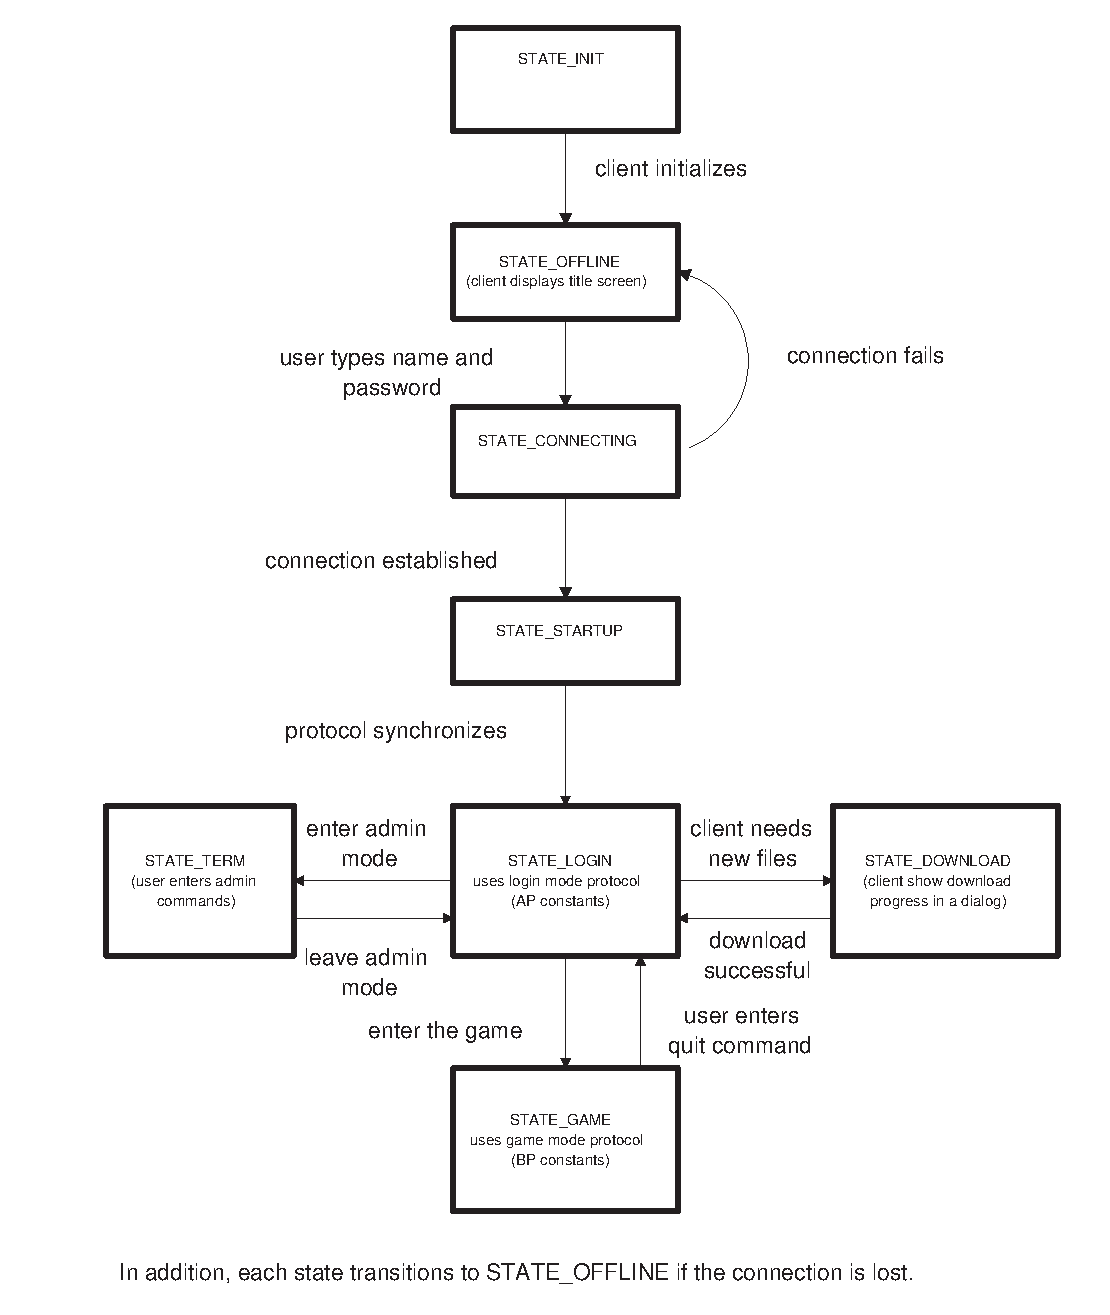
\epsfig{file=cstate1.eps}
\caption{State diagram for the client.}
\label{fig:state1}
\end{figure}

\begin{figure}
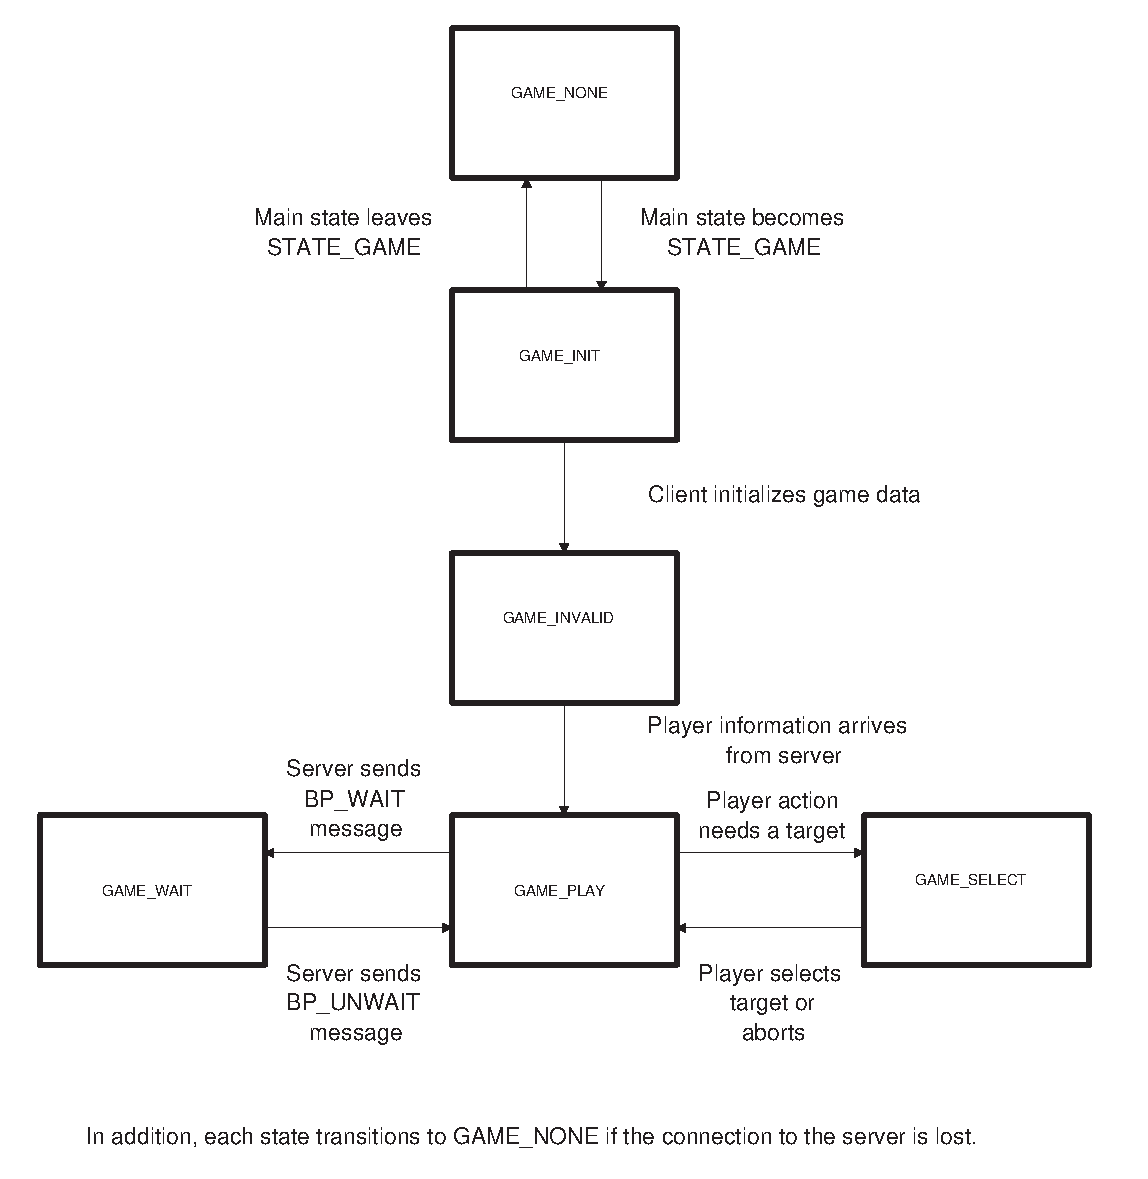
\epsfig{file=cstate2.eps}
\caption{State diagram for the client while it is in the main state
{\tt STATE\_GAME}.}
\label{fig:state2}
\end{figure}

\subsection{Memory usage}

The parts of the client that use the most memory are the frame
buffers, the current room's BSP tree, and the bitmap caches.

The main frame buffer is 452 by 276 pixels, and the larger buffer for
stretched images is twice as large in each direction.  Together, these
total 600 kilobytes of memory, which is allocated when the client
enters the game.

The size of the BSP tree in memory varies widely depending on the size
and complexity of the room.  Current rooms use up to approximately
300-400 kilobytes of memory.  

The client allocates most of free memory to bitmap caches, one for
textures, and one for all other bitmaps.  First the client determines
how much free virtual memory is available, and truncates this amount
at a maximum of 60 megabytes.  Then it estimates the size of the
operating system in memory, and sets aside 75\% of the remaining
amount for the object bitmap cache, and 25\% for the texture cache.
When a bitmap is loaded or accessed, it is added or moved to the front
of the cache's bitmap list; when the cache is full, bitmaps are
removed from the back of the list in least recently used order.

Other pieces that use substantial amounts of memory are the draw list
in the graphics engine, and Windows objects such as fonts, windows,
dialogs, etc.

%%%%%%%%%%%%%%%%%%%%%%%%%%%%%%%%%%%%%%%%%%%%%%%%%%%%%%%%%%%%%%%%%%%%%%%%%
\section{Dynamic updates}

Any part of the client installation can be dynamically updated, even
while the server is still running.  Updates are done via ftp using
Microsoft's Wininet DLL.  The ftp server machine need not be the same
as the game server machine; it is settable in the server's
configuration file.  To help transfers go faster, update files are
compressed with Crusher and decompressed after they are received.

Immediately after logging in, the client sends its version number to
the server.  If the client is out of date, the server tells the client
where to retrieve a new version.  The client then spawns a separate
program called {\tt club}, passing it the ftp server and filename to
download on the command line.  {\tt Club} retrieves the new client
version via ftp, decompresses it, and runs the new version.

The client's INI file contains a sequence number called the {\em
download time}, which identifies the latest data file update the
client has received.  When the client enters the game, it sends its
download time to the server; the server compares the time with the
value in its configuration file.  If the client's download time is
less than the server's configured value, the server sends instructions
on how to update the client's data files.  

On startup, the server reads a text file called {\tt packages.txt},
which contains a line for each action the client should take to update
its download time.  Each line of the file contains a download time, a
filename, and an integer which acts as flags, separated by spaces.
For each download time greater than the client's value, the server
sends these three fields in a message to the client.  The client
interprets the flags field as a particular action to take, and when
this action is complete, it updates the download time in its INI
file.  Assuming that all actions complete successfully, the client
tries to enter the game again; since its download time is now
synchronized to the server's value, it succeeds.

The flags field of a line in {\tt packages.txt} can instruct the
client to download or delete a file, and which directory the file
appears in.  The various flags values allow the client to update files
in any of its subdirectories, so that any data file can be updated.

One particular value of the flags field indicates that the client
should download a new banner advertisement graphic.  Normally, as the
client downloads files, it displays its progress in a dialog box to
the user.  However, to avoid giving the appearance that the game play
is being updated when only advertisements are changing, the client
instead displays a small message dialog as a decoy when all of the
files it needs to update are advertisements.

All of the settings related to updates in the server's configuration
file can be changed dynamically, and the {\tt packages.txt} can also
be edited and reloaded while the server is running.  Thus, any part of
the system can be updated without taking down the server.

%%%%%%%%%%%%%%%%%%%%%%%%%%%%%%%%%%%%%%%%%%%%%%%%%%%%%%%%%%%%%%%%%%%%%%%%%
\section{Security considerations}

Room and resource files are encrypted on client machines, so that
players cannot read or modify them.  Each room file also contains a
checksum that the client verifies when it loads the file, to make sure
it hasn't been modified.  As a final precaution, the client sends this
checksum to the server when it loads the room, and the server verifies
that the client has actually loaded the correct file.  This prevents
players from switching room files.  Other file types, such as
graphics, sound, and music, are stored unencrypted, because players
cannot gain an advantage by modifying them.

User passwords are run through the MD5 one-way hash function algorithm
before they are sent to the server; thus, passwords never appear in
plaintext on the network.  The server stores the hashed passwords in
its account file, so that even the theft of the account file will not
compromise any user accounts.

To prevent players from replaying packets, the protocol contains a
small amount of state.  When the client first connects, the server
sends it seeds for 5 pseudorandom number generators.  Each time the
client sends a message, it includes the output of one of the
generators.  The server verifies that the message contains the correct
pseudorandom number, and both the client and server synchronously
advance their generators.  Any client message that is either repeated
or blocked will be detected by the server.  Currently, when the server
detects such a mismatch, it simply writes the name of the offender to
its log file.

One way the system discourages snooping is by limiting the amount of
game information present on the client.  The world is divided into
rooms, and each client knows only which objects are present in the
same room as the player, as well as the positions and names of these
objects.  The client also has knowledge of the entire map of the room,
and the names of all players who are logged in.  Even armed with all of the
game data present in the client, a player would not have much of an
advantage.  All object data is stored on the server, and only reaches
the client through a restrictive set of messages.

Using the administrator mode, it is possible to gain complete control
over a server.  The client only accepts administrator mode commands
when the server grants it permission; however, it would be possible
for an attacker to modify the client to get it to display
administrator mode.  For this reason, the server verifies each
incoming administrator command, to make sure that its associated
account actually has administrator privileges.  Using administrator
mode thus requires knowledge of an administrator account's password,
or physical access to the server machines.

There are no known security holes in the current scheme.  In order to
cheat, a player would have to reverse the MD5 algorithm, discover the
password to the Crusher encryption scheme or break the scheme,
discover and reproduce the random packet state algorithm, or modify
the client executable.  Even by modifying the client executable, it is
only possible to discover a relatively small amount of information
about the player's local area.

\newcommand{\class}[1]{\textbf{#1}}
\newcommand{\prop}[1]{\texttt{#1}}

\newenvironment{leftlines}
{\setlength{\oldindent}{\parindent}
 \setlength{\parindent}{0in}\vspace{\baselineskip}}
{\setlength{\parindent}{\oldindent}\vspace{\baselineskip}}

\newcommand{\function}[2]{ {\tt #1(} {\em #2} {\tt )} }

\chapter{The Blakod language}

Blakod is the language that BlakSton uses to define objects in its
game world.  BlakSton contains a byte compiler from Blakod to an
simple intermediate language, and an interpreter for the intermediate
language.  This chater informally describes the syntax and semantics of
Blakod.  

Blakod is an object-oriented language that uses message passing as a
primary means of flow control.  An object consists of some private
data, called {\em properties\/}, and a set of methods (which we refer
to as {\em message handlers\/}) for observing and manipulating this
private data.  The syntax of the language is much like that of
C or Pascal.  

Because Blakod is a special-purpose language, meant to describe
objects for use in role-playing games, there is a close relationship
between the Blakod written for a game and the runtime system in the
BlakSton server.  Blakod code calls built-in C functions in the server
when an operation would be too slow or complicated in Blakod, or where
the operation requires communication with other parts of the server,
such as sending messages to clients running on user machines.

%%%%%%%%%%%%%%%%%%%%%%%%%%%%%%%%%%%%%%%%%%%%%%%%%%%%%%%%%%%%%%%%%%%%%%%%%
\section{Specification}

A Blakod code file contains definitions for one or more classes.  Each
class definition consists of six parts, as illustrated in
figure~\ref{fig:class}.  The class header lists the name of the class,
and optionally the name of a single superclass.  Only single
inheritance is allowed.


\begin{figure}

\begin{verbatim}
Classname is Superclass                      % Class header

constants:                                   % Constant block

  include constants.khd
  seconds_per_hour = 3600

resources:                                   % Resource block

  filename = picture.bmp
  string = "Text goes here"

classvars:                                   % Class variable block

  ciBitmap = filename

properties:                                  % Property block

  piWeight = 10

messages:                                    % Message block

  Move(distance = 1, direction = 1)
  "This message handler moves this object in some way."
  "And these comments can extend over multiple lines."
  {
    local i, j;
    ...
  }

end
\end{verbatim}

\caption{Basic format of a Blakod class}
\label{fig:class}

\end{figure}

The constant block lists identifiers to be used as abbreviations for
simple constant expressions.  Such an identifier evaluates to the
right hand side of the assignment given in the constant block wherever
it appears.  The constant block can also contain {\tt include}
compiler directives that can be used to include a set of constant
definitions from other files.

Identifiers in the resource block reference filenames and strings.  A
class's resources are placed in a resource file during compilation,
and this file is sent to clients.  Each resource is assigned a unique
number during compilation, and it is these numbers that the server
uses to refer to files and strings in messages to the client.  In
Blakod, resources can only be passed as parameters or appear by
themselves on the right hand side of assignments; they cannot be
assigned to or appear in compound expressions.

Properties are the equivalent of protected class data in C++.  A class
inherits all the properties of its direct and indirect superclasses;
these properties are all accessible within the class.  Properties of a
superclass can appear in the subclass's property section in order to
override the superclass's values for these properties.

A class variable is a piece of read-only, per-class data.  Class
variables are inherited by subclasses just as properties are.  The
main use of class variables is to save space in the object database;
data that doesn't vary across instances of a class should be put in
class variables to avoid allocating space in each object for the
data.

A subclass can overload a superclass's class variable by declaring a
property with the same name.  The subclass can then use the property
as read-write data just like any other property.  In this way, a class
high in the hierarchy can declare read-only data to save space in most
objects, while subclasses can still write to the location if they need
to (though instances of the subclass will of course require extra
space to hold the property).

Properties and class variables can be initialized to any constant
expression.  If no expression is given, they are initialized to the
special value nil.

The message block contains the class's message handlers.  Each message
handler begins with a header that lists the handler's name and
parameters.  Parameters are matched by name, so that calls of a
handler need not assign values to all of the parameters listed in the
handler's header.  The header can list default values for any of its
parameters; a default value is bound to its parameter when a call does
not list the parameter.  The header is optionally followed by a
comment, describing the message handler.  Administrators can view
these comments in the game.

A message handler's body contains a sequence of statements, each
ending with a semicolon.  The first statement optionally declares a
list of local variables used by the handler.  A class also inherits
its superclass's message handlers.  When an object's class hierarchy
contains more than one message handler of the same name, the handler
for the lowest class in the object's hierarchy is called first.  This
handler can propagate the message to the next handler up the
hierarchy, or it can return a value, in which case the other handlers
are not called.

A special message handler called {\tt Constructor} is called when an
object is created.  Right before an object's constructor is invoked,
its default property values are set in descending class order,
starting with the top of the object's class hierarchy and ending with
the object's actual class.  This is the reverse order of the message
handler call sequence, allowing subclasses to override property values
of superclasses.

Some objects call the message {\tt Constructed} in their constructor.
This is no longer needed, but at one time was done to allow certain
processing after the {\tt Constructor} message was propagated
all the way up to the {\tt Object} class.  Since {\tt Object}'s
constructor now does very little, {\tt Constructed} is no longer necessary.

Class and message handler names have global scope. Each class name
must be globally unique, and message handler names must be unique
within a class.  The scope of all identifiers appearing on the left
hand sides of assignments in the constant, resource, property, and
classvar blocks is the class in which the blocks appear.  Parameter
names and local variables appearing in a message handler have scope
restricted to that message handler.

\subsection{Statements and expressions}

Blakod statements correspond roughly to similar statements in C.  The
main differences are due to Blakod's dynamic type scheme, and message
handler calls.

Values in Blakod are 32 bits long; 4 of these bits act as a tag that
determine the value's type.  Thus, 28 bits are actually available to
the program\footnote{With one sign bit, this means that $2^{27} - 1
\approx $
134 million is the largest number expressible in a single Blakod
variable.}.  Blakod can directly express values of type integer,
resource, class, message handler, and nil.  There is no non-integer
numerical type.  The interpreter uses other tag values for runtime
types such as objects and list cells.  Type checking is done at
runtime; thus, expressions with type errors will compile but may cause
runtime errors.

The special value nil is denoted by a dollar sign ({\tt \$}).  Nil is
assigned to message handler parameters that are not explicitly
assigned a value, and it is also used to mark the end of a list.  Nil
can be assigned to variables, returned from message handlers, or
tested for equality; it is an error to perform any other operation on
nil.

The special value {\tt self} contains the identifier of the object
whose message handler is being executed.  {\tt Self} is implemented as a
property of every object.

Expressions consist of identifiers, constants, and message handler
calls combined with standard operators.  Blakod contains the following
operators: addition, subtraction, multiplication, division, unary
minus, modulo, logical and bitwise AND, OR, and NOT, and the standard
relational operators (equal, less than, etc.).  A boolean expression
evaluates to 0 if it is false, or nonzero if it is true.  The logical
AND and OR operators ``short-circuit;'' i.e. they only evaluate their
second arguments if necessary.  The following table shows the
precedence of Blakod operators in descending order.

\begin{center}
\begin{tabular}{|l|}
\hline
$-$ NOT $\sim$ \\
$*\ /$\ MOD \\
$+ -$ \\
$<\  >\ <=\ >=\ =\ <>$ \\
\& \\
$\mid$ \\
AND \\ 
OR \\
\hline
\end{tabular}
\end{center}


Blakod programs are made up of assignment statements, conditional
clauses, loops, calls, and return statements.  Comments are introduced
by the percent character ({\tt \%}) and extend to the end of the
line.

Assignments take the form {\em lvalue} {\tt =} {\em expression}, where
{\em lvalue} is the name of a property or a local variable.  The right
hand side is evaulated, and the result is assigned to the left hand
side.

The {\tt if} statement performs conditional execution.  Its syntax is
\begin{center}
{\tt if} {\em test} {\tt \{} {\em then-clause} {\tt \}} or
\linebreak
{\tt if} {\em test} {\tt \{} {\em then-clause} {\tt \} else \{} {\em
else-clause} {\}}.
\end{center}
The braces are required in all cases.

The basic looping construct in Blakod is the {\tt while} loop.  A while
statement has the syntax 
\begin{center}
{\tt while} {\em loop-test} {\tt \{} {\em loop-body} {\tt \}}.
\end{center}
The loop body is evaluated until the loop test becomes false (equal to
zero).  The {\tt for} loop construct is for use with lists only.  Its
syntax is
\begin{center}
{\tt for} {\em loop-var} {\tt in} {\em list} {\tt \{} {\em loop-body} {\tt \}}.
\end{center}
The loop variable takes on each of the first values of the list during
evaluation of the body of the loop.  The {\tt break} and {\tt
continue} statements can be used to interrupt loop execution as in C.
These statements apply to the innermost enclosing loop; it is an error
for these statements to appear outside a loop.

Function calls may appear either as expressions, in which case they evaluate
to the return value of the function they call, or as statements, in
which case the return value is ignored.  The most important call is
{\tt Send}, which calls an object's message handler.  The syntax is
\begin{center}
{\tt Send(} {\em object, } {\tt @}{\em message}, {\tt \#}{\em param1}
{\tt =} {\em val1}, {\tt \#}{\em param2} {\tt =} {\em val2}, \ldots
{\tt )}
\end{center}
{\em Object} gives the object whose message handler is to be called;
{\em message} is the name of the message handler to call.  The
parameters are matched by name, so they can appear in any order.
Execution immediately passes to the object's message handler, and
returns to the caller when a return statement is reached in the
handler.  All parameters do not need to be supplied.  Any parameters
not passed to a message handler are initialized to the value specified
in the message handler definition before the message handler code
gets control.

\texttt{Post} has the same syntax as \texttt{Send}, but the
call is not made until after the current message (and all of the
callers, back to the original client message forwarded by the server)
is complete.  This is useful when something should be done after the
current call, such as responding to speech said by a user.

There are two kinds of return statements, {\tt return} and {\tt
propagate}.  One of these must be the last statement in every message
handler.  A {\tt propagate} statement indicates that execution should
proceed to the message handler of the same name in the closest
superclass in the current class's hierarchy, if any.  A {\tt return}
statement indicates that execution should return immediately to the
caller.  {\tt Return} can optionally be followed by an expression
whose value is returned to the caller as the value of the calling
expression.  If no expression appears after the {\tt return}, the
value nil is returned to the caller.

Debug strungs are a special kind of string that is only intended for
debugging use.  They are specified by a text string inside
double quotes in an expression.  The primary use for debug strings
is to pass them to the {\tt Debug} function, described in the next section,
for output to a log file.  However, they can also be used as parameters
to {\tt StringEqual} and {\tt ParseString} for use in text comparisions
and in parsing mail destination lists.  Debug strings are not handled
by the other string functions, so care must be taken not to use debug
strings where they are not appropriate.

\subsection{Built-in functions}

Below we give brief descriptions of each built-in function, arranged
by category.  All parameters are passed by value.  A more thorough description 
is given in the previous chapter.

\subsubsection{List operations}

These functions support linked lists similar to those in Lisp.  The
interpreter has a linked list data type; values of this type are
passed as list arguments to these functions, and appear in {\tt for}
statements.

\newlength{\oldindent}

\begin{leftlines}
\function{Cons}{expr1, expr2}

\function{First}{list node}

\function{Rest}{list node}
\end{leftlines}

Same as their Lisp counterparts.  {\tt Cons} creates a ``dotted pair'' of
its arguments, which we refer to as a {\em list node}.  {\tt First}
and {\tt Rest} return the first and second parts of a list node.

\begin{leftlines}
\function{List}{expr1, expr2, \ldots}
\end{leftlines}

Create a list of its arguments.  A list is a sequence of list nodes,
where the first element of the $n^{th}$ node contains the value of the
$n^{th}$ expression, and the second element contains a reference to
the $(n+1)^{st}$ node.  The second element of the last node contains
nil.

A call to {\tt List} can be abbreviated by the syntactic sugar {\tt [}
{\em expr1, expr2,} \ldots {\tt ]}.

\begin{leftlines}
\function{Nth}{list, n}
\end{leftlines}

Return the first element of the $n^{th}$ node in the list.

\begin{leftlines}
\function{SetFirst}{list}

\function{SetNth}{list, n}
\end{leftlines}

Mutate the first element of the $n^{th}$ node of {\em list} in place, that is, without
creating any new list nodes.  SetFirst is a special case with $n = 1$.

\begin{leftlines}
\function{Length}{list}
\end{leftlines}

Return the length of the given list.

\begin{leftlines}
\function{DelListElem}{list, n}
\end{leftlines}

Returns the list with the first occurrence of the specified value ($n$) 
removed from the list.


\subsubsection{Communication}

These commands assemble and send messages that the interpreter passes
to the client.

\begin{leftlines}
\function{AddPacket}{expr1, expr2, \ldots}
\end{leftlines}

Add to the interpreter's communication queue.  The first argument
gives the length of the second argument in bytes, the third argument
gives the length of the fourth argument, etc.  The communication queue
contains everything passed in via calls to {\tt AddPacket} since the
last call to {\tt SendPacket}.

\begin{leftlines}
\function{SendPacket}{session}

\function{SendCopyPacket}{session}

\function{ClearPacket}{}
\end{leftlines}

Send the contents of the communication queue to the client identified
by {\em session}, and then clear the queue.  The interpreter passes
session numbers to Blakod when users log on.

{\tt SendCopyPacket} performs the same function, except that it
doesn't clear the queue.  The queue can be cleared manually by calling
{\tt ClearPacket}.

\subsubsection{Class operations}

\begin{leftlines}
\function{Create}{{\tt \&}class, {\tt \#}param1 {\tt =} val1, {\tt \#}param2 
{\tt =} val2, \ldots}
\end{leftlines}

Create and return a new object of the given class.  The parameters are
passed to the class's constructor.

\begin{leftlines}
\function{IsClass}{object, {\tt \&}class}
\end{leftlines}

Return true if the object is a subclass of the given class.

\begin{leftlines}
\function{GetClass}{object}
\end{leftlines}

Return the class of the given object.


\subsubsection{Strings}

\begin{leftlines}
\function{StringEqual}{string1, string2}
\end{leftlines}

Return true if the two strings contain the same ASCII string; the
comparison is case insensitive.

\begin{leftlines}
\function{StringContain}{string1, string2}
\end{leftlines}

Return true if the string1 contains the ASCII string in string2; the
comparison is case insensitive.

\begin{leftlines}
\function{SetString}{string1, text}
\end{leftlines}

Set the string to the given ASCII text.

\begin{leftlines}
\function{SetResource}{resource, string}
\end{leftlines}

Set the dynamic resource to the given string.

\begin{leftlines}
\function{CreateString}{}
\end{leftlines}

Create a new, empty string.

\begin{leftlines}
\function{ParseString}{string, separators, message}
\end{leftlines}

Parse the given string into a set of substrings, separated by
characters in the string {\tt separators}.

\subsubsection{Timers}

\begin{leftlines}
\function{CreateTimer}{time, message}
\end{leftlines}

Create and return a new timer.  The timer will go off in {\tt time}
milliseconds, when the given message will be sent to the current object.

\begin{leftlines}
\function{DeleteTimer}{timer}
\end{leftlines}

Delete the given timer.

\begin{leftlines}
\function{GetTimeRemaining}{timer}
\end{leftlines}

Return the number of milliseconds remaining on the given timer.

\begin{leftlines}
\function{GetTime}{}
\end{leftlines}

Return the current wall clock time.

\subsubsection{Room operations}

\begin{leftlines}
\function{LoadRoom}{expr}
\end{leftlines}

Return a reference to the room description given by the resource
number {\em expr}.  This function is used to load the room's
description file when the room is created.  The data that BlakServ loads
about a room is nearly permanently stored in memory.  It is only unloaded
upon a {\tt reload sys} command, which unloads the data about every loaded
room.  The Blakod for every game must reload rooms after every system
reload, and also erase all references to the room data that no longer
exists.  I coded Meridian 59 to automatically take care of this through
the {\tt Room} class, and it is important not to remove that code.  Other
games may not need rooms at all, and can ignore this warning.  There is no
way to unload room data except by a system reload.

\begin{leftlines}
\function{CanMoveInRoom}{room, row1, col1, row2, col2 }
\end{leftlines}

Return true if room does not contain any impassable walls when moving
from ({\em row1, col1}) to ({\em row2, col2}).  This is used to
determine if monster moves should be allowed.  This is currently the
only interaction between Blakod and the geometry of a room.

\subsubsection{Hash tables}

\begin{leftlines}
\function{CreateTable}{}
\end{leftlines}

Return a new, empty hash table.  The ``size'' of the table is fixed in {\tt ccode.c},
but the hash table uses open hashing.  Open hashing is a very common
hashing system which is quite simple.  Each entry in a hash table is
actually a linked list of elements that have the same hash value.  In
this way, the hash table is never full, because it is not of a fixed size,
just a fixed number of hash values.  This considerably eases coding using
a hash table because the programmer never has to deal with a full hash table.
However, implementing open hashing is slightly more complex.  I believe that
the hash tables work perfectly in BlakServ.


\begin{leftlines}
\function{AddTableEntry}{table, key, value}
\end{leftlines}

Add the (key, value) pair to the given hash table.

\begin{leftlines}
\function{GetTableEntry}{table, key}
\end{leftlines}

Return the value matching the given key in the hash table, or nil if
the key is not present in the table.

\begin{leftlines}
\function{DeleteTableEntry}{table, key}
\end{leftlines}

Remove the entry in the hash table with the given key, if any.

\begin{leftlines}
\function{DeleteTable}{table}
\end{leftlines}

Free all memory associated with the given hash table, and delete the
table.

\subsubsection{Miscellaneous}

\begin{leftlines}
\function{Random}{expr1, expr2}
\end{leftlines}

Return a random number uniformly distributed over the given closed
interval of integers.

\begin{leftlines}
\function{Debug}{expr1, expr2, \ldots }
\end{leftlines}

Print given values on the server's terminal.

\begin{leftlines}
\function{Bound}{expr1, expr2, expr3 }
\end{leftlines}

Bound {\em expr1} to the interval [{\em expr2, expr3}], and return
the result.

\begin{leftlines}
\function{Abs}{expr}
\end{leftlines}

Return the absolute value of the given expression.

\begin{leftlines}
\function{GetInactiveTime}{session}
\end{leftlines}

Return the number of milliseconds since a message was received on the
given session.

\begin{leftlines}
\function{IsList}{object}
\end{leftlines}

Return true if the object is a list node.

%%%%%%%%%%%%%%%%%%%%%%%%%%%%%%%%%%%%%%%%%%%%%%%%%%%%%%%%%%%%%%%%%%%%%%%%%
\section{Intermediate language}

Blakod is byte-compiled into an intermediate language we call Bkod.
Bkod is an extremely simple language, similar to a generic
register-oriented assembly language.  Each instruction contains an
opcode, one to three sources or destinations, and occasionally some
other fields. For a full specification, see Appendix~\ref{app:formats}.

Bkod contains opcodes for unary and binary operations, jumps, function
calls, and returns.  The unary and binary operations have the same
semantics as C (except, of course, that they operate on Blakod's 28
bit values).  Jumps may be conditional or unconditional, and returns
may or may not propagate (corresponding to the Blakod commands {\tt
propagate} and {\tt return}).

The only locations allowed in Bkod instructions are local variables
and properties.  Temporary values, such as values that arise in the
evaluation of complex expressions, are stored in extra local variables
generated by the compiler.  Immediate (constant) values can also
appear in Bkod instructions.

In addition to instructions, a \bof file contains some organizational
information about the class from which it was compiled.  The class has
a table of message handlers; each handler contains a list of its
parameters, as well as the actual handler's Bkod instructions.  The
file also contains a mapping of \bof file offsets to source (Blakod)
line numbers; the server uses this to report Blakod line numbers in
debugging messages.

%%%%%%%%%%%%%%%%%%%%%%%%%%%%%%%%%%%%%%%%%%%%%%%%%%%%%%%%%%%%%%%%%%%%%%%%%
\section{Existent Blakod}

\subsection{Class Hierarchy}
As of the date of this writing, the following class tree shows the
class hierarchy of the Blakod, except for the leaves.  In most
cases leaf classes have little or no added functionality.  Their only
purpose is to have resources for the individual object and use these
to override properties.

\begin{verbatim}
Object*
    ActiveObject*
        Holder*
            NoMoveOn*
                Battler*
                    Monster*
                        Council
                        Factions
                        Mummy
                        Temples
                        Towns
                            BarloqueTown
                            CorNothTown
                            HazarTown
                            JasperTown
                            MarionTown
                            TosTown
                    Player
                        User
                            dm
                                admin
            Room*
                Guest1
                Guest2
                Guest3
                Guest4
                Guest5
                Guest7
                GuildHall
                MonsterRoom
                    FeyForest
                    Guest6
                    ObjectRoom
    Item*
        ActiveItem*
        PassiveItem*
            AttackModifier
            DefenseModifier
                Armor
                Helmet
                Pants
                Shield
            ForgetPotion
            Healer
            MiniGame
            Necklace
            NumberItem
                Ammo
                Food
            Ring
            Token
            Wand
            Weapon
                RangedWeapon
    PassiveObject*
        Brain*
        GuildCommand
        ManaNode
        News
        Sickness
            Disease
        Skill
            Proficiency
            Stroke
                Unarmed
        Spell
            AttackSpell
            DMSpell
            TouchAttackSpell
        TreasureType
UtilityFunctions*
    System* (an important leaf class)
\end{verbatim}
* infrastructure class

\begin{center}
Non-leaf classes in the class hierarchy
\end{center}

\subsection{Some important classes}

\subsection{Holder}

The \class{Holder} class is critical to the function of the system in
many ways.  See the following table for its properties.

\begin{center}
\begin{tabular}{||l|l||} \hline
Property name & Description 
\\ \hline \hline
\prop{plActive} &  A list of active objects being held by this object.
\\ \hline
\prop{plPassive} &  A list of passive objects being held by this object.
\\ \hline
\prop{piBulk\_hold} &  The amount of bulk this object is currently holding.
\\ \hline
\prop{piWeight\_hold} &  The amount of weight this object is currently holding.
\\ \hline
\end{tabular}
\end{center}

The \class{Holder} class uses the concept of active and passive
objects.  When an \class{Holder} class receives a message indicating
something has happened or might happen, it sends this message to all
the active objects that it holds.  This is the primary way that
objects learn about what is going on with other objects, and how they
affect other objects.

Many of the messages come in pairs.  This is because an object first
checks to see if it can do something (such as cast a spell), and then if
nothing prevents it, it actually performs the action.  The most important
of these messages are summarized in the following table.

\begin{center}
\begin{tabular}{||l|l||} \hline
Message name & Description 
\\ \hline \hline
ReqSomethingUse &  An object would like to use an item.
\\ \hline
SomethingUse  &  An object just used an item.
\\ \hline
ReqSomethingMoved &  An object would like to move.
\\ \hline
SomethingMoved &  An object actually did move.
\\ \hline
ReqSpellCast &  An object would like to cast a spell.
\\ \hline
SpellCast    & An object just cast a spell.
\\ \hline
SomethingChanged &  An object just changed its look (either bitmap or overlays).
\\ \hline
\vdots & \vdots
\\ \hline
\end{tabular}
\end{center}

The idea here is that rooms have no owner, but every other object is
either directly owned by a room or owned by an object which is owned
by a room, some levels up.  When something happens in a room, every
active object in the room is sent a message, and any of these objects
which are holders forward the message to any active objects they are holding.

\subsubsection{Room}

The \class{Room} class derives from the \class{Holder} class, but adds
essential features to store object coordinates and a few other things.
Its properties are listed in the following table.
\begin{center}
\begin{tabular}{||l|p{4in}||} \hline
Property name & Description 
\\ \hline \hline
\prop{piRoom\_flags} & Specified properties of a room---whether it is
a no combat zone, whether it is an anti-magic zone, etc.
\\ \hline
\prop{prRoom} &  The resource of the room filename (.roo file)
\\ \hline
\prop{prmRoom} &  The server room id  returned by the server when the .roo
file \\
               &  is loaded each time the server is started (or reloaded).
\\ \hline
\prop{piRoom\_num} &  The room id for this room, which is unique for
each room \\
	         &  (constants have prefix RID\_)
\\ \hline
\prop{piSecurity} & The security value of the .roo file associated with
this room, retrieved from the server.
\\ \hline
\prop{prMusic} &  The resource of the midi file to play for users in
this room.
\\ \hline
\prop{piNorth} &  The room id of the room to send objects to if they
leave to the north.
\\ \hline
\prop{piSouth} &  The room id of the room to send objects to if they
leave to the south.
\\ \hline
\prop{piEast} &  The room id of the room to send objects to if they
leave to the east.
\\ \hline
\prop{piWest} &  The room id of the room to send objects to if they
leave to the west.
\\ \hline
\prop{piBaseLight} &  The base light level in this room (constants
have prefix LIGHT\_).
\\ \hline
\prop{piOutside\_factor} &  How much this room's light is affected by
time of day \\
                   & (constants have prefix OUTDOORS\_).
\\ \hline
\prop{piDirectional\_percent} & How effective directional light is in this room.
\\ \hline
\prop{piDirectional\_light} & An internal measure of directional light calculated
over time.
\\ \hline
\prop{prBackground} & The resource of the background bitmap of this room.
\\ \hline
\prop{piDispose\_delay} &  The amount of time between sending
DestroyDisposable() messages.
\\ \hline
\prop{ptDispose} &  The timer id returned by the server when a timer
is created to call DestroyDisposable().
\\ \hline
\prop{plExits} & The list of exits from this room (accessed by a user hitting
the space bar).
\\ \hline
\prop{plSector\_changes} & The list of all sectors that have a changed floor or
ceiling height from the .roo file height.
\\ \hline
\prop{plWall\_changes} & The list of wall ids that have a different animation
type from the .roo file value.
\\ \hline
\prop{plTexture\_changes} & The list of wall texture ids that have been assigned
a different texture from the .roo file value.
\\ \hline
\prop{plSector\_light\_changes} & The list of sectors that have a different
light value from the .roo file value.
\\ \hline
\prop{plEnchantments} & The list of all room enchantments that are currently
affecting this room.
\\ \hline
\end{tabular}

\begin{tabular}{||l|p{4in}||} \hline
Property name & Description 
\\ \hline \hline
\prop{pbUser\_in\_room} & Internally calculated.  True when there is at least
one user in the room.
\\ \hline
\prop{plPeriodic\_sounds} & The list of all sounds that are set to periodically
be sent to all users in the room.
\\ \hline
\prop{piPeriodic\_sounds} & The number of milliseconds between periodic sounds
going off.
\\ \hline
\prop{ptPeriodic\_sounds} & The timer that goes off when a new periodic sound is
set to be sent to all users in the room.
\\ \hline

\end{tabular}
\end{center}

An object of class \class{Room} stores the angle, row, column, fine
row, and fine column of each object it is holding in the
\prop{plActive} and \prop{plPassive} lists, besides the actual object.

The \class{Room} class keeps track of when the first user enters the
room and when the last user leaves.  The room itself uses this to send
all the objects in the room a \texttt{DestroyDisposable()} when the
user leaves, or every \prop{piDispose\_Delay} seconds when users are
present.  Objects which are not permanent should delete themselves
upon receiving this message.  Items by default do this, as do
monsters.  Any ``permanent'' items or monsters override this behavior.

\subsubsection{Monsters}

The \class{Monster} class has a simple system of fighting, by
returning attacks by anything that attacks a monster, and retaliating
by a timer.  It has properties to keep track of its hit points and
damage capabilities, and to create treasure when it is killed.

This class was originally written by Chris Kirmse, but was rewritten
by John Murphy; he and Damion Schubert understand its behavior best.

\subsection{Users}
\label{section:users}

The code and data to handle users is split primarily into two classes,
\class{Player} and \class{User} (which derives from \class{Player}).
The \class{Player} class handles attacking, using and holding items,
and animations and overlays.  The \class{User} class handles all the
interaction with the server (which comes through the message handler
ReceiveClient()).

\subsubsection{Using items}

The \class{Player} class allows users to use items.  Items may be used
in several different ways, as seen in table~\ref{tabconstantsuse}.

\begin{center}
\begin{center}Table \ref{tabconstantsuse} \end{center}
\begin{tabular}{||l|l||} \hline
Value of item's \prop{piUse\_type} & Description 
\\ \hline \hline
ITEM\_CANT\_USE &  The item cannot be used.
\\ \hline
ITEM\_SINGLE\_USE  &  The item does something when used, like a
magical staff or bandage.
\\ \hline
ITEM\_USE\_HAND &  The item is held in a hand.
\\ \hline
ITEM\_USE\_BODY &  The item is held on the body.
\\ \hline
ITEM\_BROKEN    &  The item is broken, and so cannot be used.
\\ \hline
\end{tabular}
\label{tabconstantsuse}
\end{center}

Each user has an amount of \emph{space} to hold things in his hands or on
his body, stored in \prop{piHand\_space} and \prop{piBody\_space}.  If
the amount of space is greater than the amount the item will use
(specified in its \prop{piUse\_amount}), then there is enough space to
use the item.

Items themselves may have other restrictions on usage--for example,
only one weapon may be used at a time, and if a user tries to use
another weapon, the currently used weapon will ``unuse'' itself.


\section{Strings and dynamic resources}

\subsection{How player names work}

Player names presented quite a challenge to us early on in BlakSton, but
after several tries we came up with a good solution.  The problem is that
Blakod refers to all object's names as resources.  This makes it possible
for a piece of Blakod to deal with all objects the same--there is no special
case code for users.  However, players need the ability to change their
name (when they create their character the first time, and any time they
commit suicide).  Additionally, player names are not known before the
game is shipped, which is the case for all other resources.

The solution currently implemented in BlakSton is that player names are
treated as special resources, called \textit{dynamic resources}.  All resources
with resource ids of at least 1 million are treated as dynamic resources.
Unlike regular resources, when the server saves the game state, it also saves
all of the dynamic resources.  A C code function (\texttt{SetResource}) exists
for the Blakod to change a player's name.  The only remaining issue is how to
make sure all clients always know the dynamic resources associated with every
player currently logged in.

This is simple to accomplish--when a player logs in, all other players are sent
a special message from the server with the new player's name resource id and 
the string value of the resource.  The new player is sent a message with
every logged in player's resource ids and associated strings.  In this way,
all clients always know the string values of all static resource ids and
all dynamic resource ids of currently logged in players.

\subsection{How strings and dynamic resources are saved}

When the server saves the game state, it writes several files with a suffix
indicating the time of the save.  One of these files is called \texttt{dynarscs.X},
which contains the dynamic resources in the same format as a \texttt{.rsc} file.
When the game is reloaded, the server reads the file and so never loses track
of player names.

The game strings are saved to a file called \texttt{striings.X}, which is in
a very simple binary format.  It starts with the bytes 00, 00, 00, 01.  Then
the number of strings is written as a four byte integer in little endian format.
Then each string is written to the file, as a two byte integer length and then
the actual string data.

\chapter{Tools}

This chapter describes the parts of the system other than the server
and the client.  This is mainly a guide to using these standalone
programs, since their design is for the most part trivial.  However,
in the discussion of the Blakod compiler, we touch on some of the
implementation issues of Blakod that are separate from the
specification of the language.  In the section on the room editor, we
also explain some of the structures that are used in the client's
graphics engine to describe a scene.

\section{Blakod compiler ({\tt bc})}
\label{sec:compiler}

The Blakod compiler is a command line program that byte-compiles a
Blakod source (\kod file) into an object file (\bof file), and usually a
resource file (\rsc file).  The Blakod interpreter in the server loads all
\bof files at startup, while the \rsc files are sent to clients.

Link errors are appended to a file called kodbase.txt with a lowercase
letter and an identifier to indicate unresolved linkages.  The
lowercase letter indicates the type of the identifier that was
unresolved (property, class, message handler, or class variable).
This results in ``unrecognized character in kodbase.txt'' messages in
the server status window if this kodbase.txt file is loaded.  To
resolve these messages, the link error in Blakod must not only be
corrected, but the error message at the end of kodbase.txt must be
manually deleted.  The compiler will not remove these error messages,
even after the link error is resolved.

\subsection{Design of the compiler}

The Blakod compiler follows traditional compiler design, with separate
components for lexing, parsing, code generation, and optimization.  It
links with the {\tt flex} and {\tt bison} programs, which are GNU
versions of the UNIX utilities {\tt lex} and {\tt yacc}.  These
utilities take as input simple descriptions of Blakod's tokens and
grammar, and produce as output the parser component of the compiler.

The parser checks the input Blakod source for errors, and converts it
to an internal representation.  At the top level, this representation
consists of a list of the classes present in the source file.  Each
class holds a list of component resources, class variables,
properties, and message handlers.  Finally, each message handler
contains a parameter list, information on its local variables, and a
list of statements.  Expressions within statements are represented as
standard inorder expression trees, with operators at the nodes and
values at the leaves.

As the parser encounters new identifiers, it inserts them into a
global symbol table.  This provides a rudimentary type checking,
preventing, for example, a local variable and a parameter to share the
same name.  The symbol table records the string name of each
identifier, as well as a number that the object file will use to refer
to the identifier.  The parser adds the names of built-in Blakod
functions to the symbol during initialization; these use well-known
identification numbers so that the server can tell which built-in
function is being called by a particular statement.

If the parser encounters errors, these are reported and compilation
stops.  If there are no errors, the code generator recursively
traverses the code tree and produces \bof intermediate language
statements for each Blakod statements, and writes these out to disk.
Finally, the resources for all the classes present in the input source
file are placed in a \rsc file and encrypted.  Encryption is necessary
to keep users from reading strings which might give them an advantage
in game play.  If no resources are present, the \rsc file is not
generated.

The compiler performs the single optimization of constant folding;
that is, constant expressions are replaced by the resultant value of
the expression.  This optimization is important because it improves
code readability: bitwise constant combinations and complicated
formulas can be expressed simply without impacting performance.  Upon
reaching an expression, the code generator calls the optimizer to
simplify the expression if possible; the simplified expression
replaces the original form.

Because there is no linker, references to identifiers in other classes
must be stored externally.  A text file named {\tt kodbase.txt} keeps
track of all identifiers in previously compiled classes.  Each line in
{\tt kodbase.txt} contains an identifier's text string, the
identifier's compiler-generated number that appears in object files,
and a letter indicating the identifier's type---either class, message
handler, class variable, resource, property, parameter, or the special
value ``missing.''  The missing value is for forward references, that
is, identifiers that the compiler encounters before it can determine
type information.  The compiler will replace the missing value with
the identifier's type when it can be determined from another source
file.

The compiler loads {\tt kodbase.txt} upon startup, and writes it out
again after code generation.  In addition to substituting for a
linker, the file is used by the server in two ways.  First, saved
games reference identifier names, so that a saved game can be reloaded
even if all identifier numbers change.  Second, identifier names are
used in administrator mode for user convenience.

Saved games can be reloaded even if all identifier numbers change,
since saved games reference the names, not the numbers.  Rebuilding
the Blakod with working off the same kodbase.txt and hence the same
reference numbers will still allow the server to reload saved games.
To rebuild all the Blakod, you should first delete all the compiled
bof files.

The compiler supports an {\tt include} directive that inserts one
source file in another.  Though this directive may appear anywhere, it
is typically used to include global constants in the {\tt constants}
section of a class declaration.  {\tt include}s may be nested to a
depth of 10.

\subsection{Running the compiler}

The compiler is a console mode Win32 program named {\tt bc.exe}.  Its
simplest invocation is

{\tt bc} {\em input\_filename}{\tt .kod}

\noindent
which compiles the input file to output files with {\tt .bof} and {\tt
.rsc} extensions.  The command line switches are

\begin{tabular}{ll}
{\em -d} & include debugging information in the \bof file (see the
description \\
	& of the \bof file format in Appendix~\ref{app:formats}).
\\
{\em -K filename} & use {\em filename} as the kodbase file.
\\
{\em -I path} & look for included files in the {\em path} directory.
\end{tabular}

If compilation completes without errors, the compiler exits with the
value 0; otherwise, it exits with a nonzero value.  The build system
uses this return value to know when to terminate.

In \bof files, properties are identified by number.  The {\tt
kodbase.txt} file is the only place that a subclass can find the
number of properties in its superclasses; therefore, when a class is
compiled, all of its subclasses must also be recompiled, in case a
property has been added or deleted.  This is why the build system (see
section~\ref{sec:build}) builds Blakod from the root of the hierarchy
down to the leaves, and why subclasses are made to depend on their
ancestors.


\section{Room editor}

The room editor reads, edits, and saves {\tt .roo} files.  The editor
is a modified version of WinDEU, a Win32 GUI program for editing DOOM
data files.  Because it uses Borland's Object Windows Library (OWL),
it must be compiled with Borland's C++ compiler.

A help file distributed with the editor describes the mechanics of
editing parts of a room file.  Below we detail the differences between
WinDEU and the Blakston room editor.

An initialization file called {\tt windeu.ini} specifies options for
the WinDEU.  The two options that we added to WinDEU are {\tt
bitmapdir}, which specifies the directory containing the compiled
textures ({\tt .bgf} files), and {\tt bitmapspec}, which gives the
filespec for the texture files.  This should always be set to {\tt
grd*.bgf}, because the client assumes that texture graphics have
filenames of this form.

If a file is given on the command line to the editor, that file is
loaded upon startup.  Otherwise, the editor starts up without a room
file, in a mode that used to contain many options in WinDEU, but is
now obsolete.  The only options available are loading a room file to
edit, or viewing a list of all available textures.  When a texture is
viewed, its string name (specified by the {\em -n} option to {\tt
makebgf}) is also shown.

When the editor saves a file, it first renames any existing file with
the same name by appending a tilde the end of the filename.  This
provides a simple backup mechanism, and also protects users in the
case of a bug in the editor that causes it to crash during a save.

\subsection{Basic concepts}

As in DOOM, the basic elements of a room file are {\em linedefs}, {\em
sidedefs}, and {\em sectors}.  A linedef is a line on the map,
connecting one point to another.  A sidedef is a description of the
textures on one side of a wall; a linedef may have up to two
associated sidedefs, one for each side of the wall.  A sector is a
polygonal region on the floor, which conceptually also maps to the
same polygon on the ceiling.  Properties of a sector include the
associated wall and floor textures, as well as a number of flags that
are described below.

In order to save space, sidedefs that are exactly equivalent are
merged when the room is saved to disk.  In other words, if two
linedefs reference two identical sidedefs, the linedefs are modified
to reference one of the sidedefs, and the other is discarded.  When
the room is later reloaded into the editor, this procedure is undone
by assigning each linedef two unique sidedefs.  Thus, the merging
procedure does not destroy any information.

A sidedef references up to three textures, referred to as {\em
normal}, {\em above}, and {\em below}.  To understand how these are
placed, consider two adjacent areas with different floor and ceiling
heights.  The below texture is drawn in the vertical space between the
two floors (like a riser on a staircase).  Similarly, the upper
texture is drawn between the two ceilings.  The normal texture is
drawn between the higher of the two floors and the lower of the two
ceilings.  Each of these three textures may be set independently in
each sidedef.

\subsection{Graphic engine settings}

Because the graphics engine in the client differs significantly from
the DOOM graphics engine, many of the original WinDEU settings were
removed or replaced.  In particular, the ``Things'' mode of the editor
was mostly removed---it was used to place monsters in DOOM, while in
Blakston, these are set in Blakod.  Below we outline the other
differences.

\subsubsection{Coordinates}

The room editor displays vertex coordinates that don't exactly
correspond to internal coordinates in the client or Blakod.  While the
units are the same in the editor and Blakod, those in the client are
64 times smaller.  In the editor, positive {\em y} is towards north,
while in Blakod and the client, positive {\em y} is toward the south.
The editor displays all three sets of coordinates in real time as the
mouse moves around the screen.

To restate, the editor displays both its internal coordinates for
vertices, and the equivalent coordinates that Blakod will use.  Thus,
there is no need to ever use the internal editor coordinates, unless
that is helpful to room designers.  These coordinates are displayed
for reference only; they aren't even saved in the room file.

In the editor, the origin is at an arbitrary point.  In Blakod and the
client, the origin is at a user-specified point, or at the upper
leftmost vertex in the room if no point is specified.  The user
specifies the origin by placing a point on the map in the editor's
Thing mode.  A similar point can be placed to indicate the lower right
corner of the room.  This is useful for placing linedefs outside the
area where players can move, creating the illusion that rooms are
smoothly connected.  The room Blakod can also automatically move a
player from one room to another when the player moves outside the
rectangle given by the two points in Thing mode.

\subsubsection{Texture alignment}

Texture alignment is achieved by specifying {\em x} and {\em y}
offsets into the textures in a sidedef or sector.  Since only one pair
of offsets exists in each sidedef or sector, the lower, upper, and
normal textures on a linedef all use the same offsets, and the floor
and ceiling textures in a sector also use the same offsets.  Thus, it
is not always possible to align every texture to look smooth in the
client.

A question in texture alignment is where the origin of a texture is
placed on a wall---the natural choices are at the northwest corner
(drawing ``top-down''), or at the southwest corner (drawing ``bottom
up'').  By default, above textures are drawn top down, while normal
and below textures are drawn bottom up.  This arrangement tends to
require fewer adjustments by the user to align textures; however,
these defaults can be overridden by flags in each sidedef.

Some functions in the editor perform automatic alignment of sidedef
textures.  These functions carry carried over from WinDEU.

\subsubsection{Lighting}

Each sector may have its light level set independently.  Sidedefs that
border on the sector are drawn with the same light level as the sector
itself.  The actual brightness of a sector when drawn in the client is
a combination of several factors:  the lighting level set in the
editor, ambient light, proximity of the viewer, and any special
effects.

The light level in a sector may be set to any value between 0 and
255.  Additionally, the sector contains a flag that can be set to make
it immune to the effects of ambient light.  This is useful for indoor
areas, where the time of day and sun's position should not change the
lighting level of the sector.  However, since the ambient lighting
flag and the light level information occupy the same byte in the {\tt
.roo} file, one bit of resolution in the light level is discarded.
Thus, setting the low bit of the light level in a sector has no
effect; the light level is always a multiple of two.

A sector can also be set to have its light level flicker randomly.
When the flicker flag is set, the client randomly sets the light
level of the sector every 100 milliseconds.  The light level is chosen
uniformly between the sector's given light level, and the maximum
possible brightness.

\subsubsection{Additional fields}

There are a number of additional fields in each sidedef and sector
that are not present in WinDEU.  We describe each briefly below.

By default, the client only draws a wall on the map after the player
has seen it.  Two flags in the room editor can make the wall either
always appear on the map, or never appear on the map, regardless of
whether the player has seen it.

A flag in a sidedef can cause all textures on the sidedef to be
right-left flipped.  This helps keep down the number of textures in
a game; a pair of symmetrical textures can be combined into one.

% Passable drawn in purple

Transparent textures present several problems.  For one thing, they
are rather inefficient, since the client's graphics engine must also
draw whatever is behind a transparent wall.  In many places, we want
the benefit of transparency to give the top of a texture a rounded
appearance (such as the canopy of a forest), and we can guarantee that
nothing behind the wall need be drawn, because of the layout of the
room.  In these situations, the ``no look through'' flag should be set
on the sidedef; the sidedef will be drawn transparently, but the
engine won't draw anything behind it, improving performance.  Another
problem with a forest canopy is that textures tile vertically by
default---clearly this isn't desired behavior for trees, signs, and
other places where a linedef is used to represent objects other than
walls.  For these cases, the editor has a ``no vertical tile'' flag
that can be set for each sidedef.

Each sector has a depth field that can be set to any of four values
(one of which is zero depth, the default).  Objects in sectors with
non-zero depths are drawn extending into the ground, as if they are
wading through a liquid.  We use this effect for water and lava.

Two types of texture animation are available in the room editor.  In
the first, the bitmap displayed on a wall or sector changes at a
regular interval between different bitmaps.  The length of the
interval can be set in the editor in the ``animation speed'' field of
a sidedef or sector.  If this is zero, there is no animation; if it is
nonzero, the texture animates through all groups present in the {\tt
bgf} file of the texture (see the description of groups in
section~\ref{sec:makebgf}).  Another animation is a smooth scrolling
of a single bitmap in one of the eight cardinal directions.  The speed
of the scrolling can be set to one of four possible values (with zero
speed being the default).  These two animation types may not both be
specified for a given sidedef or sector.

Another field in every sidedef and sector allows the user to specify
an arbitrary two-byte tag.  While specifying this tag itself has no
effect, all client/server protocol messages that refer to parts of a
room do so via this tag value.  This extra level of indirection allows
a single protocol message to refer to many sidedefs or sectors
simultaneously, reducing the number of protocol messages that need to
be sent.  In addition, all sectors with the same tag value and same
light level flicker in unison.  We found this useful in some room
designs where we needed neighboring sectors to flicker together.

\section{Bitmap complier ({\tt makebgf})}
\label{sec:makebgf}

The client loads special-purpose graphic files with a {\tt .bgf}
extension.  The \makebgf program takes as input one or more standard
Windows bitmaps and a list of options on its command line, and
produces as output a single \bgf file.  The \bgf file organizes
bitmaps in a way that is convenient for the client to reference, and
also stores some information that helps in animation.

Since all graphics in the game use a single palette, the palette
information in Windows bitmaps is redundant, and doesn't appear in a
\bgf file.  The \bgf file is also compressed to save disk space on
users' machines.

\subsection{Running \makebgf}

\makebgf is a Win32 console mode program, run from the command line.
The command line switches operate as follows.

First, specify the output file with the {\em -o} switch.  The {\em -s}
switch optionally specifies a ``shrink factor'' that's used to
determine the display size of the bitmap.  For example, the player
bitmap is 128 by 256 pixels, but it's built with {\em -s 4}, so it's
displayed as if it were 32 by 64.  Extra resolution in the bitmap is
displayed when the object is close.  The default is shrink factor 1.

The {\em -n} switch allows you to insert a 32 byte string into the bgf
file; this is displayed by the room editor as the name of the texture.

The {\em -r} switch causes all the bitmaps in a bgf to have their rows
and columns swapped (i.e. a 90 degree rotation).  This is used for
wall textures, which the client draws rotated 90 degrees for better
performance.

Next you give the number of bitmaps in the file, followed by their
filenames.  Wildcards are allowed.

Last you specify how the bitmaps are arranged into groups.  Each group
consists of the object viewed from different angles.  First you give
the number of groups.  Then, for each group, you give the number of
bitmaps in the group, followed by the index into the filename list of
each bitmap (the first bitmap is numbered 1).  For example:

{\tt makebgf -o out.bgf 4 a b c d 2  1 1  3 2 3 4}

\noindent
This makes a bgf with 4 bitmaps and 2 groups.  The first group has
bitmap {\em a}, which is visible from all 360 degrees.  The secound
group has three bitmaps, each visible through an angle of 120 degrees.
The {\em b} bitmap is the face on view, and the others progress around
the circle in increasing order; that is, the {\em c} bitmap is visible
from 120 degrees, and the {\em d} bitmap from 240 degrees.

Specifying index 0 means that no bitmap should be displayed for
combination of group and angle.  This is useful for overlay bitmaps,
where, for example, parts of a face are only visible from certain angles.

Bitmap group 0 is displayed by default by most Blakod, and the client
uses it for display in certain dialogs.  Other groups are reached
by animation or bitmap change commands sent from Blakod.

For very long command lines, you can read the command line from a file, 
like this:

{\tt makebgf  @}{\em cmdfile}

\noindent
These command files by convention end with the extension {\tt .bbg},
and are edited by the {\tt bbgun} program to make lining up bitmaps
easier.

Many objects have graphics that are made up of several pieces; for
example, a player consists of bitmaps for the torso, legs, arms, head,
and facial features.  The client organizes the graphics for a single
object as a {\em base bitmap} and a set of {\em overlays}.  The base
bitmap is drawn exactly at the object's position, while each overlay
is attached to a {\em hotspot} on the base bitmap or on another
overlay.  Despite the name, an overlay may be drawn either before
(under) or after (over) the base bitmap, depending on the sign of its
hotspot number.

\subsubsection{Overlay offsets}

You can specify the {\em x} and {\em y} offsets of an overlay bitmap by putting
these numbers in brackets after the bitmap filename, like this:

\begin{verbatim}
makebgf -o out.bgf 2 a [10, 10] b [50, 100]
\end{verbatim}
\noindent
These offsets are added to the overlay's location when the overlay is
displayed.

\subsubsection{Hotspots}

Each bitmap can have one or more hotspots, which are locations
referenced by Blakod to place overlays on bitmaps.  For example, you
can place a head on a body by putting a neck hotspot in the body
bitmap, and then displaying the head overlay attached to the neck
hotspot.

Hotspots are specified by putting them after the bitmap filenames, and
after the (optional) offsets of the bitmap.  The syntax is like this:

\begin{verbatim}
makebgf -o out.bgf 2 a [10, 10] :1 1 [20, 20] \
                     b [50, 100] :3 2 [10, 10] 4 [20, 20] 7 [1, 1]
\end{verbatim}
\noindent
The {\em a} bitmap has one hotspot; it is numbered 1 and located at (20,
20).  The {\em b} bitmap has three hotspots, numbered 2, 4, and 7.
Hotspots are numbered 1-255 inclusive. The value 0 is reserved to
indicate that no hotspot exists.  Positive one-byte values (1 to 127) are
for overlays (drawn after the main bitmap) and negative one-byte
values (-1 to -127) are for underlays (drawn before the main bitmap).

When an overlay is attached to a hotspot in the underlying object, the
overlay's position is determined by adding the overlay's offset to the
hotspot's location.  An overlay can also be attached to a hotspot in
another overlay (for example, placing eyes on a head overlay).  In
this example, the position of the eyes is determined by adding the
eye's offset to the eyes' hotspot location (this is given in the
head's bgf), and then adding this to the head's hotspot location (this
is given in the body's bgf).  In other words, the eyes' offset is
computed relative to the head's location.

If one overlay {\em A} is placed on another overlay {\em B}, the two
overlays may be drawn in either possible order, depending on the sign
of the hotspot in overlay {\em B}.  Since overlay {\em B} might be
drawn before or after the base bitmap, there are a total of seven
layers of bitmaps that may make up an object: the base bitmap itself
makes up one layer, overlays on the base bitmap make up two more, and
the remaining layers are overlays placed over or under other overlays.
The current system does not support more levels of overlays.  While
few require even these seven layers, player graphics do, in order to
draw body parts and equipped items in just the right order.

\section{Hotspot editor ({\tt bbgun})}

Bbgun has been rewritten and is now obsolete. However, it comes with a
Windows help file describing its use.

\section{Resource merger ({\tt rscmerge})}

After all the Blakod is compiled, there is one \rsc file that needs to
be sent to the client for each Blakod class.  As of this writing,
there are over 500 classes, and loading that many \rsc files into the
client at startup is unacceptably slow.  A small command-line utility
program called {\tt rscmerge} combines all of these \rsc files into a
single file, which by convention we give the extension {\tt .rsb} to
distinguish it from other resource files.  Thus, in each public
distribution, there is only a single {\tt .rsb} file that contains the
current version of all resources.

The syntax of {\tt rscmerge} is

{\tt rscmerge -o} {\em output\_filename} {\em input\_filename} {\em
input\_filename} \dots

\noindent
Wildcard characters are allowed in {\em input\_filename}.

\section{Room encrypter ({\tt roocrypt})}

We must encrypt {\tt .roo} files before we send them to the public.  A
command-line utility called {\tt roocrypt} performs this function.
The syntax is

{\tt roocrypt} {\em input\_filename} {\em output\_filename}

\noindent
The input and output files must be different.

Since the room editor cannot load encrypted rooms, it is convenient to
leave rooms in their unencrypted form until the last moment, and then
encrypt them all just before releasing them to the public.  The client
is able to load both encrypted and unencrypted rooms.
\chapter{Using the system}

\section{Server configuration}

BlakServ has many configuration options which control its behavior.  
Just about anything that could have been made a compile-time constant
has instead been placed in an external file, \texttt{blakserv.cfg},
that the server reads upon startup.  Several options can be changed
while the server continues to run.  

The format of \texttt{blakserv.cfg} is the same as a Windows \texttt{.ini}
file except that there is no equals sign between the option name and
its value.  Comments can be added by starting a line with a semicolon.
Like a \texttt{.ini} file, configuration options are separated into groups,
which are specified by putting the group name in brackets on its own line.

Here is a sample \texttt{blakserv.cfg} file:

\begin{verbatim}
; sample blakserv.cfg file
[Path]               
Bof                  loadkod\
Memmap               memmap\
Rsc                  rsc\
Rooms                rooms\
Motd                 loadkod\
Channel              channel\
LoadSave             game\
Forms                forms\
Kodbase              .\
PackageFile          .\

[Socket]             
Port                 5959
DNSLookup            No

[Channel]            
DebugDisk            Yes
ErrorDisk            Yes
LogDisk              Yes

[Guest]              

[Login]              
MinVersion           325

[Inactive]           

[MessageOfTheDay]    

[Credit]             

[Session]            
MaxActive            250
MaxConnect           400

[Lock]               

[Resource]           

[Memory]             

[Auto]               
GarbageTime          320
GarbagePeriod        640
SavePeriod           640

[Email]              
Listen               No

[Update]             
ClientMachine        meridian59.3do.com
ClientFilename       /pub/m.arq
PackageMachine       meridian59.3do.com
PackagePath          pub/package/

[Console]            

[Constants]          
Enabled              Yes
Filename             .\blakston.khd

[Portal]             

[Advertise]          
File1 latex.avi      
URL1 http://meridian.3do.com/meridian
File2 hints.avi
URL2 http://www.3do.com/studio3do/customerservice/hintline.html

[Debug]              


\end{verbatim}

Below is a description of every configuration option, one table per group.

\begin{center}

\textbf{Path} \par

\begin{tabular}{|l|l|l|l|p{3.6in}|} \hline
Name & Type & Default & Dynamic & Description 
\\ \hline
Bof & String & . & No & The directory with \textit{new} .bof files.
\\ \hline 
Memmap & String & . & No & The directory to memory map .bof files from.
\\ \hline 
Rsc & String & . & No & The directory with all .rsc files.
\\ \hline 
Rooms & String & . & No & The directory with all .roo files.
\\ \hline 
Motd & String & . & No & The directory with the motd.txt (message of the day) file.
\\ \hline 
Channel & String & . & No & The directory to write the log, error, and debug channels to.
\\ \hline 
LoadSave & String & . & No & The directory to load games from and save games to.
\\ \hline 
Forms & String & . & No & Obsolete.
\\ \hline 
Kodbase & String & . & No & The directory with kodbase.txt.
\\ \hline 
PackageFile & String & . & No & The directory with packages.txt
\\ \hline
\end{tabular}

\textbf{Socket} \par

\begin{tabular}{|l|l|l|l|p{2.8in}|} \hline
Name & Type & Default & Dynamic & Description 
\\ \hline
Port & Integer & 9999 & No & The port that BlakServ listens for clients on.
\\ \hline 
MaintenancePort & Integer & 9998 & No & The port that BlakServ listens for maintenance
requests on.
\\ \hline 
MaintenanceMask & String & 198.211.33.48 & No & The IP address to listen for
maintenance requests on.
\\ \hline 
DNSLookup & Boolean & No & No & Whether BlakServ performs a reverse DNS lookup
on each incoming client or not.
\\ \hline 
Nagle & Boolean & Yes & No & Whether or not to enable the Nagle algorithm on socket
connections (see Internet RFC 896).
\\ \hline
\end{tabular}

\textbf{Channel} \par

\begin{tabular}{|l|l|l|l|p{3.7in}|} \hline
Name & Type & Default & Dynamic & Description 
\\ \hline
DebugDisk & Boolean & No & No & Whether BlakServ should write debug.txt to disk or not.
\\ \hline 
ErrorDisk & Boolean & No & No & Whether BlakServ should write error.txt to disk or not.
\\ \hline 
LogDisk & Boolean & No & No & Whether BlakServ should write log.txt to disk or not.
\\ \hline
\end{tabular}

\textbf{Guest} \par

\begin{tabular}{|l|l|p{1.5in}|l|p{2.8in}|} \hline
Name & Type & Default & Dynamic & Description 
\\ \hline
Account & String & Guest & No & The account name that is mapped to the guest system.
\\ \hline 
Credits & Integer & 10 & No & Obsolete.
\\ \hline 
Max & Integer & 30 & Yes & The maximum number of guests allowed on this server at one time.
\\ \hline
ServerMin & Integer & 30 & Yes & The lowest server number guests can log in on.
\\ \hline
ServerMax & Integer & 55 & Yes & The highest server number guests can log in on.
\\ \hline
TooMany & String & Too many guests are logged onright now; please try again later. &
No & The string sent to a client trying to log on as a guest when this server is already
maxed out with guests.
\\ \hline
\end{tabular}


\textbf{Login} \par

\begin{tabular}{|l|l|p{1.5in}|l|p{2.4in}|} \hline
Name & Type & Default & Dynamic & Description 
\\ \hline
MaxAttempts & Integer & 3 & No & Number of login attempts allowed before BlakServ hangs
up the client.
\\ \hline 
MinVersion & Integer & 0 & Yes & The lowest client version number that works with this
server setup.
\\ \hline 
OldVersionStr & String & The game software has been upgraded while you have been online.
Logoff and then login again to automatically upgrade your software. & 
No & The string sent to clients who quit the game and now have an outdated version of the
client.
\\ \hline
InvalidVersion & Integer & 100 & No & The maximum client version number which cannot
be updated to the latest client configuration automatically.
\\ \hline
InvalidVersionStr & String & Your version of the game software is beta; you need to
purchase the latest version. & No & The string sent to clients that are too out of date
to update to the latest version.
\\ \hline
\end{tabular}

\textbf{Inactive} \par

\begin{tabular}{|l|l|p{1.5in}|l|p{2.8in}|} \hline
Name & Type & Default & Dynamic & Description 
\\ \hline
Synched & Integer & 10 & Yes & The number of minutes to wait for a client message
in STATE\_SYNCHED before automatically disconnecting the socket.
\\ \hline 
Transfer & Integer & 2 & Yes & The number of minutes to wait for a client message
in STATE\_SYNCHED when performing a file transfer before automatically disconnecting
the socket.
\\ \hline 
SelectChar & Integer & 10 & Yes & The number of minutes to wait for a client
message in STATE\_GAME before picking a character before automatically disconnecting
the socket.
\\ \hline
Game & Integer & 20 & Yes & The number of seconds to wait for a client message
in STATE\_GAME before automatically disconnecting the socket.
\\ \hline
\end{tabular}

\textbf{MessageOfTheDay} \par

\begin{tabular}{|l|l|p{1.5in}|l|p{2.9in}|} \hline
Name & Type & Default & Dynamic & Description 
\\ \hline
Default & String & & No & The default message of the day.
\\ \hline 
\end{tabular}

\textbf{Credit} \par

\begin{tabular}{|l|l|p{1.5in}|l|p{2.4in}|} \hline
Name & Type & Default & Dynamic & Description 
\\ \hline
DrainAmount & Integer & -1 & No & Obsolete.
\\ \hline 
DrainTime & Integer & 1 & No & Obsolete.
\\ \hline 
Warn1 & Integer & 5 & No & Obsolete.
\\ \hline 
Warn2 & Integer & 1 & No & Obsolete.
\\ \hline 
Initial & Integer & 0 & No & Obsolete.
\\ \hline 
Admin & Integer & 25 & No & Obsolete.
\\ \hline 
\end{tabular}

\textbf{Session} \par

\begin{tabular}{|l|l|p{1.5in}|l|p{2.6in}|} \hline
Name & Type & Default & Dynamic & Description 
\\ \hline
MaxActive & Integer & 10 & Yes & The maximum number of logged on users at any time
(excluding admins).
\\ \hline 
MaxConnect & Integer & 20 & No & The maximum number of logged on users total.
\\ \hline 
Busy & String & Too many people are logged on right now; please try again later. &
No & The message sent to clients unable to login because this server is too busy.
\\ \hline 
\end{tabular}

\textbf{Lock} \par

\begin{tabular}{|l|l|p{1.5in}|l|p{3.0in}|} \hline
Name & Type & Default & Dynamic & Description 
\\ \hline
Default & String & The game is temporarily closed for maintenance, sorry. & 
No & The message sent to clients unable to enter the game because it was locked
by an administrator.
\\ \hline 
\end{tabular}

\textbf{Resource} \par

\begin{tabular}{|l|l|p{1.5in}|l|p{2.9in}|} \hline
Name & Type & Default & Dynamic & Description 
\\ \hline
RscSpec & String & *.rsc & No & The file spec of all resource files to load at startup.
\\ \hline 
\end{tabular}

\textbf{Memory} \par

\begin{tabular}{|l|l|p{1.5in}|l|p{2.6in}|} \hline
Name & Type & Default & Dynamic & Description 
\\ \hline
SizeClassHash & Integer & 1997 & No & The size of the hash table of loaded Blakod classes.
\\ \hline 
\end{tabular}

\textbf{Auto} \par

\begin{tabular}{|l|l|l|l|p{2.6in}|} \hline
Name & Type & Default & Dynamic & Description 
\\ \hline
GarbageTime & Integer & 90 & No & When the number of minutes since 1970 mod GarbagePeriod
= this number, perform garbage collection.
\\ \hline 
GarbagePeriod & Integer & 180 & No & 
\\ \hline 
SaveTime & Integer & 0 & No & When the number of minutes since 1970 mod SavePeriod
= this number, save the game to disk.
\\ \hline 
SavePeriod & Integer & 180 & No & 
\\ \hline 
KodTime & Integer & 90 & No & When the number of minutes since 1970 mod KodPeriod
= this number, send a \texttt{NewHour} message to the system object.
\\ \hline 
KodPeriod & Integer & 50 & No & 
\\ \hline 
InterfaceUpdate & Integer & 5 & No & The server updates its interface window every
this many seconds.
\\ \hline 
TransmittedTime & Integer & 0 & No & When the number of seconds since 1970 mod 
TransmittedPeriod = this number, reset the internal count of the number of bytes written 
to all sockets.
\\ \hline 
TransmittedPeriod & Integer & 60 & No & 
\\ \hline 
ResetPoolTime & Integer & 0 & No & When the number of minutes since 1970 mod ResetPoolPeriod
= this number, free any memory buffers used in BlakServ's network buffering that aren't
currently in use.
\\ \hline 
ResetPoolPeriod & Integer & 60 & No & 
\\ \hline 
CheckPortalTime & Integer & 4 & No & When the number of minutes since 1970 mod 
CheckPortalPeriod = this number, check the socket connected to the Portal server
(if enabled).  If it's disconnected, try to reconnect.
\\ \hline 
CheckPortalPeriod & Integer & 5 & No & 
\\ \hline 
\end{tabular}

\textbf{Email} \par

\begin{tabular}{|l|l|p{1.4in}|l|p{2.2in}|} \hline
Name & Type & Default & Dynamic & Description 
\\ \hline
Listen & Boolean & Yes & No & Whether or not to listen for email account
creation and deletion requests.
\\ \hline 
Port & Integer & 25 & No & The port to listen for email account creation
and deletion requests.
\\ \hline 
AccountCreateName & String & account-create & No & The email account name
to use for account creation requests.
\\ \hline 
AccountDeleteName & String & account-delete & No & The email account name
to use for account deletion requests. 
\\ \hline 
LocalMachineName & String & unknown & Yes & The machine name in email
account creation and deletion requests.  Usually the same as the machine's
primary DNS lookup name.
\\ \hline 
\end{tabular}

\textbf{Update} \par

\begin{tabular}{|l|l|p{1.4in}|l|p{2.4in}|} \hline
Name & Type & Default & Dynamic & Description 
\\ \hline
ClientMachine & String & unknown & No & The machine name sent to clients with outdated
clients (this machine must be running an ftp server).
\\ \hline 
ClientFilename & String & unknown & No & The filename to retrieve via ftp from
ClientMachine to update the client.
\\ \hline 
PackageMachine & String & unknown & No & The machine name sent to clients that
need to download new data files (this machine must be running an ftp server).
\\ \hline 
PackagePath & String & unknown & No & This path is prepended by the client to
the files it needs to download from PackageMachine.
\\ \hline 
\end{tabular}

\textbf{Console} \par

\begin{tabular}{|l|l|p{1.4in}|l|p{2.4in}|} \hline
Name & Type & Default & Dynamic & Description 
\\ \hline
Administrator & String & Administrator & No & The name used for admin
\texttt{say} commands typed on the server interface.
\\ \hline 
\end{tabular}

\textbf{Constants} \par

\begin{tabular}{|l|l|p{1.4in}|l|p{2.4in}|} \hline
Name & Type & Default & Dynamic & Description 
\\ \hline
Enabled & Boolean & No & No & Whether the server should try to load constants
to use in admin mode.
\\ \hline 
Filename & String & .$\backslash$blakston.khd & No & The filename to load constant 
values from to use symbolic names for numbers in admin mode.
\\ \hline 
\end{tabular}

\textbf{Portal} \par

\begin{tabular}{|l|l|p{1.4in}|l|p{2.4in}|} \hline
Name & Type & Default & Dynamic & Description 
\\ \hline
Enabled & Boolean & No & No & Whether or not to attempt to connect to a Portal
server.
\\ \hline 
Ignore & Boolean & No & No & Whether or not to ignore Portal's feedback and log
in all users with correct passwords.
\\ \hline 
Machine & String & pc2.3do.com & No & The machine to connect to, running a Portal
server.
\\ \hline 
Port & Integer & 4949 & No & The port on Machine to connect to.
\\ \hline 
ServerNumber & Integer & 1 & No & The server number to send to the portal server
to identify this server machine.
\\ \hline 
ErrorReport & String & An error has occurred in verifying your account information;
please try again in a few minutes. & No & The string sent to a client that logins 
in with Portal enabled when there is an error connecting to Portal.
\\ \hline 
\end{tabular}

\textbf{Advertise} \par

\begin{tabular}{|l|l|p{2.4in}|l|p{2.2in}|} \hline
Name & Type & Default & Dynamic & Description 
\\ \hline
File1 & String & ad1.avi & Yes & The filename of the animation sent to the client for 
advertisement 1.
\\ \hline 
Url1 & String & http://www.3do.com & Yes & The URL sent to the client for it to visit
if the user clicks on advertisement 1.
\\ \hline 
File2 & String & ad1.avi & Yes & The filename of the animation sent to the client for
advertisement 2.
\\ \hline 
Url2 & String & http://meridian.3do.com/meridian & Yes & The URL sent to the client
for it to visit of the user clicks on advertisement 2.
\\ \hline 
\end{tabular}

\textbf{Debug} \par

\begin{tabular}{|l|l|l|l|p{2.7in}|} \hline
Name & Type & Default & Dynamic & Description 
\\ \hline
SMTP & Boolean & No & Yes & Whether or not to print debugging information in
the email listening module.
\\ \hline
CanMoveInRoom & Boolean & No & Yes & Whether or not to print debugging information
in the CanMoveInRoom function.
\\ \hline
Heap & Boolean & No & Yes & Whether or not to print debugging information in the
memory allocation and freeing functions.
\\ \hline
TransmittedBytes & Boolean & No & Yes & Whether or not to print out the number
of bytes sent over all sockets every minute.
\\ \hline
Hash & Boolean & No & Yes & Whether or not to print out debugging information
in the hash calculation function.
\\ \hline
Portal & Boolean & No & Yes & Whether or not to print out debugging information
in the Portal connection routines.
\\ \hline

\end{tabular}

\end{center}

\section{Administrator mode}

Users with administrator accounts have access to the total system.  They can
control the game down to the Blakod object and list node level.  Below is
a description of every administrator command.

\begin{description}

\item[Garbage] (no parameters) Immediately perform garbage collection.
\item[Who] (no parameters) Show all connected clients.
\item[Lock] (string) Lock the game so that new client connections are not
allowed into game mode, and instead sent the specified string as the reason.
\item[Unlock] (no parameters) Unlock the game so that anyone can enter game mode.
\item[Mail] (no parameters) Obsolete.
\item[Page] (no parameters) Plays a sound on the machine running BlakServ.
\item[Say] (string) Sends the string to all users in admin mode.
\item[Read] (string) Reads the indicated filename and parses it as a list of
admin commands, performing them immediately.
\end{description}

\textbf{Show} command
\begin{description}

\item[Show Status] (no parameters) Shows the uptime of the server, number of objects,
list nodes, strings, and whether the game is locked. 
\item[Show Memory] (no parameters) Shows the memory usage by server memory category, 
including a total.
\item[Show Called] (integer) Shows the specified number of most called Blakod messages.
\item[Show Object] (integer) Shows the properties of the specified object.
\item[Show ListNode] (integer) Shows the specified list node.
\item[Show List] (integer) Treating the number as the first list node of a complete list,
shows the complete list.
\item[Show Users] (no parameters) Shows every account number and associated object ids.
\item[Show User] (integer) Shows the account number associated with the associed object
id (which must be of the user class).
\item[Show Usage] (no parameters) Shows the number of regular users and guests logged on.
\item[Show Accounts] (no parameters) Shows every account number and account name in
the system.
\item[Show Account] (integer) Shows the specified account number and the associated
account name.
\item[Show Resource] (string) Shows the string value of the specified resource name.
\item[Show Dynamic Resources] (no parameters) Shows every dynamic resource (player name)
in the system.
\item[Show Timers] (no parameters) Shows every timer id, time remaining, and associated
messages.
\item[Show Timer] (integer) Shows the specified timer id, its time remaining, and the
message that will be called when the timer goes off.
\item[Show Configuration] (no parameters) Shows every configuration value in the system.
\item[Show String] (integer) Shows the specified string id and associated string value.
\item[Show SysTimers] (no parameters) Shows every built in system timer, and when they
will next go off.
\item[Show Calls] (integer) Shows the specified number of most called C code functions
(from Blakod).
\item[Show Message] (string, string) Shows the parameters and Blakod comment about
the specified class and message handler.
\item[Show Class] (string) Shows the specified class name and its class variables.
\item[Show Packages] (no parameters) Shows every filename specified in packages.txt
that are sent to clients with old data files.
\item[Show Constant] (string) Shows the value of the specified admin constant name.
\item[Show Transmitted] (no parameters) Shows the number of bytes written on all sockets
since the last time the count was reset (through the system timer).
\item[Show Table] (integer) Shows the specified hash table id and every entry in the table.
\item[Show Name] (string) Shows the user object id associated with the specified user name.
\item[Show References] (integer) Shows every object that has a property that references
the specified object id.
\item[Show Instances] (string) Shows every object id of the specified class name.
\item[Show Protocol] (no parameters) Shows the number of times each message type has
been received from any client.

\end{description}

\textbf{Set} command
\begin{description}

\item[Set Object] (integer, string, Blakod value) Sets the specified property of the
specified object id to the specified Blakod value.
\item[Set Account Name] (integer, string) Sets the specified account number to have
the specified user name.
\item[Set Account Password] (integer, string) Sets the specified account number to
have the specified password.
\item[Set Account Credits] Obsolete.
\item[Set Account Object] (integer, integer) Creates a new association between the
specified account number and the specified object id (which must be class user).
\item[Set Config Integer] (string, string, integer) Sets the configuration option
of the specified configuration group to the specified integer (the configuration
option must be of type integer).
\item[Set Config String] (string, string, string) Sets the configuration option
of the specified configuration group to the specified integer (the configuration
option must be of type string).
\item[Set Config Boolean] (string, string, boolean) Sets the configuration option
of the specified configuration group to the specified integer (the configuration
option must be of type boolean).

\end{description}

\textbf{Create} command
\begin{description}
\item[Create Account] (string, string, string) Creates a new account with the specified
type (user, admin, dm, or guest), name, and password.
\item[Create Automated] (string, string) Creates a user type account and game user object
with the specified account name and account password.
\item[Create User] (integer) Creates a game user object associated with the specified
account id.
\item[Create Admin] (integer) Creates a game admin object associated with the specified
account id.
\item[Create DM] (integer) Creates a game dm object associated with the specified
account id.
\item[Create Object] (string) Creates a new object of the specified class.
\item[Create List Node] (Blakod value, Blakod value) Creates a new list node
with the specified first and rest values.
\item[Create Timer] (integer, string, integer) Creates a new Blakod timer
with the specified object id, message name, and milliseconds until it goes off.
\item[Create Resource] (string) Creates a new dynamic resource with the given
string value.
\end{description}

\textbf{Delete} command
\begin{description}
\item[Delete Timer] (integer) Deletes the specified timer id.
\item[Delete Account] (integer) Deletes the specified account id and associated
game objects.
\item[Delete User] (integer) Deletes the association between the specified object 
id (which must be a user class object) and the account associated with it.
\end{description}

\textbf{Send} command
\begin{description}
\item[Send Object] (integer, string) Sends the specified message to the specified
object id.
\item[Send Users] (string) Sends the string as an in game broadcast to all users.
\end{description}

\textbf{Trace} command
\begin{description}
\item[Trace On] Obsolete.
\item[Trace Off] Obsolete.
\end{description}

\textbf{Add} command
\begin{description}
\item[Add Credits] Obsolete.
\end{description}

\textbf{Kickoff} command
\begin{description}
\item[Kickoff All] (no parameters) Sets any client in game mode back to the
main menu mode.
\item[Kickoff Account] (integer) If a logged in client is using the specified account
id and is in game mode, it is set back to the main menu mode.
\end{description}

\textbf{Hangup} command
\begin{description}
\item[Hangup Account] (integer) If a logged in client is using the specified account id,
it is disconnected.
\item[Hangup Session] (integer) Disconnects the specified session id.
\end{description}

\textbf{Reload} command
\begin{description}
\item[Reload System] (no parameters) Performs garbage collection, saves the game, unloads all
Blakod, then reloads the Blakod, message of the day, and saved game.
\item[Reload Game] Obsolete.
\item[Reload MOTD] (no parameters) Reloads the message of the day from motd.txt.
\item[Reload Packages] (no parameters) Reloads the list of files to send to clients 
with outdated
data files from packages.txt.
\item[Reload Protocol] (no parameters) Unloads and reloads sprocket.dll.
\item[Reload Portal] (no parameters) If Portal is enabled, checks the socket connection
and attempts to reconnect if it is disconnected.
\end{description}

\textbf{Disable} command
\begin{description}
\item[Disable Systimer] (integer) Disables the specified system timer id.
\end{description}

\textbf{Enable} command
\begin{description}
\item[Enable Systimer] (integer) Enables the specified system timer id, if it has
been previously disabled.
\end{description}

\textbf{Terminate} command
\begin{description}
\item[Terminate NoSave] (no parameters) Terminates the server immediately.
\item[Terminate Save] (no parameters) Saves the game state and then terminates the server.
\end{description}

\textbf{Save} command
\begin{description}
\item[Save Game] (no parameters) Saves the game state to disk.
\item[Save Configuration] (no parameters) Saves all configuration parameters
to blakserv.cfg.
\end{description}

\section{The build system}
\label{sec:build}

Each part of the system (client, server, etc.) occupies a separate
directory in the source tree.  Under each source directory is a
directory named {\tt nt} into which all object code and executables go
as they are built.  All C code except the room editor is compiled with
Microsoft Visual C++; the editor uses Borland C++.

The build system requires that the file ``build.bat'' exist in the
path.  All build commands must be entered from the command shell 4nt.
Building the Blakod complier requires that the GNU programs flex and
bison reside in the path.  

When installing the source code on a new system, some paths must be
set by hand.  A line in build.bat points to the root of the source
tree.  In the source tree root directory, the file common.mak points
to the Microsoft C compiler.  Another line in common.mak points to a
directory in the path (called $\backslash$blakbin by default) where
intermediate programs are placed as they're built.  Several lines in
the windeu.mak file in the roomedit directory point to pieces of the
Borland C++ compiler.

To build a piece of the system, run 4nt, change to the piece's
directory, and type \texttt{build}.  By default, this builds a debugging
version of the program.  To build an optimized version, type {\tt
build RELEASE=1}.  The command {\tt build FINAL=1} in the client or
module directories builds an optimized version with all debugging
strings removed from the target.  To build the room editor, type {\tt
make -f windeu.mak} in the roomedit directory.

\subsubsection{Dependencies}

Building Blakod requires that the Blakod compiler is built.  The
modules import functions from the client, so the client needs to be
built first.  The client itself links with libraries for the wavemix
and crusher DLLs, so these need to be built before the client.
Building graphics (in the resource directory) uses the makebgf program.

Other than these dependencies, components may be built in any order.

\section{Adding new artwork}

To add new artwork, first save it as a set of bitmaps using the
standard BlakSton palette, and copy the bitmaps to the correct
subdirectory under the resource directory:  the textures subdirectory
for wall, floor, and ceiling textures, and the graphics subdirectory
for everything else.  Add a line to the list of targets in the
build.mak file.

For textures, add an entry to the build.mak file that lists the source
bitmap for the new bgf file.  Use the -w command line option to
makebgf for wall bitmaps to rotate them appropriately.

For other graphics, create a bbg file using bbgun to specify how the
bitmaps are are assembled into a bgf file.  You also need to reference
the new bgf file from the Blakod for the new object (typically in the
vrIcon property).

When you type build in the appropriate subdirectory, the build script
will run makebgf on the new bitmaps, and produce a bgf file.  This
file will go into the bin subdirectory of the resource directory.

\section{Adding new rooms}

First, create a new roo file with the room editor and save it.  Next,
locate the appropriate place in the class hierarchy for the new room
(usually under the room or monsroom classes).  Create a new kod file
for the room there, add a line to build the kod file in the build.mak
file in that directory, and reference the new roo file in the prRoom
property of the kod file.  In the blakston.khd header file, reserve a
new identifier for the room, and enter this in the piRoom\_num property
of the class.  Finally, in the CreateAllRoomsIfNew function of the
System class, add a line that creates the new room.

To actually create the new room object, enter the administrator
command {\tt send object 0 createallroomsifnew} in the server.

To connect the room to other existing rooms, add handlers for the
CreateStandardExits and SomethingTryGo messages.  The contents of
these message handlers can be copied from those in existing room
Blakod.

Before the roo file is released to the public, it should be encrypted
with the roocrypt utility.

\section{Perparing a release}

To assemble a client release for the public, a complete image of all
client files must be assembled in one place, with the same directory
structure as the installation on client machines.  To summarize, the
client executable and INI file reside in the top level directory,
while all room files, graphics, sounds, and DLLs reside in the
``resource'' subdirectory.  Each of the room files should be encrypted
with the roocrypt utility before the release is built; no other files
need to be processed.

The client setup should go under a directory called ``program''.
Parallel to this is a directory called ``system'' that receives the
files that will be installed in the Windows system directory on client
machines.  These files include wininet.dll and urlcache.dll, two files
used by the Microsoft implementation of ftp, used for client updates.

The installation system uses InstallShield3 and a modified sample
script.  This script first checks the operating system (Windows 95 or
Windows NT), and ensures that the user's selected destination
directory has enough available disk space.  It creates registry
entries under the Studio 3DO vendor name and Meridian 59 application
name, for uninstallation purposes.  It then installs client files in
the destination directory, and the shared files in the Windows system
directory.  Next it installs the Heidelberg-Normal font by directly
modifying registry entries.  Finally, it creates a shortcut in the
Start menu for the client program.

The InstallShield script also displays two text files during
installation.  These are called ``readme.txt'' and ``install.txt''.
The readme.txt file contains general information on running the game.
The install.txt file is a licensing agreement.  These files reside in
the same directory as the InstallShield script, and they are placed in
the root directory of the CD.

All that is required to build a client installation is to copy the
client and shared files as described above, then change to the
install directory and type ``build''.  The makefile will invoke the
InstallShield utilities to set up the final installation files.

In order to make the installer run automatically when the CD is placed
in the drive, a file called autorun.inf is typically placed on the CD
by someone outside the development team.  This file references an icon
(meridian.ico) which is also placed in the root directory of the CD,
and which shows up as the icon of the CD drive in the Windows
explorer.  The autorun file also references the setup executable that
should run when the CD is put in the drive.

\appendix
\chapter{Protocols}
\label{app:protocols}

\newcommand{\tline}{\noindent \rule{\textwidth}{0.1mm}}
\newcommand{\msg}[1]{\rule{\textwidth}{0.1mm} \\ \nonterminal{#1}}
\newcommand{\nt}[1]{\nonterminal{#1}}

All messages are binary, and all data fields are stored in
little-endian byte order, unless otherwise specified.  To describe a
message, we use the conventions shown in the following example:

\begin{protocol}
\pline{Bytes in field}{Description of field}
\\
\pline{4 bytes}{number of \nt{entry}s (= $n$)}
\pline{4$n$ bytes}{\nt{entry}s}
\\
\newnonterminal{entry}
\pline{4 bytes}{per-entry information}
\\
\pline{\nt{entry}$*$}{zero or more instances of
\nt{entry}}
\\
Sample message \\
\msg{BP\_TEST} \nt{data} \\
\newnonterminal{data}
\pline{$n$ bytes}{data for this message}

\end{protocol}

A message is described in sequential order.  A token within angle
brackets ({\tt <>}) is a nonterminal symbol that is defined elsewhere
in the specification.

%%%%%%%%%%%%%%%%%%%%%%%%%%%%%%%%%%%%%%%%%%%%%%%%%%%%%%%%%%%%%%%%%%%%%%%%%
\section{Client/server protocol}

The client and the server communicate via two similar protocols.
While the client is logging in, the ``login mode'' protocol handles
getting the player into the game, and performing any necessary dynamic
updates.  The ``game mode'' protocol takes over once the player has
entered the game.  In addition, many of the Meridian-specific game
messages are split off into a ``user command'' sub-protocol within the
game mode protocol.

Each message is in the following format:

\begin{protocol}

\nt{length} \\
\nt{security} \\
\nt{sequence number} \\
\nt{message type} \\
\nt{data} \\
\\
\newnonterminal{length}
\pline{2 bytes}{length of \nt{data}}
\\
\newnonterminal{security}
In messages from the server to the client, this is always 0. \\
In client messages, it's the following expression: \\
\nt{length} XOR (\nt{message type} $\ll$ 4) XOR
\nt{checksum} XOR \nt{random output} \\
\\
\newnonterminal{sequence number}
1 byte \\
In login mode, this is always 0. \\
In game mode, this is a monotonically increasing value that increments
\\
at each server garbage collection.  The server rejects all messages \\
with old sequence numbers.  This prevents client messages from using
stale object numbers. \\
\\
\newnonterminal{message type}
\pline{1 byte}{type of message}
\\
\newnonterminal{data}
\pline{$n$ bytes}{message-dependent data}
\\
\newnonterminal{checksum}
\pline{2 bytes}{CRC16 of \nt{data}}
\\
\newnonterminal{random output}
\pline{2 bytes}{}
This is a pseudo-random number generated for each message from the \\
client to the server.  The server and client each step their \\
generators in sync, and the server rejects any message whose \\
\nt{random output} field doesn't match.  This prevents \\
malicious users from replaying messages. \\
\\
\end{protocol}

Each message below is described by its message type, per-message data,
and a brief description of what the message is used for.

\subsection{Login mode protocol}

Login protocol message types are constants that begin with AP.

\begin{protocol}
{\bf Messages from the client to the server:} \\

\msg{AP\_LOGIN} \nt{version} \nt{sysinfo} \nt{username}
\nt{password} \\
Player wants to log on. \\
\\
\newnonterminal{version}
\pline{1 byte}{high byte of version number}
\pline{1 byte}{low byte of version number}
\\
\newnonterminal{sysinfo}
\pline{4 bytes}{operating system identifier}
\pline{4 bytes}{operating system major version}
\pline{4 bytes}{operating system minor version}
\pline{4 bytes}{amount of physical memory on system}
\pline{4 bytes}{processor identifier}
\pline{2 bytes}{width of screen in pixels}
\pline{2 bytes}{height of screen in pixels}
\pline{12 bytes}{reserved (set to 0 for upward compatability)}

\msg{AP\_REQ\_GAME} \nt{download time} \\
Player wants to enter the game. \\
\\
\pline{\nt{download time}}{\nt{file time} for last
downloaded file}

\msg{AP\_REQ\_ADMIN} \\
Player wants to go into administrator mode. \\

\msg{AP\_REQ\_MENU} \\
Requests main menu info (obsolete, but still used trivially). \\

\msg{AP\_RESYNC} \\
Resynchronize; a protocol error has occurred. \\

\msg{AP\_PING} \\
Client is active (sent during downloads to prevent timeouts). \\
\\

{\bf Messages from the server to the client:} \\

\msg{AP\_GETLOGIN} \\
Prompt user for login information. \\

\msg{AP\_LOGINOK} \nt{account type} \\
Login accepted. \\ 
\newnonterminal{account type}
\pline{1 byte}{type of account; normal user = 0, admin = 1, guest = 2}

\msg{AP\_LOGINFAILED} \\
Login rejected. \\

\msg{AP\_GAME} \\
Go into client's game state. \\

\msg{AP\_ADMIN} \\
Go into client's administrator mode. \\

\msg{AP\_GETCHOICE} \nt{seed1} \nt{seed2} \nt{seed3} \nt{seed4} \nt{seed5} \\
Display main menu (obsolete); used to initialize random number
generators. \\
\newnonterminal{seed}
\pline{4 bytes}{random number seed}

\msg{AP\_MESSAGE} \nt{string} \nt{action} \\
Display error message. \\
\newnonterminal{action}
\pline{1 byte}{what to do after displaying message}
\plineindent{0}{continue normally}
\plineindent{1}{log off}

\msg{AP\_ACCOUNTUSED} \\
Account is already in use. \\

\msg{AP\_TOOMANYLOGINS} \\
Too many login attempts. \\

\msg{AP\_TIMEOUT} \\
Login timed out. \\

\msg{AP\_CREDITS} \nt{number} \\
User has given number of credits (obsolete). \\

\msg{AP\_DOWNLOAD} \nt{number of files} \nt{machine} \nt{path}
\nt{file}* \\
Begin a file download. \\
\newnonterminal{number of files}
\pline{2 bytes}{}
\\
\newnonterminal{machine}
\pline{\nt{string}}{name of machine to ftp files from}
\\
\newnonterminal{path}
\pline{\nt{string}}{pathname where files reside on
\nt{machine}}
\\
\newnonterminal{file}
\pline{4 bytes}{file time}
\pline{4 bytes}{\nt{file flags}}
\pline{\nt{string}}{filename}
\\
\newnonterminal{file flags}
\pline{1 byte}{what to do with the file}
\\
bits 0-1:    what to do with file (``command'') \\
\plineindent{0}{ftp file}
\plineindent{1}{delete file (machine, path, file time ignored)}
bits 2-4:    local location of file (``location'') \\
\plineindent{0}{resource directory}
\plineindent{1}{client directory}
\plineindent{2}{Windows directory}
\plineindent{3}{Windows system directory}
\plineindent{4}{help subdirectory}
\plineindent{5}{mail subdirectory}
\plineindent{6}{client directory (reserved to identify advertisement files)}
bit 5: \\
\plineindent{1}{if file applies to guest accounts}
\\
The files must appear in increasing file time order. \\

\msg{AP\_NOCREDITS} \\
User is out of credits (obsolete). \\

\msg{AP\_RESYNC} \\
Resynchronize; a protocol error has occurred. \\

\msg{AP\_DELETERSC} \nt{strings} \\
Delete given resource files. \\

\msg{AP\_GETCLIENT} \nt{ftp string} \nt{fname string} \\
New version of client needed. \\
\\
\newnonterminal{ftp string}
\pline{\nt{string}}{name of ftp server to connect to}
\\
\newnonterminal{fname string}
\pline{\nt{string}}{name of filename to retrieve}

\msg{AP\_GUEST} \nt{status} \nt{min range} \nt{max range} \\
Guest trying to log in. \\
\\
\newnonterminal{status}
\pline{1 byte}{0 if it's OK to log in here; 1 if not}
\\
\newnonterminal{min range}
\pline{4 bytes}{low end of range of available server numbers}
\\
\newnonterminal{max range}
\pline{4 bytes}{high end of range of available server numbers}
\\
\newnonterminal{strings}
\pline{2 bytes}{number of strings}
\nt{string}$*$ \\
\\
\newnonterminal{string}
\pline{2 bytes}{length of string (= $n$)}
\pline{$n$ bytes}{string itself (NOT null terminated)}
\\
\newnonterminal{number}
\pline{4 bytes}{}
\\
\newnonterminal{time}
\pline{4 bytes}{UNIX time (number of seconds since 12:00 am, Jan 1 1970)}

\end{protocol}

\subsection{Game mode protocol}

Login protocol message types are constants that begin with BP.

\begin{protocol}
{\bf Messages from the client to the server:} \\

\msg{BP\_RESYNC} \\
Resynchronize; a protocol error has occurred. \\

\msg{BP\_PING} \\
Client is active (used to prevent timeouts). \\

\msg{BP\_LOGOFF} \\
Logoff. \\

\msg{BP\_REQ\_QUIT} \\
Player wants to quit game. \\

\msg{BP\_SEND\_ROOM\_CONTENTS} \\
Send room contents. \\

\msg{BP\_SEND\_PLAYER} \\
Send player's location and other information. \\

\msg{BP\_SEND\_STAT\_GROUPS} \\
Send info on all statistic groups. \\

\msg{BP\_SEND\_STATS} \nt{group} \\
Send given group of game statistics. \\

\msg{BP\_SEND\_PLAYERS} \\
Send list of players currently logged on. \\

\msg{BP\_SEND\_CHARACTERS} \\
Send list of characters to choose from. \\

\msg{BP\_SEND\_SPELLS} \\
Send list of available spells. \\

\msg{BP\_USE\_CHARACTER} \nt{object} \\
Player has selected character to use in game. \\

\msg{BP\_REQ\_ADMIN} \nt{string} \\
Admin command. \\

\msg{BP\_REQ\_DM} \nt{type} \nt{string} \\
DM command. \\
\newnonterminal{type}
\pline{1 byte}{command type}
\plineindent{1}{go to room (string = room id constant or object id)}
\plineindent{2}{go to player (string = object id)}
\plineindent{3}{get player (string = object id)}

\msg{BP\_SAY\_BLOCKED} \nt{sender id} \\
Player is blocking message sent to him (sent in reply to \nt{BP\_SAID}). \\
\newnonterminal{sender id}
\pline{\nonterminal{object}}{object ID of message's original sender}

\msg{BP\_SEND\_ENCHANTMENTS} \nt{enchant type} \\
Send enchantment information. \\

\msg{BP\_CHANGE\_PASSWORD} \nt{old password} \nt{new password} \\
Change password. \\
\newnonterminal{old password}
\pline{string}{old password}
\\
\newnonterminal{new password}
\pline{string}{new password}

\msg{BP\_AD\_SELECTED} \nt{num} \\
Player viewed an advertisement (used to collect marketing data). \\
\newnonterminal{num}
\pline{1 byte}{advertisement number, 1 = first one}

\msg{BP\_REQ\_MOVE} \nt{coords} \nt{speed} \nt{room id} \\
Move player. \\
\newnonterminal{speed}
\pline{1 byte}{number of server squares per ten seconds}
\newnonterminal{room id}
\pline{\nt{object}}{object id of player's currentroom}

\msg{BP\_REQ\_TURN} \nt{object} \nt{angle} \\
Player turned object to given angle. \\

\msg{BP\_REQ\_INVENTORY} \\
Send player's inventory and list of objects in use. \\

\msg{BP\_SEND\_OBJECT\_CONTENTS} \nt{object} \\
Look inside given object. \\

\msg{BP\_REQ\_LOOK} \nt{object} \\
Examine given object. \\

\msg{BP\_REQ\_USE} \nt{object} \\
Use given object. \\

\msg{BP\_REQ\_UNUSE} \nt{object} \\
Stop using given object. \\

\msg{BP\_REQ\_ATTACK} \nt{attack info} \nt{object} \\
Attack given object. \\
\newnonterminal{attack info}
\pline{1 byte}{Reserved; always 1.}

\msg{BP\_SAY\_TO} \nt{say type} \nt{string} \\
Say something. \\

\msg{BP\_SAY\_GROUP} \nt{object list} \nt{string} \\
Say to arbitrary group of people. \\

\msg{BP\_REQ\_GET} \nt{object} \\
Get given object. \\

\msg{BP\_REQ\_DROP} \nt{object} \\
Drop given object. \\

\msg{BP\_REQ\_PUT} \nt{object1} \nt{object2} \\
Put \nt{object1} inside \nt{object 2}. \\

\msg{BP\_REQ\_OFFER} \nt{receiver} \nt{object list} \\
Initiate trade of given objects. \\
\newnonterminal{receiver}
\pline{\nt{object}}{object to receive offered objects}

\msg{BP\_CANCEL\_OFFER} \\
Cancel current trade offer. \\

\msg{BP\_REQ\_COUNTEROFFER} \nt{object list} \\
Respond to an offer with a list of objects to exchange. \\

\msg{BP\_ACCEPT\_OFFER} \\
Accept offer. \\

\msg{BP\_REQ\_GO} \\
Try to enter a door. \\

\msg{BP\_REQ\_BUY} \nt{object} \\
Get list of buyable items from given object. \\

\msg{BP\_REQ\_BUY\_ITEMS} \nt{seller} \nt{object list} \\
Buy given objects. \\
\newnonterminal{seller}
\pline{\nt{object}}{object to buy from}

\msg{BP\_REQ\_APPLY} \nt{object1} \nt{object2} \\
Use object1 on object2. \\

\msg{BP\_REQ\_CAST} \nt{spell object} \nt{targets} \\
Cast a spell. \\
\newnonterminal{targets}
\pline{\nt{object list}}{list of target objects}

\msg{BP\_ACTION} \nt{action} \\
Perform simple action or facial expression. \\
\newnonterminal{action}
\pline{1 byte}{action identifier}

\msg{BP\_CHANGE\_DESCRIPTION} \nt{object} \nt{string} \\
Change given object's description. \\

\msg{BP\_REQ\_ACTIVATE} \nt{object} \\
Activate given object in the room. \\

\msg{BP\_USERCOMMAND} \nt{command} \nt{data} \\
User command (generic non-standard command). \\
\newnonterminal{command}
\pline{1 byte}{command message type}
\pline{\nt{data}}{per-command data; see section \ref{sec:usercmd}}

\msg{BP\_REQ\_GET\_MAIL} \\
Get all new mail messages. \\

\msg{BP\_DELETE\_MAIL} \nt{index} \\
Mail message received; server can delete mail message. \\
\newnonterminal{index}
\pline{4 bytes}{message's server index (sent in \nt{BP\_MAIL} message).}

\msg{BP\_SEND\_MAIL} \nt{client mail message} \\
Player wants to send a mail message. \\

\msg{BP\_REQ\_LOOKUP\_NAMES} \nt{num names} \nt{string} \\
Return object numbers for given player name strings. \\
\newnonterminal{num names}
\pline{2 bytes}{number of names in \nt{string}}
\pline{\nt{string}}{contains a sequence of player names, separated by commas}

\msg{BP\_REQ\_ARTICLES} \nt{newsgroup id} \\
Get news article indexes for a newsgroup. \\

\msg{BP\_REQ\_ARTICLE} \nt{newsgroup id} \nt{article index} \\
Get news article's text. \\

\msg{BP\_POST\_ARTICLE} \nt{newsgroup id} \nt{title string} \nt{body string} \\
Post news article. \\
\end{protocol}

The following two messages are prefixed with \nt{BP\_SYSTEM}.  The
remainder of the message, as described below, is passed to the unique
system object on the server.

\begin{protocol}
\msg{BP\_SEND\_CHARINFO} \\
Send character characteristics and abilities. \\

\msg{BP\_NEW\_CHARINFO} \nt{object} \nt{name string} \nt{description string} \nt{new charinfo} \\
Character's new information.
\end{protocol}
One value is sent for each item in the server's \nt{BP\_CHARINFO}
message.  If the item was a multiple-choice, then the value is the
index of the chosen item.  If the item was a number, then the value is
the chosen value of the number.

\begin{protocol}

{\bf Messages from the server to the client:} \\
\msg{BP\_RESYNC} \\
Resynchronize; a protocol error has occurred. \\

\msg{BP\_ECHO\_PING} \\
Reply to \nt{BP\_PING}. \\

\msg{BP\_SYS\_MESSAGE} \nt{string} \\
Display system text message. \\

\msg{BP\_ROOM\_CONTENTS} \nt{room} \nt{object location list} \\ 
Contents of current room. \\

\msg{BP\_OBJECT\_CONTENTS} \nt{object} \nt{object contents list} \\
Contents of given object. \\

\msg{BP\_QUIT} \\
Quit game. \\

\msg{BP\_WAIT} \\
Don't allow player input until a \nt{BP\_UNWAIT} is received. \\

\msg{BP\_UNWAIT} \\
Allow player input again. \\

\msg{BP\_PLAYERS} \nt{player info list} \\
List of players currently logged on. \\

\msg{BP\_PLAYER\_ADD} \nt{player info} \\
New player has logged on. \\

\msg{BP\_PLAYER\_REMOVE} \nt{object} \\
Player has logged off. \\

\msg{BP\_CHARACTERS} \nt{character list} \nt{motd} \nt{ad info} \\
List of characters player should select from. \\
\newnonterminal{motd}
\pline{string}{message of the day}
\\
\newnonterminal{ad info}
\pline{1 byte}{number of ads}
\pline{\nt{ad}$*$}{}
\\
\newnonterminal{ad}
\pline{\nt{string}}{filename for ad graphic}
\pline{\nt{string}}{URL associated with ad}

\msg{BP\_SPELLS} \nt{num spells} \nt{spell}$*$ \\
List of spells available to player. \\
\newnonterminal{numspells}
\pline{2 bytes}{number of spells in next field}

\msg{BP\_SPELL\_ADD} \nt{spell} \\
Add spell. \\

\msg{BP\_SPELL\_REMOVE} \nt{object} \\
Remove spell. \\

\msg{BP\_CHARINFO} \nt{charinfo list} \\
Character creation information. \\

\msg{BP\_LOAD\_MODULE} \nt{DLL} \\
Load DLL. \\

\msg{BP\_UNLOAD\_MODULE} \nt{DLL} \\
Unload DLL. \\

\msg{BP\_ADMIN} \nt{string} \\
Result of previous admin command. \\

\msg{BP\_CHANGE\_RESOURCE} \nt{resource} \nt{string} \\
Change resource's value, or add if not already present. \\

\msg{BP\_CHARINFO\_OK} \\
Character creation info is valid. \\

\msg{BP\_CHARINFO\_NOT\_OK} \\
Character creation info is invalid. \\

\msg{BP\_PASSWORD\_OK} \\
Password changed. \\

\msg{BP\_PASSWORD\_NOT\_OK} \\
Password not changed; old password doesn't match. \\


\msg{BP\_INVENTORY\_ADD} \nt{object desc} \\
Add given object to inventory. \\

\msg{BP\_INVENTORY\_REMOVE} \nt{object} \\
Remove given object from inventory. \\

\msg{BP\_CREATE} \nt{object info} \\
Create object. \\

\msg{BP\_REMOVE} \nt{object} \\
Remove object. \\

\msg{BP\_MOVE} \nt{object} \nt{coords} \nt{speed} \\
Move object. \\
\newnonterminal{speed}
\pline{1 byte}{number of server squares per ten seconds}
A value of 0 means teleport the object instantaneously. \\

\msg{BP\_TURN} \nt{object} \nt{angle} \\
Turn object to given angle. \\

\msg{BP\_USE} \nt{object} \\
Display given object as in use. \\

\msg{BP\_UNUSE} \nt{object} \\
Stop displaying given object as in use. \\

\msg{BP\_CHANGE} \nt{object desc} \nt{animation} \nt{overlays} \\
Change object. \\
\pline{\nt{animation}}{how to animate object when it moves}
\pline{\nt{overlays}}{overlays for object when it moves}

\msg{BP\_LOOK} \nt{object desc} \nt{flags} \nt{resource} \nt{printf-param}$*$ \\
Display object's description. \\
\newnonterminal{flags}
\pline{1 byte}{bit flags for object description}
\plineindent{bit 0}{1 if player can set description of object}

\msg{BP\_MESSAGE} \nt{source} \nt{resource} \nt{printf-param}$*$ \\
Display text message. \\
\newnonterminal{source}
\pline{1 byte}{source of message}
\plineindent{0}{from system}
\plineindent{1}{from another player}

\msg{BP\_SAID} \nt{source obj} \nt{source name} \nt{say type} \nt{resource} \nt{printf-param}$*$ \\
Message from another player. \\
\newnonterminal{source obj}
\pline{\nt{object}}{source object of message}
\\
\newnonterminal{source name}
\pline{\nt{resource}}{name resource of source object}

\msg{BP\_EFFECT} \nt{effect num} \nt{effect-dependent data} \\
Perform special effect. \\
\newnonterminal{effect num} 
\pline{2 bytes}{effect to perform}
\plineindent{effect\_invert}{}
\plineindent{4 bytes}{number of milliseconds to keep screen colors inverted }
\plineindent{effect\_shake}{}
\plineindent{4 bytes}{number of milliseconds to shake player's view}
\plineindent{effect\_paralyze}{prevent player from moving}
\plineindent{effect\_release}{allow player to move}
\plineindent{effect\_blind}{make player blind}
\plineindent{effect\_see}{remove blindness}


\msg{BP\_PLAYER} \nt{player object} \nt{icon resource} \nt{name resource} \\
\nt{location} \nt{lighting} \nt{background} \nt{wading} \\
Player's information. \\
\newnonterminal{location}
\pline{4 bytes}{current room id number}
\pline{4 bytes}{current room resource number}
\pline{4 bytes}{current room name resource id number}
\pline{4 bytes}{room security check (number in room file)}
\\
\newnonterminal{lighting} 
\pline{\nt{light}}{ambient light level}
\pline{\nt{light}}{player's light level}
\\
\newnonterminal{background}
\pline{\nt{resource}}{background bitmap for room}
\\
\newnonterminal{wading}
\pline{\nt{resource}}{sound for wading/splashing in room}

\msg{BP\_INVENTORY} \nt{object contents list} \\
Player's inventory. \\

\msg{BP\_USE\_LIST} \nt{object list} \\
List of objects player is using. \\

\msg{BP\_STAT\_GROUPS} \nt{num groups} \nt{group info}$*$ \\
List of stat groups. \\
\newnonterminal{num groups}
\pline{1 byte}{number of \nt{group info}s to follow}
\\
\newnonterminal{group info}
\pline{\nt{resource}}{resource of stat group name}

\msg{BP\_STAT\_GROUP} \nt{group} \nt{num stats} \nt{stat}$*$ \\
Group of game statistics. \\
\newnonterminal{num stats}
\pline{1 byte}{number of \nt{stat}s to follow}
All stats in a group must be of the same type (see \nt{stat}). \\

\msg{BP\_STAT} \nt{group} \nt{stat} \\
Update given game statistic. \\

\msg{BP\_OFFER} \nt{sender} \nt{object contents list} \\
Player received an offer. \\
\newnonterminal{sender}
\pline{\nt{object desc}}{object which made offer}

\msg{BP\_OFFERED} \nt{object contents list} \\
Player made an offer; this is list of offered items. \\

\msg{BP\_OFFER\_CANCELED} \\
Current offer was canceled. \\

\msg{BP\_COUNTEROFFER} \nt{object contents list} \\
Counteroffer was made. \\

\msg{BP\_COUNTEROFFERED} \nt{object contents list} \\
Player made a counteroffer; this is list of offered items. \\

\msg{BP\_BUY\_LIST} \nt{object desc} \nt{server buy list} \\
Items available to buy from given object. \\

\msg{BP\_PLAY\_WAVE} \nt{resource} \nt{object} \nt{sound flags} \\
Play wave file originating from given object. \\
If object = 0, should originate from player. \\
\newnonterminal{sound flags}
\pline{1 byte}{change the way the sound is played}
\plineindent{bit 0}{1 if sound should repeat while player is in current room}

\msg{BP\_PLAY\_MUSIC} \nt{resource} \\
Play room music. \\

\msg{BP\_LIGHT\_AMBIENT} \nt{light} \\
Set ambient light level. \\

\msg{BP\_LIGHT\_PLAYER} \nt{light} \\
Set light level at player. \\

\msg{BP\_BACKGROUND} \nt{resource} \\
Set background bitmap in room. \\

\msg{BP\_SHOOT} \nt{icon resource} \nt{animation} \nt{source object} \\
\nt{destination object} \nt{speed} \\
Shoot; move bitmap continuously from source to destination. \\
\newnonterminal{speed}
\pline{1 byte}{number of server squares per second}

\msg{BP\_PLAYER\_OVERLAY} \nt{hotspot} \nt{object desc} \\
Add or change player overlay (bitmap drawn over graphics window). \\
\\
The object id in \nt{object desc} identifies the overlay, \\
e.g. 1 = left hand, etc. It can be in the range 1 .. NUM\_PLAYER\_OVERLAYS. \\
\\
\newnonterminal{hotspot}
\pline{1 byte}{Location to place player overlay}
\plineindent{0}{Remove overlay.}
\plineindent{hotspot\_nw}{upper left corner of graphics window}
\plineindent{hotspot\_n}{centered horizontally on middle of top side of graphics window}
\plineindent{hotspot\_ne}{upper right corner of graphics window}
\plineindent{hotspot\_e}{centered vertically on middle of right side of graphics window}
\plineindent{hotspot\_se}{lower right corner of graphics window}
\plineindent{hotspot\_s}{centered horizontally on middle of bottom side of graphics window}
\plineindent{hotspot\_sw}{lower left corner of graphics window}
\plineindent{hotspot\_w}{centered vertically on middle of left side of graphics window}
\plineindent{hotspot\_center}{centered on graphics window}

\msg{BP\_SECTOR\_MOVE} \nt{type} \nt{sector id} \nt{height} \nt{speed} \\
Raise or lower sector. \\
\newnonterminal{type}
\pline{1 byte}{animation type (ANIMATE\_FLOOR\_LIFT or ANIMATE\_CEILING\_LIFT).}
\\
\newnonterminal{height}
\pline{2 bytes}{final height of sector (1 server square = 64)}
\\
\newnonterminal{speed}
\pline{1 byte}{height units per second to move sector (0 = infinite speed)}

\msg{BP\_WALL\_ANIMATE} \nt{wall id} \nt{animation} \nt{wall effect} \\
Animate wall texture. \\
\newnonterminal{wall id}
\pline{2 bytes}{wall to animate}
\\
\newnonterminal{wall effect}
\pline{1 byte}{what to do to wall after animation is finished}
\plineindent{0}{do nothing}
\plineindent{1}{make wall passable}
\plineindent{2}{make wall impassable}
\plineindent{3}{make normal wall passable and invisible}

\msg{BP\_SECTOR\_ANIMATE} \nt{sector id} \nt{animation} \nt{sector effect} \\
Animate sector. \\
\newnonterminal{sector effect}
\pline{1 byte}{reserved; must be 0}

\msg{BP\_CHANGE\_TEXTURE} \nt{id} \nt{texture} \nt{flags} \\
Change texture. \\
\newnonterminal{id}
\pline{2 bytes}{sector or wall to change}
\\
\newnonterminal{texture}
\pline{2 bytes}{new texture number}
\\
\newnonterminal{flags}
\pline{1 byte}{which elements to change}
\plineindent{bit 0}{1 to change above wall texture}
\plineindent{bit 1}{1 to change normal wall texture}
\plineindent{bit 2}{1 to change below wall texture}
\plineindent{bit 3}{1 to change floor texture}
\plineindent{bit 4}{1 to change ceiling texture}

\msg{BP\_SECTOR\_LIGHT} \nt{sector id} \nt{type} \\
Change sector lighting. \\
\newnonterminal{type}
\pline{1 byte}{type of lighting change}
\plineindent{1}{turn flickering on}
\plineindent{2}{turn flickering off}

\msg{BP\_ADD\_ENCHANTMENT} \nt{enchant type} \nt{object desc} \\
Add display enchantment. \\

\msg{BP\_REMOVE\_ENCHANTMENT} \nt{enchant type} \nt{object} \\
Remove display enchantment. \\

\msg{BP\_ADD\_BG\_OVERLAY} \nt{bg overlay} \\
Add background overlay. \\

\msg{BP\_REMOVE\_BG\_OVERLAY} \nt{object} \\
Remove background overlay. \\

\msg{BP\_CHANGE\_BG\_OVERLAY} \nt{bg overlay} \\
Change background overlay. \\

\msg{BP\_LIGHT\_SHADING} \nt{light} \nt{angle} \nt{y coord} \\
Set directional lighting parameters. \\
\pline{\nt{light}}{directional light level}
\pline{\nt{angle}}{angle in xy plane of light source}
\newnonterminal{y coord}
\pline{2 bytes}{y coordinate of light source (in pixels; 0 = on horizon, positive = up)}

\msg{BP\_MAIL} \nt{server mail message} \\
Contents of next mail message. \\
If the number of recipients is 0, there is no next mail message. \\

\msg{BP\_LOOKUP\_NAMES} \nt{num objects} \nt{object}$*$ \\
Return object numbers from a \nt{BP\_REQ\_LOOKUP\_NAMES} request. \\
\newnonterminal{num objects}
\pline{2 bytes}{number of \nt{object}s}
If an object number is 0, the lookup failed for that name. \\

\msg{BP\_LOOK\_NEWSGROUP} \nt{newsgroup id} \nt{permission} \nt{object desc} \\
\nt{resource} \nt{printf-param}$*$ \\
Description of newsgroup. \\
\newnonterminal{permission}
\pline{1 byte}{Player's permissions with this newsgroup}
\plineindent{bit 0}{1 if player can read group}
\plineindent{bit 1}{1 if player can post to group}

\msg{BP\_ARTICLES} \nt{newsgroup id} \nt{part} \nt{num articles} \nt{article header}$*$ \\
List of newsgroup's articles. \\
\newnonterminal{num articles}
\pline{2 bytes}{number of \nt{article header}s}

\msg{BP\_ARTICLE} \nt{string} \\
Newsgroup article contents. \\
\\
{\bf Primitives:} \\
\\
\newnonterminal{newsgroup id}
\pline{2 bytes}{unique identifier of newsgroup}
\\
\newnonterminal{article header}
\pline{\nt{article index}}{index number of article}
\pline{\nt{time}}{time article was posted}
\pline{\nt{string}}{name of poster}
\pline{\nt{string}}{title string, limited to 52 bytes including length}
\\
\newnonterminal{article index}
\pline{4 bytes}{index number of article}
\\
\newnonterminal{time} 
\pline{4 bytes}{number of seconds since midnight, January 1, 1996}
\\
\newnonterminal{character list}
\pline{2 bytes}{number of characters in list}
\pline{\nt{char desc}$*$}{descriptions of characters}
\\
\newnonterminal{char desc}
\pline{4 bytes}{object id}
\pline{\nt{string}}{character's name}
\pline{1 byte}{extra info}
\plineindent{0}{character has been in the game before}
\plineindent{1}{character is new}
\\
\newnonterminal{charinfo list}
\nonterminal{face info} \\
\nonterminal{spell info} \\ 
\nonterminal{skill info} \\
\\
\newnonterminal{face info} 
\pline{\nt{translations}}{allowed hair palette translations}
\pline{\nt{translations}}{allowed face palette translations}
\pline{\nt{hair info}}{male hair choices}
\pline{\nt{color info}}{male face choices}
\pline{\nt{hair info}}{female hair choices}
\pline{\nt{color info}}{female face choices}
\\
\newnonterminal{translations}  
\pline{1 byte}{number of palette translations}
\pline{1 byte$*$}{each palette translation}
\\
\newnonterminal{hair info} 
\pline{4 bytes}{number of hair choices}
\pline{\nt{resource}$*$}{icon resources of hair choices}
\\
\newnonterminal{color info} 
\pline{\nt{resource}}{icon resource of head}
\pline{4 bytes}{number of eye choices}
\pline{\nt{resource}$*$}{icon resources of eye choices}
\pline{4 bytes}{number of nose choices}
\pline{\nt{resource}$*$}{icon resources of nose choices}
\pline{4 bytes}{number of mouth choices}
\pline{\nt{resource}$*$}{icon resources of mouth choices}
\\
\newnonterminal{spell info} 
\pline{4 bytes}{number of spells}
\pline{\nt{spell info one}$*$}{}
\\
\newnonterminal{spell info one} 
\pline{4 bytes}{spell ID}
\pline{\nt{resource}}{spell's name resource}
\pline{\nt{resource}}{spell's description resource}
\pline{4 bytes}{cost of selecting spell}
\\
\newnonterminal{skill info} 
\pline{4 bytes}{number of skills}
\pline{\nt{skill info one}$*$}{}
\\
\newnonterminal{skill info one} 
\pline{4 bytes}{skill ID}
\pline{\nt{resource}}{skill's name resource}
\pline{\nt{resource}}{skill's description resource}
\pline{4 bytes}{cost of selecting skill}
\\	
\newnonterminal{new charinfo} 
\pline{1 byte}{gender, 1 = male, 2 = female}
\pline{2 bytes}{number of face parts = 5}
\pline{\nt{resource}}{head icon resource}
\pline{\nt{resource}}{hair icon resource}
\pline{\nt{resource}}{eye icon resource}
\pline{\nt{resource}}{nose icon resource}
\pline{\nt{resource}}{mouth icon resource}
\pline{1 byte}{selected hair palette translation}
\pline{1 byte}{selected face palette translation}
\pline{2 bytes}{number of stats = 6}
\pline{4 bytes}{might value}
\pline{4 bytes}{intellect value}
\pline{4 bytes}{stamina value}
\pline{4 bytes}{mysticism value}
\pline{4 bytes}{agility value}
\pline{4 bytes}{aim value}
\pline{2 bytes}{number of spells chosen}
\pline{4 bytes$*$}{spell ID}
\pline{2 bytes}{number of skills chosen}
\pline{4 bytes$*$}{skill ID}
\\
\newnonterminal{server mail message}  
\pline{4 bytes}{message's server index}
\pline{\nt{string}}{sender's name}
\pline{\nt{time}}{time message sent}
\pline{2 bytes}{number of recipients}
\pline{\nt{string}$*$}{recipients' names}
\pline{\nt{resource}}{format string for mail message}
\pline{$n$ bytes}{\nt{printf-param}$*$}
\\
\newnonterminal{client mail message}  
\pline{2 bytes}{number of recipients}
\pline{\nt{object}$*$}{recipient object ids}
\pline{\nt{string}}{body of message}
\\
\newnonterminal{part} 
\pline{1 byte}{number of this part of message}
\pline{1 byte}{highest numbered part in this message}
This acts as a ``part x of y'' label on the message.  The parts must arrive consecutively and in order. \\
\\
\newnonterminal{light}  
\pline{1 byte}{light intensity; 0 = dark, 64 = full intensity}
\\
\newnonterminal{spell}  
\pline{4 bytes}{spell's object id number}
\pline{4 bytes}{spell's icon resource id number}
\pline{4 bytes}{spell's name resource id number}
\pline{\nt{animation}}{}
\pline{1 byte}{number of target objects for spell (should be 0 or 1)}
\pline{1 byte}{school number (1 = first school)}
\\
\newnonterminal{server buy list} 
\pline{2 bytes}{number of objects in list}
\pline{\nt{server buy item}$*$}{}
\\
\newnonterminal{server buy item} 
\pline{\nt{object desc}}{}
\pline{4 bytes}{cost of item}
\\
\newnonterminal{object contents list}  
\pline{2 bytes}{number of objects in list}
\pline{\nt{object desc}$*$}{}
\\
\newnonterminal{object desc} 
\pline{4 bytes}{object id number}
\pline{4 bytes}{object icon resource id number}
\pline{4 bytes}{object name resource id number}
\pline{\nt{object flags}}{}
\pline{\nt{animation}}{}
\pline{\nt{overlays}}{overlay bitmaps for object}
\\
If object id number contains CLIENT\_TAG\_NUMBER (= 0x1) in its upper 4 bits, \\
then instead the format is 
\newnonterminal{object desc}  
\pline{4 bytes}{object id number}
\pline{4 bytes}{amount of object}
\pline{4 bytes}{object icon resource id number}
\pline{4 bytes}{object name resource id number}
\pline{\nt{object flags}}{}
\pline{\nt{animation}}{}
\pline{\nt{overlays}}{overlay bitmaps for object}
\\
\newnonterminal{object flags}
\pline{bits 0-1}{nomoveon type}
\plineindent{0}{player can move onto this object}
\plineindent{1}{player can't move onto this object}
\plineindent{2}{object is a teleporter}
\pline{bit 2}{1 = player}
\pline{bit 3}{1 = legal attack target}
\pline{bit 4}{1 = object can be picked up}
\pline{bit 5}{1 = container}
\pline{bit 6}{1 = object can't be examined}
\pline{bit 9}{1 = legal offer target}
\pline{bit 10}{1 = legal buy source}
\pline{bit 11}{1 = can be activated}
\pline{bit 12}{1 = can be applied to another object}
\pline{bit 13}{1 = player has safety on (sent for self only)}
\pline{bits 14-16}{\nt{player flags}}
\pline{bits 17-21}{\nt{drawing effect flags}}
\\
\newnonterminal{player flags}
\pline{0x1}{murderer}
\pline{0x2}{outlaw}
\pline{0x3}{DM}
\pline{0x4}{creator}
\\
\newnonterminal{drawing effect flags}
\pline{0x00}{no effects}
\pline{0x01}{25\% translucency}
\pline{0x02}{50\% translucency}
\pline{0x03}{75\% translucency}
\pline{0x04}{all black}
\pline{0x05}{invisible}
\\
\newnonterminal{object location list}  
\pline{2 bytes}{number of objects in room}
\pline{\nt{object info}$*$}{}
\\
\newnonterminal{object info}  
\pline{\nt{object desc}}{}
\pline{\nt{coords}}{object's location in room}
\pline{\nt{angle}}{angle object is facing}
\pline{\nt{animation}}{how to animate object when it moves}
\pline{\nt{overlays}}{overlays for object when it moves}
\\
\newnonterminal{object list}  
\pline{2 bytes}{number of objects in list}
\pline{\nt{object}$*$}{}
\\
\newnonterminal{player info list}  
\pline{2 bytes}{number of objects in list}
\pline{\nt{player info}$*$}{}
\\
\newnonterminal{player info} 
\pline{4 bytes}{object id number}
\pline{4 bytes}{name resource id number}
\pline{\nt{string}}{string associated with name resource}
\\
\newnonterminal{overlays} 
\pline{1 byte}{number of overlay bitmaps}
\pline{\nt{overlay}$*$}
\\
\newnonterminal{overlay} 
\pline{\nt{resource}}{icon resource of overlay bitmap}
\pline{\nt{hotspot}}{hotspot to place overlay on (0 if none; negative to draw under object)}
\pline{\nt{animation}}{animation for overlay}
\\
\newnonterminal{enchant type} 
\pline{1 byte}{1 = player enchantment, 2 = room enchantment}
\\
\newnonterminal{bg overlay} 
\pline{\nt{object}}{object id of overlay}
\pline{\nt{resource}}{icon resource of overlay bitmap}
\pline{\nt{resource}}{name resource of overlay bitmap}
\pline{\nt{animation}}{animation for overlay}
\pline{\nt{angle}}{x coordinate of overlay (angle at which to display overlay on background)}
\pline{2 bytes}{y coordinate of overlay (in pixels; 0 = on horizon, positive = up)}
\\
\newnonterminal{stat}  
\pline{1 byte}{ordinal number of stat within group (starts at 1)}
\pline{4 bytes}{name resource id number}
\pline{1 byte}{type of stat, 1 = numeric stat, 2 = list stat}
\pline{\nt{number stat} or \nt{list stat}}
\\
\newnonterminal{number stat} 
\pline{1 byte}{type tag for next field; must be 1}
\pline{4 bytes}{current value of stat}
\pline{4 bytes}{minimum value of stat}
\pline{4 bytes}{maximum value of stat}
\pline{4 bytes}{current maximum value of stat}
\\
\newnonterminal{list stat} 
\pline{\nt{object}}{object number to examine when player examines stat}
\pline{4 bytes}{value associated with stat (currently unused)}
\\
\newnonterminal{string}  
\pline{2 bytes}{length of string}
\pline{\nt{length} bytes}{string itself (NOT null terminated)}
\\
\newnonterminal{room}  
\pline{4 bytes}{room id number}
\\
\newnonterminal{resource} 
\pline{4 bytes}{resource id number}
\\
\newnonterminal{object}  
\pline{4 bytes}{object id number}
\\
\newnonterminal{group} 	
\pline{1 byte}{group number (for statistics)}
\\
\newnonterminal{coords}  
\pline{2 bytes}{row (y position)}
\pline{2 bytes}{column (x position)}
\\
\newnonterminal{angle} 
\pline{2 bytes}{new angle 0 = east, proceeds clockwise}
\\
\newnonterminal{hotspot} 
\pline{1 byte}{hotspot number for placement of overlays}
\\
\newnonterminal{DLL}
\pline{\nt{resource}}{name of DLL file in client's resource directory}
\\
\newnonterminal{sector id}
\pline{2 bytes}{sector to animate}
\\
\newnonterminal{animation} 
\pline{1 byte}{type of animation}
\pline{2 bytes}{bitmap group to display}
\plineindent{animate\_none}{no animation (no extra data)}
\plineindent{animate\_cycle}{cycle through bitmap groups}
\plineindent{4 bytes}{milliseconds between changing groups}
\plineindent{2 bytes}{low end of bitmap groups to cycle through}
\plineindent{2 bytes}{high end of bitmap groups to cycle through}
\plineindent{}{(if low = high, cycle through all groups)}
\plineindent{animate\_once}{single-shot animation}
\plineindent{4 bytes}{milliseconds between changing groups}
\plineindent{2 bytes}{low end of bitmap groups to cycle through}
\plineindent{2 bytes}{high end of bitmap groups to cycle through}
\plineindent{2 bytes}{group to display after this animation is done}
\plineindent{animate\_translation}{special code that indicates the object with this}
\plineindent{}{animation info should use a palette translation}
\plineindent{1 byte}{palette translation type}
\plineindent{\nt{animation}}{actual animation info (can't have aniamte\_translation)}
Bitmap group numbers start at 1. \\
\\
\newnonterminal{say type}
\pline{1 byte}{How \nt{string} is said:}
\plineindent{SAY\_NORMAL}{Say to everyone in room}
\plineindent{SAY\_YELL}{Yelling}
\plineindent{SAY\_EVERYONE}{Say to everyone logged on}
\plineindent{SAY\_EMOTE}{Show string as player action}
\plineindent{SAY\_GROUP}{Sent to a group of people}
\plineindent{SAY\_RESOURCE}{Resource string ``said'' by an object}
\\
\newnonterminal{printf-param}
\pline{4 bytes}{a resource id or integer}
\pline{or a \nt{string}}{}
The interpretation of the value of printf-param depends on the matching field in the format string: \\
\\
\pushtabs
Field in format string 	\hspace{0.2in}\=\=Interpretation of corresponding printf-param \\
\pline{\%d or \%i}{integer}
\pline{\%s}{\nt{resource}}
\pline{\%q}{\nt{string}}
\poptabs

\end{protocol}

\subsection{User command protocol}
\label{sec:usercmd}

These are specific commands that apply only to the game of Meridian.
Examples include guild commands and chess.  All user command messages
are sent in the data field of the \nt{BP\_USERCOMMAND} game mode
message, and all message type constants begin with UC.

\begin{protocol}
{\bf Messages from the client to the server:} \\

\msg{UC\_REST} \\
Rest character. \\

\msg{UC\_STAND} \\
Stand (stop resting). \\

\msg{UC\_SUICIDE} \\
Suicide (destroy character). \\

\msg{UC\_SAFETY} \nt{state} \\
Toggle player safety flag (disallows player attacking). \\
\newnonterminal{state}
\pline{1 byte}{1 = safety on, 0 = safety off}

\msg{UC\_REQ\_GUILDINFO} \\
Ask for guild information. \\

\msg{UC\_INVITE} \nt{object} \\
Invite new guild member. \\

\msg{UC\_RENOUNCE} \\
Renounce guild ties. \\

\msg{UC\_ABDICATE} \nt{object} \\
Abdicate guildmaster position to another player. \\

\msg{UC\_VOTE} \nt{object} \\
Vote for guild member. \\

\msg{UC\_SET\_RANK} \nt{object} \nt{rank} \\
Set guild member's rank. \\
\newnonterminal{rank}
\pline{1 byte}{Guild member's new rank.}

\msg{UC\_GUILD\_CREATE} \nt{guild name} \nt{rank names} \nt{secret} \\
Create guild. \\
\newnonterminal{secret}
\pline{1 byte}{1 if guild is secret, 0 otherwise}

\msg{UC\_DISBAND} \\
Disband guild. \\

\msg{UC\_MAKE\_ALLIANCE} \nt{object} \\
Declare guild as ally. \\

\msg{UC\_END\_ALLIANCE} \nt{object} \\
End alliance with guild. \\

\msg{UC\_MAKE\_ENEMY} \nt{object} \\
Declare guild as enemy. \\

\msg{UC\_END\_ENEMY} \nt{object} \\
End hostilities with guild. \\

\msg{UC\_REQ\_GUILD\_LIST} \\
Ask for list of all guilds. \\

\msg{UC\_GUILD\_RENT} \nt{object} \nt{password} \\
Try to rent given guild hall. \\
\newnonterminal{password}
\pline{\nt{string}}{Password for guild hall}

\msg{UC\_ABANDON\_GUILD\_HALL} \\
Abandon guild hall. \\

\msg{UC\_GUILD\_PASSWORD} \nt{password} \\
Change guild hall password. \\

\msg{UC\_CHANGE\_URL} \nt{object} \nt{string} \\
Set URL associated with object. \\

\msg{UC\_BALANCE} \\
Check bank account balance. \\

\msg{UC\_DEPOSIT} \nt{amount} \\
Deposit to bank account. \\
\newnonterminal{amount}
\pline{4 bytes}{amount of money to deposit}

\msg{UC\_WITHDRAW} \\
Withdraw from bank account. \\
\newnonterminal{amount}
\pline{4 bytes}{amount of money to withdraw}

\msg{UC\_APPEAL} \nt{string} \\
Appeal to system administrators. \\

\msg{UC\_REQ\_RESCUE} \\
Return character to safety. \\

\msg{UC\_MINIGAME\_STATE} \nt{object} \nt{state} \\
State of given minigame object (chess, etc.). \\
\newnonterminal{state}
\pline{\nt{string}}{encoded state of game}

\msg{UC\_MINIGAME\_RESET\_PLAYERS} \nt{object} \\
Reset players of given minigame. \\
\\
{\bf Messages from the server to the client:} \\

\msg{UC\_GUILDINFO} \nt{guild name} \nt{password} \nt{commands} \\
\nt{guild id} \nt{rank names} \nt{current vote} \nt{userlist} \\
Information on player's guild. \\
\newnonterminal{guild name}
\pline{\nt{string}}{name of guild}
\\
\newnonterminal{password}
\pline{1 byte}{0 if guild has no password, 1 if it does.}
If the guild has a password, it follows: \\
\pline{\nt{string}}{guild password}
\\
\newnonterminal{commands}
\pline{4 bytes}{bitvector of allowed guild commands}
\\
\newnonterminal{guild id}
\pline{\nt{object}}{object id of guild which player belongs to}
\\
\newnonterminal{rank names}
\pline{\nt{string}}{male rank 1 name}
\pline{\nt{string}}{female rank 1 name}
\pline{\nt{string}}{male rank 2 name}
\pline{\nt{string}}{female rank 2 name}
\pline{\nt{string}}{male rank 3 name}
\pline{\nt{string}}{female rank 3 name}
\pline{\nt{string}}{male rank 4 name}
\pline{\nt{string}}{female rank 4 name}
\pline{\nt{string}}{male rank 5 name}
\pline{\nt{string}}{female rank 5 name}
\\
\newnonterminal{current vote}
\pline{\nt{object}}{guild member player is currently supporting}
\\
\newnonterminal{userlist}
\pline{2 bytes}{number of players in guild}
\pline{\nt{guild user}$*$}{}
\\
\newnonterminal{guild user}
\pline{\nt{object}}{member's object id}
\pline{\nt{string}}{member's name}
\pline{1 byte}{member's rank (0 = lowest)}
\pline{1 byte}{member's gender (1 = male, 2 = female)}

\msg{UC\_GUILD\_ASK} \nt{cost1} \nt{cost2} \\
Ask player to set guild creation parameters. \\

\newnonterminal{cost1}
\pline{4 bytes}{cost of buying non-secret guild}
\\
\newnonterminal{cost2}
\pline{4 bytes}{cost of buying secret guild}

\msg{UC\_GUILD\_LIST} \nt{guilds} \nt{allied guilds} \nt{enemy guilds}
\\
\nt{allies} \nt{enemies} \\
Information on all guilds in the system. \\

\newnonterminal{guilds}
\pline{\nt{guild list}}{list of all guilds}
\\
\newnonterminal{allied guilds}
\pline{\nt{guild id list}}{list of guilds that are allies of player's guild}
\\
\newnonterminal{enemy guilds}
\pline{\nt{guild id list}}{list of guilds that are enemies of player's guild}
\\
\newnonterminal{guild list}
\pline{2 bytes}{number of guilds}
\pline{\nt{guild info}$*$}{}
\\
\newnonterminal{guild info}
\pline{\nt{object}}{object id of guild}
\pline{\nt{string}}{name of guild}
\\
\newnonterminal{allies}
\pline{\nt{guild id list}}{guilds that consider you an ally}
\\
\newnonterminal{enemies}
\pline{\nt{guild id list}}{guilds that consider you an enemy}
\\
\newnonterminal{guild id list}
\pline{2 bytes}{number of guilds}
\pline{\nt{object}$*$}{}

\msg{UC\_GUILD\_HALLS} \nt{guild hall list} \\
List of guild halls available to buy. \\
\newnonterminal{guild hall list}
\pline{2 bytes}{number of guild halls}
\pline{\nt{guild hall}$*$}{}
\\
\newnonterminal{guild hall}
\pline{\nt{object id}}{id of guild hall}
\pline{\nt{resource}}{guild hall name}
\pline{4 bytes}{cost of buying guild}
\pline{4 bytes}{daily rent of guild}

\msg{UC\_LOOK\_PLAYER} \nt{object desc} \nt{flags} \nt{resource} \\
\nt{printf-param}$*$ \nt{resource} \nt{printf-param}$*$ \nt{web
string} \nt{age} \\
Display player's description. \\
Second resource and printf-param are for player's guild
information. \\
\\
\newnonterminal{web string}
\pline{\nt{string}}{Web page address of player}
\\
\newnonterminal{age}
\pline{4 bytes}{player's age in game years}

\msg{UC\_SEND\_QUIT} \\
Leave the game (asks client to send a \nt{BP\_QUIT}). \\

\msg{UC\_SPELL\_SCHOOLS} \nt{num schools} \nt{school}$*$ \\
Names of spell schools. \\
\newnonterminal{num schools}
\pline{1 byte}{number of spell schools}
\\
\newnonterminal{school}
\pline{\nt{resource}}{name of spell school}

\msg{UC\_MINIGAME\_START} \nt{object} \nt{player number} \\
Minigame just started (used to send object number to client). \\

\newnonterminal{player number}
\pline{1 byte}{this player's ordinal number among minigame players}

\msg{UC\_MINIGAME\_MOVE} \nt{object1} \nt{object2} \nt{state} \\
Move occurred in minigame (chess, etc.). \\
\pline{\nt{object1}}{minigame object}
\pline{\nt{object2}}{player who made move}
\\
\newnonterminal{state}
\pline{\nt{string}}{encoded state of game}

\msg{UC\_MINIGAME\_PLAYER} \nt{player number} \nt{string} \\
Sends name of a player in a minigame (chess, etc.). \\

\end{protocol}

\begin{verbatim}
 * The following is the state string for the only existent minigame, Chess:
 *
 * Board states are communicated to the server via a string.  The encoding works
 * as follows:
 *
 * Each of the first 64 bytes represents one square of the board, in right-to-left,
 * top-down order.  The high order bit is the color of the piece, 0 = white, 1 = black.
 * The low order 3 bits give the piece type:
 * 1 = pawn
 * 2 = rook
 * 3 = knight
 * 4 = bishop
 * 5 = queen
 * 6 = king
 * 7 = empty square
 *
 * White starts out on the top of the board.
 *
 * The next byte contains:
 * bit 0   always 1
 * bit 1   whose turn it is; 0 = white, 1 = black
 * bit 2   1 if white can castle on the left side
 * bit 3   1 if white can castle on the right side
 * bit 4   1 if black can castle on the left side
 * bit 5   1 if black can castle on the right side
 *
 * The next byte contains:
 * bit 0   always 1
 * bit 1   1 if last move was a pawn move 2 squares forward
 * bit 2-4 row of square which could capture pawn en passant (if bit 1 is 1)
 * bit 5-7 column of square which could capture pawn en passant (if bit 1 is 1)
\end{verbatim}

%%%%%%%%%%%%%%%%%%%%%%%%%%%%%%%%%%%%%%%%%%%%%%%%%%%%%%%%%%%%%%%%%%%%%%%%%
\section{Server email control protocol}

The server can be configured to accept data via the SMTP port.  The
body of a mail message sent this way can be used to create or delete
user accounts.  The following mail message body creates a user account:

\begin{verbatim}
VERSION:1
NAME:username
PASSWORD:password
\end{verbatim}

and this message body deletes an account:

\begin{verbatim}
VERSION:1
NAME:username
\end{verbatim}

%%%%%%%%%%%%%%%%%%%%%%%%%%%%%%%%%%%%%%%%%%%%%%%%%%%%%%%%%%%%%%%%%%%%%%%%%
\section{Server billing interface protocol}

The server can be configured to send TCP/IP messages to an external
machine whenever someone logs in or out.  This was originally intended
to work with the billing system, but it is now unused.

When the server starts up, it attempts to connect to the machine
specified in its configuration file (if any).  It then sends a STARTUP
message over the connection, identifying itself, and waits for a
response.  When a player logs in, the server sends a LOGIN message,
and waits for a respose telling whether the login should be allowed.
Finally, when a player logs out, the server sends a LOGOUT message.

Each message is an ASCII string terminated by a newline, with tabs
separating fields.

\tline
\begin{verbatim}
STARTUP n
\end{verbatim}
where {\em n} is the server's number (from its configuration file).  The
server waits to receive an identical message before allowing any
logins.

\tline
\begin{verbatim}
LOGIN username n
\end{verbatim}
means the given user is trying to login ({\em n} is again the server
number).  The server waits to receive one of the following messages,
indicating whether or not the user should be allowed to login:

\begin{verbatim}
LOGIN YES username n
LOGIN NO username n
\end{verbatim}
\tline
\begin{verbatim}
LOGOUT username n
\end{verbatim}
means the given user has logged out.




%%%%%%%%%%%%%%%%%%%%%%%%%%%%%%%%%%%%%%%%%%%%%%%%%%%%%%%%%%%%%%%%%%%%%%%%%
\section{Client module interface specification}

Modules are Windows DLLs loaded by the client in response to
\nt{BP\_LOAD\_MODULE} messages. When the client loads a module, it
first calls its {\tt GetModuleInfo} procedure, which has the following
prototype:

\begin{verbatim}
void WINAPI GetModuleInfo(ModuleInfo *info, ClientInfo *client_info)
\end{verbatim}

The ModuleInfo structure is filled in by the module to register its
interest in client events.  The ClientInfo structure contains global
state data that the module may need to use.  The structures have these
formats:

\begin{verbatim}
typedef struct {
   HANDLE      handle;
   int         event_mask;   // Events for which module wants notifications
   int         priority;     // Order in which modules called; 1 = first
   ID          rsc;          // Resource # of filename, 0 if none
   int         module_id;    // Unique module identifier
} ModuleInfo;
\end{verbatim}

The {\tt handle} field is set by the client; it contains the Windows handle
of the DLL.  Similarly, the {\tt rsc} field gives the resource string
identifier of the DLL's filename.  All other fields are set by the module.  

The {\tt event\_mask} indicates which events the module wishes to
receive; see below.  The client adds each module to a list when the
module is loaded.  When a module receives an event, it can choose
whether it wishes other modules farther down the list to receive the
event.  The {\tt priority} field specifies the order in which modules
are added to the list; the list is kept in order of increasing {\tt
priority} field so that a module can choose the order in which it
receives or blocks events.

The {\tt module\_id} field is an integer unique to each module, used
for identification purposes.

A module has access to the following client state:
\begin{verbatim}
typedef struct {
   HWND         hMain;           // Handle of main window
   Config      *config;
   room_type   *current_room;
   player_info *player;
   HWND        *hCurrentDlg;     // Handle of active modeless dialog
   HINSTANCE    hInst;           // Instance handle of client
   char        *ini_file;        // Name of our private configuration file
   list_type   *current_users;   // List of users currently in game
   HMENU        main_menu;       // Handle of main window menu
   int          platform;        // Operating system (from GetVersionEx)
   Effects     *effects;         // Special effects status
   HPALETTE     hPal;            // Main palette
   HWND         hToolTips;       // Tooltip control
   char        *szAppName;       // Program name
   Bool        *map;             // True when map is being drawn
   Bool        *first_load;      // True when the FIRST module is loaded
   BYTE        (*light_palettes)[NUM_PALETTES][NUM_COLORS]; 
                                 // Palettes at different light levels
   int         *latency;         // Server latency in milliseconds
} ClientInfo;
\end{verbatim}

When the client receives a \nt{BP\_UNLOAD\_MODULE} message, it calls
the corresponding module's {\tt ModuleExit} procedure, without
actually unmapping the DLL from memory.  The module should free its
resources and then call back into the client to unmap itself.  The
{\tt ModuleExit} procedure has the following prototype:
\begin{verbatim}
void WINAPI ModuleExit(void)
\end{verbatim}

\subsection{Module event types}

The following is a description of all the events that modules may
receive.  A module first registers its interest in an event by
specifying the event's id in the {\tt event\_mask} field of its {\tt
ModuleInfo} strucure, and then receives the event through an exported
event handler function.  Below we list each event's id, the prototype
of its event handler, and a description of the per-event information.

An event handler returns True to allow other modules to receive the
event, and False to prevent any further modules from receiving the event.

\subsubsection{EVENT\_SERVERMSG}
\begin{verbatim}
Bool WINAPI EventServerMessage(char *message, long len)
\end{verbatim}

Called when a protocol message arrives from the server; {\tt len}
gives the length of the message, which resides in {\tt message}.

\subsubsection{EVENT\_KEY}
\begin{verbatim}
Bool WINAPI EventKey(HWND hwnd, UINT vk, BOOL fDown, 
                     int cRepeat, UINT flags)
\end{verbatim}

{\tt hwnd} is the window that received the message; all other fields
are as in the Windows WM\_KEYDOWN message.

\subsubsection{EVENT\_USERACTION}
\begin{verbatim}
Bool WINAPI EventUserAction(int action, void *action_data)
\end{verbatim}

The user action {\tt action} is about to be performed.  {\tt
action\_data} gives any action-specific data.

\subsubsection{EVENT\_MOUSECLICK}
\begin{verbatim}
Bool WINAPI EventMouseClick(HWND hwnd, BOOL fDoubleClick, 
                            int x, int y, UINT keyFlags)
\end{verbatim}

The player clicked a mouse button.  The parameters are the same as in
the WM\_LBUTTONDOWN message.

\subsubsection{EVENT\_FONTCHANGED}
\begin{verbatim}
Bool WINAPI EventFontChanged(WORD font_id, LOGFONT *font)
\end{verbatim}

The player changed the given game font to have the properties
specified in {\tt font}.

\subsubsection{EVENT\_COLORCHANGED}
\begin{verbatim}
Bool WINAPI EventColorChanged(WORD color_id, COLORREF color)
\end{verbatim}

The player changed the given game color to the RGB color {\tt color}.

\subsubsection{EVENT\_MENUITEM}
\begin{verbatim}
Bool WINAPI EventMenuItem(int id)
\end{verbatim}

The player selected the given item from a menu.

\subsubsection{EVENT\_MODULEMSG}
\begin{verbatim}
Bool WINAPI EventModuleMsg(...)
\end{verbatim}

This variable argument event type is used for modules to send events
to each other.  A module may pass in any data it wishes as parameters.

\subsubsection{EVENT\_STATECHANGED}
\begin{verbatim}
Bool WINAPI EventStateChanged(int old_state, int new_state)
\end{verbatim}

The client changed from the {\tt old\_state} game state to {\tt new\_state}.

\subsubsection{EVENT\_WINDOWMSG}
\begin{verbatim}
Bool WINAPI EventWindowMsg(HWND hwnd, UINT message, WPARAM wParam,
                           LPARAM lParam)
\end{verbatim}

The client's main window loop received the given Windows message.
Capturing this message can have serious performance implications,
since so many Windows messages arrive.

\subsubsection{EVENT\_ANIMATE}
\begin{verbatim}
Bool WINAPI EventAnimate(int dt)
\end{verbatim}

The client is about to render another frame.  {\tt dt} is the number
of milliseconds since the previous frame was rendered.

\subsubsection{EVENT\_TOOLBUTTON}
\begin{verbatim}
Bool WINAPI EventToolbarButton(Button *b)
\end{verbatim}

The player clicked on the given toolbar button.

\subsubsection{EVENT\_TEXTCOMMAND} 
\begin{verbatim}
Bool WINAPI EventTextCommand(char *str)
\end{verbatim}

The player entered the given text command.

\subsubsection{EVENT\_RESIZE}
\begin{verbatim}
Bool WINAPI EventResize(int xsize, int ysize, AREA *view)
\end{verbatim}

The main window has been resized to {\tt xsize} by {\tt ysize}.  {\tt
view} gives the position and size of the client's graphical viewport.

\subsubsection{EVENT\_USERCHANGED}
\begin{verbatim}
Bool WINAPI EventUserChanged(void)
\end{verbatim}

Some part of the global {\tt player} structure has changed as a result
of a server message.

\subsubsection{EVENT\_REDRAW}
\begin{verbatim}
Bool WINAPI EventRedraw(HDC hdc)
\end{verbatim}

The main window is being entirely redrawn; {\tt hdc} gives the device
context to use in redrawing.

\subsubsection{EVENT\_DRAWITEM}
\begin{verbatim}
Bool WINAPI EventDrawItem(HWND hwnd, const DRAWITEMSTRUCT *lpdis)
\end{verbatim}

The client has received a WM\_DRAWITEM message with the given parameters.

\subsubsection{EVENT\_RESETDATA}   
\begin{verbatim}
Bool WINAPI EventResetData(void)
\end{verbatim}

All of the client's game data is stale and needs to be resent by the server.

\subsubsection{EVENT\_INVENTORY}   
\begin{verbatim}
Bool WINAPI EventInventory(int command, void *data)
\end{verbatim}

Something has occurred that affects the player's inventory.  The
possible values are:

\begin{tabular}{l|l} 
{\tt command} & {\tt data} \\
\hline \\
INVENTORY\_SET     &  NULL       \\
INVENTORY\_ADD     &  {\tt object\_node} of a new object in the inventory      \\
INVENTORY\_REMOVE  &  id number of an object removed from the inventory          \\
INVENTORY\_USE     &  id number of an object newly in use          \\
INVENTORY\_UNUSE   &  id number of an object no longer in use \\
INVENTORY\_CHANGE  &  id number of an object that changed in the inventory       \\
INVENTORY\_USELIST &  list of {\tt object\_node}s of all objects in use          \\
\end{tabular}

\subsubsection{EVENT\_SETCURSOR}   
\begin{verbatim}
Bool WINAPI EventSetCursor(HCURSOR cursor)
\end{verbatim}

The client is about to set the cursor for the client window to {\tt cursor}.

\subsubsection{EVENT\_NEWROOM}     
\begin{verbatim}
Bool WINAPI EventNewRoom(void)
\end{verbatim}

The player has entered a new room.

\subsubsection{EVENT\_SETFOCUS}    
\begin{verbatim}
Bool WINAPI EventSetFocus(void)
\end{verbatim}

The client window received the focus.

\subsubsection{EVENT\_CONFIGCHANGED}
\begin{verbatim}
Bool WINAPI EventConfigChanged(void)
\end{verbatim}

The player changed some configuration settings in the Preferences
dialog box.

\chapter{File formats}
\label{app:formats}

All file formats are binary, and all data fields are stored in
little-endian byte order, unless otherwise specified.  All indices are
zero-based, and all sizes and offsets are in bytes unless otherwise
specified.  To describe a file format, we use the conventions shown in
the following example of a table:

\begin{protocol}
\pline{Bytes in field}{Description of field}
\\
\pline{4 bytes}{number of \nonterminal{entry}s (= $n$)}
\pline{4$n$ bytes}{\nonterminal{entry}s}
\\
\newnonterminal{entry}
\pline{4 bytes}{per-entry information}
\\
\pline{\nonterminal{entry}$*$}{zero or more instances of \nonterminal{entry}}
\end{protocol}

The file is described in sequential order.  A token within angle
brackets ({\tt <>}) is a nonterminal symbol that is defined elsewhere
in the specification.

%%%%%%%%%%%%%%%%%%%%%%%%%%%%%%%%%%%%%%%%%%%%%%%%%%%%%%%%%%%%%%%%%%%%%%%%%
\section{Sound and music files}

The client supports music in standard MIDI files.  Sounds can be in
any of the usual WAV file formats:  sampling rates of 11kHz, 22 kHz,
44 kHz, mono or stereo, and 8 bit or 16 bit samples.

%%%%%%%%%%%%%%%%%%%%%%%%%%%%%%%%%%%%%%%%%%%%%%%%%%%%%%%%%%%%%%%%%%%%%%%%%
\section{Object code {\tt .bof}}

A \bof file contains the object code generated by compiling a \kod
file with the Blakston compiler.  All offsets in the file are relative
to the beginning of the file, which is offset 0.

\begin{protocol}
\pline{4 bytes}{magic number = 42 4F 46 FF (hexadecimal)}
\pline{4 bytes}{version of bof file = 5}
\\
\pline{4 bytes}{offset of source filename}
\pline{4 bytes}{offset of beginning of \nonterminal{string table}}
\pline{4 bytes}{offset of beginning of \nonterminal{debugging info} (0 if none)}
\\
\pline{4 bytes}{number of classes (= $n$)}
8$n$ bytes \\
\plineindent{4 bytes}{class id}
\plineindent{4 bytes}{offset of class in file}
\\
\nonterminal{class}$*$ \\
\nonterminal{string table} \\
\nonterminal{debugging info} \\
\pline{\nonterminal{string}}{source filename}
\\
\newnonterminal{class}
\pline{4 bytes}{class id of superclass}
\pline{4 bytes}{offset of \nonterminal{property section}}
\pline{4 bytes}{offset of \nonterminal{message section}}
\pline{4 bytes}{number of class variables for this class and all superclasses}
\pline{4 bytes}{number of default class variable values (= $n$)}
\pline{8$n$ bytes}{class variable default values}
\plineindent{4 bytes}{index number of class variable}
\plineindent{4 bytes}{class variable default \nonterminal{value}}
\\
\newnonterminal{property section}
\pline{4 bytes}{number of properties for this class and all superclasses}
\pline{4 bytes}{number of default property values (= $n$)}
\pline{8$n$ bytes}{property default values}
\plineindent{4 bytes}{index number of property}
\plineindent{4 bytes}{property default \nonterminal{value}}
\\
\newnonterminal{message section}
\pline{4 bytes}{number of \nonterminal{message handler}s (= $n$)}
\pline{12$n$ bytes}{message handler headers}
\plineindent{4 bytes}{message id}
\plineindent{4 bytes}{offset of message handler}
\plineindent{4 bytes}{index of handler's comment string in \nonterminal{string table} (-1 if none)}
\nonterminal{message handler}$*$ \\
\\
\newnonterminal{message handler}
\pline{1 byte}{number of local variables}
\pline{1 byte}{number of parameters (= $n$)}
\pline{8$n$ bytes}{parameters}
\plineindent{4 bytes}{id of parameter}
\plineindent{4 bytes}{default value of parameter}
These parameters must appear in increasing id number order. \\
\pline{\nonterminal{bkod statement}$*$}{Message handler code}
\\
\newnonterminal{string table}
\pline{4 bytes}{number of strings (= $n$)}
\pline{4$n$ bytes}{offset of beginning of each \nonterminal{string}}
\\
\newnonterminal{string}
\pline{$n$ bytes}{ASCII string characters, null terminated}
\\
\newnonterminal{debugging info}
\pline{4 bytes}{number of \nonterminal{line entry}s}
\nonterminal{line entry}$*$ \\
\\
\newnonterminal{line entry}
\pline{4 bytes}{offset in file}
\pline{4 bytes}{corresponding source file line number}
\\
\newnonterminal{value}
4 bytes \\
\pushtabs
First 4 bits \= Type \hspace{1in} \= 28 data bits \\
0000         \> NIL          \> all 0 \\
0001         \> integer      \> integer value \\
0010         \> object       \> object id \\
0011         \> list         \> list id \\
0100         \> string       \> string id \\
1100         \> debugging string \> string index into \nonterminal{debugging info} \\
\poptabs
\\
\newnonterminal{bkod statement}
\pline{1 byte}{\nonterminal{opcode}}
\pline{$n$ bytes}{data}
\\
\newnonterminal{opcode}
\pline{{\it xxxwyyzz}}{8 bit opcode value}
\\
{\it xxx} or {\it xxxw} specifies the command \\
\pline{000}{\nonterminal{unary assignment}}
\pline{001}{\nonterminal{binary assignment}}
\pline{010}{\nonterminal{goto}}
\pline{011}{\nonterminal{call}}
\pline{1001}{\nonterminal{propagate}}
\pline{1000}{\nonterminal{return}}
\\
\newnonterminal{destination}
\pline{0}{local variable}
\pline{1}{property}
\\
\newnonterminal{source}
\pline{00}{local variable}
\pline{01}{property}
\pline{10}{constant}
\pline{11}{class variable}
\\
\newnonterminal{unary assignment}
\pline{1 byte}{opcode}
\plineindent{{\it w}}{\nonterminal{destination}}
\plineindent{{\it yy}}{\nonterminal{source}}
\plineindent{{\it zz}}{always 00}
\pline{1 byte}{operation}
\plineindent{0}{logical NOT}
\plineindent{1}{unary minus}
\plineindent{2}{no operation}
\plineindent{3}{bitwise NOT}
\pline{4 bytes}{destination index (property or local variable)}
\pline{4 bytes}{source index (property, local variable, constant, or class variable)}
\\
\newnonterminal{binary assignment}
\pline{1 byte}{opcode}
\plineindent{{\it w}}{\nonterminal{destination}}
\plineindent{{\it yy}}{\nonterminal{source \#1}}
\plineindent{{\it zz}}{\nonterminal{source \#2}}
\pline{1 byte}{C-like operation}
\plineindent{0}{$+$}
\plineindent{1}{$-$}
\plineindent{2}{$*$}
\plineindent{3}{$/$}
\plineindent{4}{$\%$}
\plineindent{5}{$\&\&$}
\plineindent{6}{$\mid\mid$}
\plineindent{7}{$=$}
\plineindent{8}{$!=$}
\plineindent{9}{$<$}
\plineindent{10}{$>$}
\plineindent{11}{$<=$}
\plineindent{12}{$>=$}
\plineindent{13}{$\&$}
\plineindent{14}{$\mid$}
\pline{4 bytes}{destination index (property or local variable)}
\pline{4 bytes}{source \#1 index (property, local variable, constant, or class variable)}
\pline{4 bytes}{source \#2 index (property, local variable, constant, or class variable)}
\\
\newnonterminal{goto}
\pline{1 byte}{opcode}
\plineindent{{\it w}}{\nonterminal{condition}}
\plineindent{{\it yy}}{\nonterminal{source}}
\plineindent{{\it zz}}{conditional/unconditional jump \nonterminal{indicator}}
\pline{4 bytes}{destination address, relative to the beginning of this
instruction}
\pline{4 bytes}{source index (not present for unconditional goto)}
\\
\newnonterminal{condition}
\pline{0}{jump if source != 0}
\pline{1}{jump if source = 0}
\\
\newnonterminal{indicator}
\pline{0}{conditional jump}
\pline{1}{unconditional jump (\nonterminal{condition} must be 00)}
\\
\newnonterminal{call}
\pline{1 byte}{opcode}
\pline{{\it wyy}}{location to store return value}
\plineindent{000}{local variable}
\plineindent{001}{property}
\plineindent{010}{nowhere}
\pline{1 byte}{built-in function to call}
\pline{4 bytes}{destination index for return value}
\pline{}{(not present if return value not stored)}
\pline{1 byte}{number of \nonterminal{parameter}s to the function (=
$n$)}
\pline{9$n$ bytes}{\nonterminal{parameter}*}
\\
\newnonterminal{parameter}
\pline{4 bytes}{resource identifier of parameter name}
\pline{1 byte}{parameter type}
\plineindent{0}{local variable}
\plineindent{1}{property}
\plineindent{2}{constant}
\plineindent{3}{class variable}
\pline{4 bytes}{\nonterminal{value} of parameter}
\\
\newnonterminal{propagate}
\pline{1 byte}{opcode}
\pline{yy}{\nonterminal{destination} for return value}
\pline{4 bytes}{destination index for return value}
\\
\newnonterminal{return}
\pline{1 byte}{opcode}

\end{protocol}


%%%%%%%%%%%%%%%%%%%%%%%%%%%%%%%%%%%%%%%%%%%%%%%%%%%%%%%%%%%%%%%%%%%%%%%%%
\section{String resource {\tt .rsc}}

Compiling a \kod file also generates a \rsc file, which contains a
mapping of resource identifier numbers to strings.  These files are
sent to clients, where they are used to decode resource numbers sent
in protocol messages.  The files are encrypted with the Crusher
library to keep users from reading their contents.

\begin{protocol}
\pline{4 bytes}{magic number = 52 53 43 01 (hexadecimal)}
\pline{4 bytes}{version = 2}
\pline{4 bytes}{number of resources}
\pline{4 bytes}{length of \nonterminal{encrypted section}}
\pline{4 bytes}{response to challenge of version number (used in decryption)}
\nonterminal{encrypted section} \\
\\
\newnonterminal{encrypted section}
This section is encrypted with the hexadecimal key
xF1x71xC6xBBx19x6Ex2Ex71x6F. \\
\nonterminal{resource}$*$ \\
\\
\newnonterminal{resource}
\pline{4 bytes}{resource identifier}
\pline{$n$ bytes}{null-terminated string}
\end{protocol}

%%%%%%%%%%%%%%%%%%%%%%%%%%%%%%%%%%%%%%%%%%%%%%%%%%%%%%%%%%%%%%%%%%%%%%%%%
\section{Room file {\tt .roo}}

A room file contains the BSP tree for a single room.  The file can be
encrypted to prevent tampering; the client can load both encrypted and
unencrypted versions.

Building the BSP tree splits walls into smaller pieces.  However,
these splits should not appear when the room is later loaded back into
the editor.  Thus, we store the original walls (before the creation of
the BSP tree) in the file separately.  The editor loads the original
walls and ignores the BSP tree, while the client loads the BSP tree
but ignores the original walls.

The editor builds the ``server section'' of the file so that the
server can have some basic knowledge of the room's geometry.  Neither
the client nor the editor loads this section.

\begin{protocol}
\pline{4 bytes}{magic number = 52 4F 4F B1 (hexadecimal)}
\pline{4 bytes}{version = 11}
\pline{4 bytes}{\nonterminal{security}}
\pline{4 bytes}{offset of \nonterminal{main info}}
\pline{4 bytes}{offset of \nonterminal{server info}}
\nonterminal{main info} \\
\nonterminal{server info} \\
\\
\newnonterminal{main info}
\nonterminal{size} \\ 
\nonterminal{data} \\
\\
\newnonterminal{size}
\pline{4 bytes}{width of room (in client units)}
\pline{4 bytes}{height of room (in client units)}

If the width of the room is -1, then the \nonterminal{data} section is
encrypted.  \\
In this case, these bytes appear here: \\
\pline{4 bytes}{length of \nonterminal{data}}
\pline{4 bytes}{response to challenge of room security check (used in
decryption)}

and the \nonterminal{data} section is encrypted by the hexadecimal
password x15x20x53x01xFCxAAx64. \\
\\
\newnonterminal{data}
\pline{4 bytes}{offset of \nonterminal{node subsection}}
\pline{4 bytes}{offset of \nonterminal{client wall subsection}}
\pline{4 bytes}{offset of \nonterminal{roomedit wall subsection}}
\pline{4 bytes}{offset of \nonterminal{sidedef subsection}}
\pline{4 bytes}{offset of \nonterminal{sector subsection}}
\pline{4 bytes}{offset of \nonterminal{thing subsection}}
\\
\newnonterminal{node subsection}
\pline{2 bytes}{number of \nonterminal{BSPnode}s}
\pline{\nonterminal{BSP node}$*$}{nodes of BSP tree; root must appear
first}
\\
\newnonterminal{client wall subsection} 
\pline{2 bytes}{number of \nonterminal{client wall}s}
\nonterminal{client wall}$*$ \\
\\
\newnonterminal{roomedit wall subsection}
\pline{2 bytes}{number of \nonterminal{roomedit wall}s}
\nonterminal{roomedit wall}$*$ \\
\\
\newnonterminal{sidedef subsection}
\pline{2 bytes}{number of \nonterminal{sidedef}s}
\nonterminal{sidedef}$*$ \\
\\
\newnonterminal{sector subsection} 
\pline{2 bytes}{number of \nonterminal{sector}s}
\nonterminal{sector}$*$ \\
\\
\newnonterminal{thing subsection}
\pline{2 bytes}{number of \nonterminal{thing}s}
\nonterminal{thing}$*$ \\
\\
\newnonterminal{BSP node}
\pline{1 byte}{node type}
\plineindent{1}{internal node}
\plineindent{2}{leaf node}
\pline{\nonterminal{box}}{bounding box of node}
\pline{\nonterminal{internal node} or \nonterminal{leaf node}}
\\
\newnonterminal{internal node}
\pline{\nonterminal{line}}{equation of a line that splits the BSP tree}
\pline{\nonterminal{node id}}{BSP node number of + subtree (0 if none, 1 = first wall in file)}
\pline{\nonterminal{node id}}{BSP node number of - right subtree (0 if none, 1 = first wall in file)}
\pline{2 bytes}{wall number of first wall in this plane (starts at 1 =
first wall in file; 0 if none)}
\\
\newnonterminal{leaf node}
\pline{2 bytes}{sector number corresponding to this node (1 = first sector in file)}
\pline{2 bytes}{number of points in polygon defining leaf node}
\pline{\nonterminal{point}$*$}{points of polygon defining leaf node (clockwise order as seen from above)}
\\
\newnonterminal{client wall}
\pline{2 bytes}{next wall in list of walls in plane (0 if none)}
\pline{2 bytes}{sidedef on + side of wall (0 = none, 1 = first sidedef in file)}
\pline{2 bytes}{sidedef on - side of wall (0 = none, 1 = first sidedef in file)}
\pline{\nonterminal{point}}{coordinates of start of wall}
\pline{\nonterminal{point}}{coordinates of end of wall  (positive side
is on right going start to end)}
\pline{2 bytes}{length of wall (units: 1 server coordinate unit = length 64)}
\pline{2 bytes}{texture x offset on positive side (in pixels)}
\pline{2 bytes}{texture x offset on negative side (in pixels)}
\pline{2 bytes}{texture y offset on positive side (in pixels)}
\pline{2 bytes}{texture y offset on negative side (in pixels)}
\pline{2 bytes}{sector number on + side of wall (0 = none, 1 = first sector in file)}
\pline{2 bytes}{sector number on - side of wall (0 = none, 1 = first sector in file)}
\\
\newnonterminal{line}
\pline{4 bytes}{$A$ in line equation $Ax + By + C = 0$}
\pline{4 bytes}{$B$ in line equation $Ax + By + C = 0$}
\pline{4 bytes}{$C$ in line equation $Ax + By + C = 0$}
\\
\newnonterminal{box}
\pline{point}{coordinates of NW corner of bounding box}
\pline{point}{coordinates of SE corner of bounding box}
\\
\newnonterminal{point}
\pline{4 bytes}{x coordinate}
\pline{4 bytes}{y coordinate}
\\
\newnonterminal{node id}
\pline{2 bytes}{}
\\
\newnonterminal{sidedef}
\pline{2 bytes}{user-defined id (used for referencing from server)}
\pline{2 bytes}{bitmap number of normal bitmap}
\pline{2 bytes}{bitmap number of above bitmap}
\pline{2 bytes}{bitmap number of below bitmap}
\pline{\nonterminal{wall flags}}{various characteristics of the wall}
\pline{1 byte}{animation speed of bitmap on wall, in tenths of a frame per second}
\\
\newnonterminal{sector}
\pline{2 bytes}{user-defined id (used for referencing from sector)}
\pline{2 bytes}{bitmap number of floor bitmap}
\pline{2 bytes}{bitmap number of ceiling bitmap}
\pline{2 bytes}{x coordinate of origin of floor and ceiling textures
(in pixels)}
\pline{2 bytes}{y coordinate of origin of floor and ceiling textures
(in pixels)}
\pline{2 bytes}{floor height (units: size of one server coordinate = 64)}
\pline{2 bytes}{ceiling height (units: size of one server coordinate = 64)}
\pline{\nonterminal{light level}}{light level in sector}
\pline{\nonterminal{sector flags}}{various characteristics of the sector}
\pline{1 byte}{animation speed of bitmaps in sector, in tenths of a frame per second}
if \nonterminal{sector flags} indicates a sloped floor, then \\
\pline{\nonterminal{slope info}}{info on sloped floor}
if \nonterminal{sector flags} indicates a sloped ceiling, then \\
\pline{\nonterminal{slope info}}{info on sloped ceiling}
\\
\newnonterminal{light level}
\pline{1 byte}{}
\plineindent{0-127}{sector not affected by ambient light; 0 = darkest, 127 = brightest}
\plineindent{128-255}{sector affected by ambient light; 128 = darkest,
255 = brightest, 192 = neutral}
\\
\newnonterminal{roomedit wall}
\pline{2 bytes}{sidedef on + side of wall (0 = none, 1 = first sidedef in file)}
\pline{2 bytes}{sidedef on - side of wall (0 = none, 1 = first sidedef in file)}
\pline{2 bytes}{texture x offset on positive side (in pixels)}
\pline{2 bytes}{texture x offset on negative side (in pixels)}
\pline{2 bytes}{texture y offset on positive side (in pixels)}
\pline{2 bytes}{texture y offset on negative side (in pixels)}
\pline{2 bytes}{sector number on + side of wall}
\pline{2 bytes}{sector number on - side of wall}
\pline{\nonterminal{point}}{coordinates of start of wall}
\pline{\nonterminal{point}}{coordinates of end of wall (positive side is on right
going start to end)}
\\
\newnonterminal{thing}
\pline{\nonterminal{point}}{location of thing}
\\
\newnonterminal{wall flags}
\pline{4 bytes}{}
\plineindent{bit 0}{1 if bitmaps on wall should be drawn backwards (left-right reversed)}
\plineindent{bit 1}{1 if normal wall has some transparency}
\plineindent{bit 2}{1 if objects can pass through wall}
\plineindent{bit 3}{1 if wall should never be shown on map}
\plineindent{bit 4}{1 if wall should always be shown on map}
\plineindent{bit 5}{1 if wall is transparent, but there's nothing behind it}
\plineindent{bit 6}{1 if upper wall should be drawn bottom up (default is top down)}
\plineindent{bit 7}{1 if lower wall should be drawn top down (default is bottom up)}
\plineindent{bit 8}{1 if normal wall should be drawn top down (default is bottom up)}
\plineindent{bit 9}{1 if wall shouldn't tile vertically (must also be transparent)}
\plineindent{bits 10-11}{texture scrolling speed, 0 = none, ... 3 = fast}
\plineindent{bits 12-14}{texture scrolling direction (used only if
scroll speed nonzero)}
\pline{}{0 = N, 1 = NE, ... 7 = NW}
\\
\newnonterminal{sector flags}
\pline{4 bytes}{}
\plineindent{bits 0 and 1}{``depth'' of sector (for wading effects)}
\pline{}{0 = no depth, 1 = shallow, 2 = deep, 3 = very deep}
\plineindent{bits 2-3}{texture scrolling speed, 0 = none, ... 3 = fast}
\plineindent{bits 4-6}{texture scrolling direction (used only if
scroll speed nonzero)}
\pline{}{0 = N, 1 = NE, ... 7 = NW}
\plineindent{bit 7}{1 if floor texture should be scrolled}
\plineindent{bit 8}{1 if ceiling texture should be scrolled}
\plineindent{bit 9}{1 if light in sector should flicker}
\plineindent{bit 10}{1 if sector has a sloped floor}
\plineindent{bit 11}{1 if sector has a sloped ceiling}
\\
\newnonterminal{slope info}
\pline{4 bytes}{$a$ coefficient in plane equation $ax+by+cz+d = 0$}
\pline{4 bytes}{$b$ coefficient in plane equation $ax+by+cz+d = 0$}
\pline{4 bytes}{$c$ coefficient in plane equation $ax+by+cz+d = 0$}
\pline{4 bytes}{$d$ coefficient in plane equation $ax+by+cz+d = 0$}
\pline{\nonterminal{point}}{texture origin}
\pline{\nonterminal{angle}}{direction of positive u axis (for texture orientation)}
\pline{2 bytes}{vertex number of user-specified sector vertex \#1 (used in editor)}
\pline{2 bytes}{z coordinate of vertex \#1 (in room editor units)}
\pline{2 bytes}{vertex number of user-specified sector vertex \#2 (used in editor)}
\pline{2 bytes}{z coordinate of vertex \#2 (in room editor units)}
\pline{2 bytes}{vertex number of user-specified sector vertex \#3 (used in editor)}
\pline{2 bytes}{z coordinate of vertex \#3 (in room editor units)}
\\
\newnonterminal{server info}
\pline{4 bytes}{number of grid rows (= $r$)}
\pline{4 bytes}{number of grid cols (= $c$)}
\pline{\nonterminal{move grid}}{inter-square movement grid}
\pline{\nonterminal{flag grid}}{server square flags}
\\
\newnonterminal{move grid}
\pline{$r * c$ bytes}{one byte for each square in the room, row major order:}
\plineindent{bit 0}{1 if possible to move to adjacent square to N}
\plineindent{bit 1}{1 if possible to move to adjacent square to NE}
\plineindent{bit 2}{1 if possible to move to adjacent square to E}
\plineindent{bit 3}{1 if possible to move to adjacent square to SE}
\plineindent{bit 4}{1 if possible to move to adjacent square to S}
\plineindent{bit 5}{1 if possible to move to adjacent square to SW}
\plineindent{bit 6}{1 if possible to move to adjacent square to W}
\plineindent{bit 7}{1 if possible to move to adjacent square to NW}
\\
\newnonterminal{flag grid}
\pline{$r * c$ bytes}{one byte for each square in the room, row major order:}
\plineindent{bit 0}{1 if square is entirely within playable region (i.e. a real floor covers square)}

\end{protocol}


\begin{tabbing}
The \nonterminal{security} value is calculated as follows: \\
\\
1) Calculate the 32 bit signed sum of the following things in the
file: \\
\\
file version number \\
for \= each internal node in main section: \\
\>$a, b, c$ coefficients of line \\
\>wall number of first wall in plane \\
for each leaf node in main section: \\
\>x and y coordinates of each point \\
for each client wall in client section: \\
\>+ and - sidedef numbers \\
\>x and y coordinates of start and end of wall \\
\>+ and - sector numbers \\
for each sidedef in main section: \\
\>user-defined id  \\
\>bitmap numbers of normal, above, and below walls \\
\>wall flags value \\
for each sector in client section: \\
\>user-defined id \\
\>bitmap numbers of floor and ceiling \\
\>floor and ceiling heights \\
\>light level \\
\>sector flags value \\
\\
2) exclusive or with 0x89ab786c \\
\end{tabbing}

%%%%%%%%%%%%%%%%%%%%%%%%%%%%%%%%%%%%%%%%%%%%%%%%%%%%%%%%%%%%%%%%%%%%%%%%%
\section{Graphics {\tt .bgf}}

A \bgf file contains one or more Windows bitmaps that describe an
object, along with information that makes displaying and animating the
object easier.

The rows in a bitmap appear in order top to bottom.  Each row contains
1 byte per column, left to right.  This byte's value is an index into
the game's palette.

\begin{protocol}
\pline{4 bytes}{magic number = 42 47 46 11 (hexadecimal)}
\pline{4 bytes}{version = 9}
\pline{32 bytes}{bitmap name, null terminated}
\pline{4 bytes}{number of \nonterminal{bitmap}s}
\pline{4 bytes}{number of \nonterminal{bitmap group}s}
\pline{4 bytes}{largest number of bitmaps in any single bitmap group}
\pline{4 bytes}{shrink factor of all bitmaps; divide by this to get size to draw bitmap on screen}
\nonterminal{bitmap}$*$ \\
\nonterminal{bitmap group}$*$ \\
\\
\newnonterminal{bitmap group}
\pline{4 bytes}{number of \nonterminal{bitmap index}s}
\nonterminal{bitmap index}$*$ \\
\\
\newnonterminal{bitmap index}
\pline{4 bytes}{index into bitmaps in file (starts counting from 0)}
\\
\newnonterminal{bitmap}
\pline{4 bytes}{width in pixels (= $w$)}
\pline{4 bytes}{height in pixels (= $h$)}
\pline{4 bytes}{x offset in pixels}
\pline{4 bytes}{y offset in pixels}
\pline{1 byte}{number of hotspots}
\pline{\nonterminal{hotspot}$*$}{hotspot locations}
\pline{1 byte}{format of image, 0 = raw, 1 = compressed}
\\
if format = 0 \\
\pline{4 bytes}{unused (must be 0)}
\pline{$w * h$ bytes}{raw bytes of image}
\\
if format = 1 \\
\pline{4 bytes}{size of compressed image}
\pline{$w * h$ bytes}{raw bytes of image, compressed by Crusher}
\\
\newnonterminal{hotspot}
\pline{1 byte}{hotspot number (unique to this object and all its overlays)}
\pline{4 bytes}{x coordinate}
\pline{4 bytes}{y coordinate}
\end{protocol}

%%%%%%%%%%%%%%%%%%%%%%%%%%%%%%%%%%%%%%%%%%%%%%%%%%%%%%%%%%%%%%%%%%%%%%%%%
\section{Map file {\tt .map}}

A map file indicates which walls of each room the player has viewed,
for use in drawing the map.  It also stores map annotations, which are
text strings that are associated with locations on a map.  These files
are kept on client machines.

\begin{protocol}
\pline{4 bytes}{magic number = 4D 41 50 0F (hexadecimal)}
\pline{4 bytes}{version = 1}
\nonterminal{header table} \\
\nonterminal{offset table}$*$ \\
\nonterminal{map info}$*$ \\
\\
\newnonterminal{header table}
\pline{\nonterminal{offset}}{offset of first \nonterminal{offset
table} for \nonterminal{digits} 00; 0 if none}
... \\
\pline{\nonterminal{offset}}{offset of first \nonterminal{offset table} for \nonterminal{digits} 99; 0 if none}
\\
More \nonterminal{offset table}s and \nonterminal{map info}s occur
interspersed in the file. \\

\newnonterminal{offset table}
\pline{\nonterminal{offset}}{offset of next \nonterminal{offset table} in file with same last 2 digits; 0 if none}
\pline{\nonterminal{offset table entry}$*$}{100 table entries}
\\
\newnonterminal{offset table entry}
\pline{\nonterminal{security}}{room security value of a room, 0 if entry is invalid}
\pline{\nonterminal{offset}}{offset of \nonterminal{map info} for this room}
\\
\newnonterminal{map info}
\pline{4 bytes}{number of bits in \nonterminal{bit table} = number of walls in room}
\pline{\nonterminal{bit table}}{which walls in room are saved as visible}
\pline{\nonterminal{offset}}{offset in file of \nonterminal{annotations}, 0 if none}
\\
\newnonterminal{bit table}
An array of bits, 1 bit per wall in the room file, with the first bit \\
corresponding to the first wall.  If the bit is 1, the corresponding \\
wall should be shown on the map.  The bit table is rounded up in size \\
to the nearest byte. \\
\\
\newnonterminal{annotations}
\pline{4 bytes}{number of \nonterminal{map annotation}s}
\nonterminal{map annotation}$*$ \\
\\
\newnonterminal{map annotation}
\pline{4 bytes}{x position of annotation (client units)}
\pline{4 bytes}{y position of annotation (client units)}
\pline{100 bytes}{text of annotation, null-terminated}
\\
\newnonterminal{offset}
\pline{4 bytes}{offset in bytes from the beginning of the file}
\\
\newnonterminal{security}
\pline{4 bytes}{room security value}
\\
\newnonterminal{digits}
\pline{4 bytes}{A \nonterminal{security} value modulo 100}

\end{protocol}

%%%%%%%%%%%%%%%%%%%%%%%%%%%%%%%%%%%%%%%%%%%%%%%%%%%%%%%%%%%%%%%%%%%%%%%%%
\section{Server account file}

The account file stores username, password, and administrative
information for each account.  This is a text file format, one account
per line, with fields deilimited by colons.

ACCOUNT \nonterminal{number}:\nonterminal{name}:\nonterminal{password}:\nonterminal{type}:\nonterminal{login
time}:\nonterminal{credits}

\begin{protocol}
\newnonterminal{number}
Account number; first account is 1. \\
\\
\newnonterminal{name}
String name of account. \\
\\
\newnonterminal{password}
Account password, represented as a sequence of hexadecimal digits, \\
run through the MD5 one-way hash algorithm. \\
\\
\newnonterminal{type}
Type of account. \\
\plineindent{0}{User account}
\plineindent{1}{Administrator account}
\plineindent{2}{DM account}
\plineindent{3}{Guest account}
\\
\newnonterminal{login time}
Last time the player logged in, in units of seconds since January 1,
1970. \\
\\
\newnonterminal{credits}
Floating point number equal to the number of seconds the player has
spent in game mode, \\
divided by 100. \\
\end{protocol}

%%%%%%%%%%%%%%%%%%%%%%%%%%%%%%%%%%%%%%%%%%%%%%%%%%%%%%%%%%%%%%%%%%%%%%%%%
\section{Saved game format}

The server saves its object database in a binary format.  When the
server next starts, it reads in its last saved game file and
initializes its database with these values.

\begin{protocol}

\pline{\nonterminal{class}$*$}{description of all classes}
\pline{\nonterminal{resource}$*$}{description of all resources}
\pline{\nonterminal{system}}{identifies unique system object}
\pline{\nonterminal{object}$*$}{description of all objects}
\pline{\nonterminal{list nodes}}{description of all list nodes}
\pline{\nonterminal{timer}$*$}{description of all timers}
\pline{\nonterminal{user}$*$}{description of all users}
\\
\newnonterminal{class}
\pline{1 byte}{01 hexadecimal}
\pline{4 bytes}{class identifier}
\pline{\nonterminal{string}}{class name}
\pline{4 bytes}{number of properties in class (= $n$)}
\pline{\nonterminal{string}*}{property names}
\\
\newnonterminal{resource}
\pline{1 byte}{02 hexadecimal}
\pline{4 bytes}{resource identifier}
\pline{\nonterminal{string}}{resource name}
\\
\newnonterminal{system}
\pline{1 byte}{03 hexadecimal}
\pline{4 bytes}{object identifier}
\pline{4 bytes}{class identifier for this object}
\pline{4 bytes}{number of properties}
\pline{\nonterminal{value}$*$}{value of each property}
\\
\newnonterminal{object}
\pline{1 byte}{04 hexadecimal}
\pline{4 bytes}{resource identifier}
\pline{\nonterminal{string}}{resource name}
\\
\newnonterminal{list nodes}
\pline{1 byte}{05 hexadecimal}
\pline{4 bytes}{number of list nodes}
\pline{\nonterminal{list node}$*$}{values of list nodes}
\\
\newnonterminal{list node}
\pline{\nonterminal{value}}{value of first part of list node}
\pline{\nonterminal{value}}{value of second part of list node}
\\
\newnonterminal{timer}
\pline{1 byte}{06 hexadecimal}
\pline{4 bytes}{timer identifier}
\pline{4 bytes}{object that timer will call when it goes off}
\pline{\nonterminal{string}}{name of timer}
\pline{4 bytes}{number of milliseconds until timer goes off}
\\
\newnonterminal{user}
\pline{1 byte}{07 hexadecimal}
\pline{4 bytes}{user account number}
\pline{4 bytes}{user object identifier}
\\
\newnonterminal{string}
\pline{$n$ bytes}{null-terminated ASCII string}
\\
\newnonterminal{value}
\pline{4 bytes}{tagged Blakod value (4 bits type, 28 bits value)}

\end{protocol}

\chapter{Blakod Grammar}
\label{app:grammar}

The following is a grammar of Blakod.  Terminals are enclosed in single quotes.

\begin{verbatim}
Classes: 
                /* empty */        
        |       Classes Class        

Class:
                Class_Signature Constants_Block Resources_Block Classvars_Block 
                Properties_Block Messages_Block end_junk
                

end_junk:       END 
        |       END EOL

Class_Signature:
                id EOL                
        |       id 'IS' id EOL        

Constants_Block:
                /* empty */                                
        |       'CONSTANTS' ':' EOL constants_list      

Resources_Block:
                /* empty */
        |       'RESOURCES' ':' EOL resource_list
 
Classvars_Block:
                /* empty */                        
        |       'CLASSVARS' ':' EOL classvar_list 

Properties_Block:
                /* empty */                        
        |       'PROPERTIES' ':' EOL property_list

Messages_Block:
                /* empty */                                
        |       'MESSAGES' ':' message_handler_list        

constants_list: 
                /* empty */                        
        |       constants_list constant_assign  

constant_assign:
                id '=' expression EOL
        |       'INCLUDE' fname EOL    
        |       error EOL                

resource_list:
                /* empty */                
        |       resource_list resource  

resource:
                id '=' resource_const EOL
        |       error EOL                        

resource_const:
                STRING_CONSTANT 
        |       fname                

classvar_list:
                /* empty */                
        |       classvar_list classvar         

property_list:
                /* empty */                
        |       property_list property         

classvar:
                id '=' expression EOL        
        |       id EOL                        
        |       error EOL                

property:
                id '=' expression EOL        
        |       id EOL                        
        |       error EOL                

message_handler_list:
                /* empty */                                
        |       message_handler_list message_handler        

message_handler:
                message_header '{' locals statement_list '}'
        |       message_header STRING_CONSTANT '{' locals statement_list '}'

message_header:
                id parameter_list

locals:
                /* empty */        
        |       'LOCAL' vars SEP  

vars:
                var                
        |       vars ',' var        

var:            id                

parameter_list:
                '(' ')'                        
        |       '(' param_list2 ')'         

param_list2:
                parameter                        
        |       param_list2 ',' parameter        

parameter:
                id '=' expression        

statement_list:
                /* empty */        
        |       statement_list statement         

statement: 
                call SEP        
        |       if_stmt                
        |       assign_stmt        
        |       for_stmt        
        |       while_stmt        
        |       'PROPAGATE' SEP        
        |       'RETURN' expression SEP
        |       'RETURN' SEP
        |       'BREAK' SEP
        |       'CONTINUE' SEP
        |       error SEP

if_stmt:
                IF expression '{' statement_list '}'
        |       IF expression '{' statement_list '}'  
                ELSE '{' statement_list '}' 

assign_stmt:
                id '=' expression SEP

for_stmt:
                'FOR' id 'IN' expression '{' start_loop statement_list '}' end_loop

while_stmt:
                'WHILE' expression '{' start_loop statement_list '}' end_loop

start_loop:     /* empty*/

end_loop:       /* empty*/

call:
                id argument_list        
        |       '[' ']'                        
        |       '[' expression_list ']'        

expression_list:
                expression                        
        |       expression_list ',' expression        

argument_list:
                '(' ')'                        
        |       '(' arg_list2   ')'         

arg_list2:
                argument                
        |       arg_list2 ',' argument        

argument:
                expression                
        |       '#' id '=' expression  

expression:
                expression 'AND' expression        
        |       expression 'OR' expression        
        |       expression REL_OP expression        
        |       expression '=' expression        
        |       expression '+' expression        
        |       expression '-' expression        
        |       expression '*' expression        
        |       expression '/' expression        
        |       expression 'MOD' expression        
        |       expression '&' expression        
        |       expression '|' expression        
        |       '-' expression
        |       'NOT' expression                        
        |       '~' expression                  
        |       constant                        
        |       literal                                
        |       call                                
        |       id                                
        |       '(' expression ')'                

constant:
                NUMBER                
        |       '$'                
        |       STRING_CONSTANT        

fname:
                FILENAME        
        |       IDENTIFIER        

literal:
                '&' id                
        |       '@' id                

id:
                IDENTIFIER        

SEP:
                ';'

NUMBER:
                [0-9]+
        |       0x[0-9a-fA-F]+

IDENTIFIER:
                [A-Za-z][A-Za-z0-9_]*

FILENAME:
                [A-Za-z0-9_\-]*\.[A-Za-z0-9_\-]*

STRING_CONSTANT:
                (([^\"\n\\]|\\.)*\")[ \t\r]*

EOL:
                '\n'

REL_OP:
                '<'
        |       '>'
        |       '<>'
        |       '<='
        |       '>='
        |       '='

\end{verbatim}

%\include{biblio}
\end{document}

